% Options for packages loaded elsewhere
% Options for packages loaded elsewhere
\PassOptionsToPackage{unicode}{hyperref}
\PassOptionsToPackage{hyphens}{url}
\PassOptionsToPackage{dvipsnames,svgnames,x11names}{xcolor}
%
\documentclass[
  letterpaper,
  DIV=11,
  numbers=noendperiod]{scrartcl}
\usepackage{xcolor}
\usepackage{amsmath,amssymb}
\setcounter{secnumdepth}{5}
\usepackage{iftex}
\ifPDFTeX
  \usepackage[T1]{fontenc}
  \usepackage[utf8]{inputenc}
  \usepackage{textcomp} % provide euro and other symbols
\else % if luatex or xetex
  \usepackage{unicode-math} % this also loads fontspec
  \defaultfontfeatures{Scale=MatchLowercase}
  \defaultfontfeatures[\rmfamily]{Ligatures=TeX,Scale=1}
\fi
\usepackage{lmodern}
\ifPDFTeX\else
  % xetex/luatex font selection
\fi
% Use upquote if available, for straight quotes in verbatim environments
\IfFileExists{upquote.sty}{\usepackage{upquote}}{}
\IfFileExists{microtype.sty}{% use microtype if available
  \usepackage[]{microtype}
  \UseMicrotypeSet[protrusion]{basicmath} % disable protrusion for tt fonts
}{}
\makeatletter
\@ifundefined{KOMAClassName}{% if non-KOMA class
  \IfFileExists{parskip.sty}{%
    \usepackage{parskip}
  }{% else
    \setlength{\parindent}{0pt}
    \setlength{\parskip}{6pt plus 2pt minus 1pt}}
}{% if KOMA class
  \KOMAoptions{parskip=half}}
\makeatother
% Make \paragraph and \subparagraph free-standing
\makeatletter
\ifx\paragraph\undefined\else
  \let\oldparagraph\paragraph
  \renewcommand{\paragraph}{
    \@ifstar
      \xxxParagraphStar
      \xxxParagraphNoStar
  }
  \newcommand{\xxxParagraphStar}[1]{\oldparagraph*{#1}\mbox{}}
  \newcommand{\xxxParagraphNoStar}[1]{\oldparagraph{#1}\mbox{}}
\fi
\ifx\subparagraph\undefined\else
  \let\oldsubparagraph\subparagraph
  \renewcommand{\subparagraph}{
    \@ifstar
      \xxxSubParagraphStar
      \xxxSubParagraphNoStar
  }
  \newcommand{\xxxSubParagraphStar}[1]{\oldsubparagraph*{#1}\mbox{}}
  \newcommand{\xxxSubParagraphNoStar}[1]{\oldsubparagraph{#1}\mbox{}}
\fi
\makeatother

\usepackage{color}
\usepackage{fancyvrb}
\newcommand{\VerbBar}{|}
\newcommand{\VERB}{\Verb[commandchars=\\\{\}]}
\DefineVerbatimEnvironment{Highlighting}{Verbatim}{commandchars=\\\{\}}
% Add ',fontsize=\small' for more characters per line
\usepackage{framed}
\definecolor{shadecolor}{RGB}{241,243,245}
\newenvironment{Shaded}{\begin{snugshade}}{\end{snugshade}}
\newcommand{\AlertTok}[1]{\textcolor[rgb]{0.68,0.00,0.00}{#1}}
\newcommand{\AnnotationTok}[1]{\textcolor[rgb]{0.37,0.37,0.37}{#1}}
\newcommand{\AttributeTok}[1]{\textcolor[rgb]{0.40,0.45,0.13}{#1}}
\newcommand{\BaseNTok}[1]{\textcolor[rgb]{0.68,0.00,0.00}{#1}}
\newcommand{\BuiltInTok}[1]{\textcolor[rgb]{0.00,0.23,0.31}{#1}}
\newcommand{\CharTok}[1]{\textcolor[rgb]{0.13,0.47,0.30}{#1}}
\newcommand{\CommentTok}[1]{\textcolor[rgb]{0.37,0.37,0.37}{#1}}
\newcommand{\CommentVarTok}[1]{\textcolor[rgb]{0.37,0.37,0.37}{\textit{#1}}}
\newcommand{\ConstantTok}[1]{\textcolor[rgb]{0.56,0.35,0.01}{#1}}
\newcommand{\ControlFlowTok}[1]{\textcolor[rgb]{0.00,0.23,0.31}{\textbf{#1}}}
\newcommand{\DataTypeTok}[1]{\textcolor[rgb]{0.68,0.00,0.00}{#1}}
\newcommand{\DecValTok}[1]{\textcolor[rgb]{0.68,0.00,0.00}{#1}}
\newcommand{\DocumentationTok}[1]{\textcolor[rgb]{0.37,0.37,0.37}{\textit{#1}}}
\newcommand{\ErrorTok}[1]{\textcolor[rgb]{0.68,0.00,0.00}{#1}}
\newcommand{\ExtensionTok}[1]{\textcolor[rgb]{0.00,0.23,0.31}{#1}}
\newcommand{\FloatTok}[1]{\textcolor[rgb]{0.68,0.00,0.00}{#1}}
\newcommand{\FunctionTok}[1]{\textcolor[rgb]{0.28,0.35,0.67}{#1}}
\newcommand{\ImportTok}[1]{\textcolor[rgb]{0.00,0.46,0.62}{#1}}
\newcommand{\InformationTok}[1]{\textcolor[rgb]{0.37,0.37,0.37}{#1}}
\newcommand{\KeywordTok}[1]{\textcolor[rgb]{0.00,0.23,0.31}{\textbf{#1}}}
\newcommand{\NormalTok}[1]{\textcolor[rgb]{0.00,0.23,0.31}{#1}}
\newcommand{\OperatorTok}[1]{\textcolor[rgb]{0.37,0.37,0.37}{#1}}
\newcommand{\OtherTok}[1]{\textcolor[rgb]{0.00,0.23,0.31}{#1}}
\newcommand{\PreprocessorTok}[1]{\textcolor[rgb]{0.68,0.00,0.00}{#1}}
\newcommand{\RegionMarkerTok}[1]{\textcolor[rgb]{0.00,0.23,0.31}{#1}}
\newcommand{\SpecialCharTok}[1]{\textcolor[rgb]{0.37,0.37,0.37}{#1}}
\newcommand{\SpecialStringTok}[1]{\textcolor[rgb]{0.13,0.47,0.30}{#1}}
\newcommand{\StringTok}[1]{\textcolor[rgb]{0.13,0.47,0.30}{#1}}
\newcommand{\VariableTok}[1]{\textcolor[rgb]{0.07,0.07,0.07}{#1}}
\newcommand{\VerbatimStringTok}[1]{\textcolor[rgb]{0.13,0.47,0.30}{#1}}
\newcommand{\WarningTok}[1]{\textcolor[rgb]{0.37,0.37,0.37}{\textit{#1}}}

\usepackage{longtable,booktabs,array}
\usepackage{calc} % for calculating minipage widths
% Correct order of tables after \paragraph or \subparagraph
\usepackage{etoolbox}
\makeatletter
\patchcmd\longtable{\par}{\if@noskipsec\mbox{}\fi\par}{}{}
\makeatother
% Allow footnotes in longtable head/foot
\IfFileExists{footnotehyper.sty}{\usepackage{footnotehyper}}{\usepackage{footnote}}
\makesavenoteenv{longtable}
\usepackage{graphicx}
\makeatletter
\newsavebox\pandoc@box
\newcommand*\pandocbounded[1]{% scales image to fit in text height/width
  \sbox\pandoc@box{#1}%
  \Gscale@div\@tempa{\textheight}{\dimexpr\ht\pandoc@box+\dp\pandoc@box\relax}%
  \Gscale@div\@tempb{\linewidth}{\wd\pandoc@box}%
  \ifdim\@tempb\p@<\@tempa\p@\let\@tempa\@tempb\fi% select the smaller of both
  \ifdim\@tempa\p@<\p@\scalebox{\@tempa}{\usebox\pandoc@box}%
  \else\usebox{\pandoc@box}%
  \fi%
}
% Set default figure placement to htbp
\def\fps@figure{htbp}
\makeatother





\setlength{\emergencystretch}{3em} % prevent overfull lines

\providecommand{\tightlist}{%
  \setlength{\itemsep}{0pt}\setlength{\parskip}{0pt}}



 


\KOMAoption{captions}{tableheading}
\makeatletter
\@ifpackageloaded{tcolorbox}{}{\usepackage[skins,breakable]{tcolorbox}}
\@ifpackageloaded{fontawesome5}{}{\usepackage{fontawesome5}}
\definecolor{quarto-callout-color}{HTML}{909090}
\definecolor{quarto-callout-note-color}{HTML}{0758E5}
\definecolor{quarto-callout-important-color}{HTML}{CC1914}
\definecolor{quarto-callout-warning-color}{HTML}{EB9113}
\definecolor{quarto-callout-tip-color}{HTML}{00A047}
\definecolor{quarto-callout-caution-color}{HTML}{FC5300}
\definecolor{quarto-callout-color-frame}{HTML}{acacac}
\definecolor{quarto-callout-note-color-frame}{HTML}{4582ec}
\definecolor{quarto-callout-important-color-frame}{HTML}{d9534f}
\definecolor{quarto-callout-warning-color-frame}{HTML}{f0ad4e}
\definecolor{quarto-callout-tip-color-frame}{HTML}{02b875}
\definecolor{quarto-callout-caution-color-frame}{HTML}{fd7e14}
\makeatother
\makeatletter
\@ifpackageloaded{caption}{}{\usepackage{caption}}
\AtBeginDocument{%
\ifdefined\contentsname
  \renewcommand*\contentsname{Table of contents}
\else
  \newcommand\contentsname{Table of contents}
\fi
\ifdefined\listfigurename
  \renewcommand*\listfigurename{List of Figures}
\else
  \newcommand\listfigurename{List of Figures}
\fi
\ifdefined\listtablename
  \renewcommand*\listtablename{List of Tables}
\else
  \newcommand\listtablename{List of Tables}
\fi
\ifdefined\figurename
  \renewcommand*\figurename{Figure}
\else
  \newcommand\figurename{Figure}
\fi
\ifdefined\tablename
  \renewcommand*\tablename{Table}
\else
  \newcommand\tablename{Table}
\fi
}
\@ifpackageloaded{float}{}{\usepackage{float}}
\floatstyle{ruled}
\@ifundefined{c@chapter}{\newfloat{codelisting}{h}{lop}}{\newfloat{codelisting}{h}{lop}[chapter]}
\floatname{codelisting}{Listing}
\newcommand*\listoflistings{\listof{codelisting}{List of Listings}}
\makeatother
\makeatletter
\makeatother
\makeatletter
\@ifpackageloaded{caption}{}{\usepackage{caption}}
\@ifpackageloaded{subcaption}{}{\usepackage{subcaption}}
\makeatother
\usepackage{bookmark}
\IfFileExists{xurl.sty}{\usepackage{xurl}}{} % add URL line breaks if available
\urlstyle{same}
\hypersetup{
  pdftitle={Buxbaumia viridis : effects of wood substrate and spatial patterns},
  pdfauthor={Paul MAIRAND},
  colorlinks=true,
  linkcolor={blue},
  filecolor={Maroon},
  citecolor={Blue},
  urlcolor={Blue},
  pdfcreator={LaTeX via pandoc}}


\title{Buxbaumia viridis : effects of wood substrate and spatial
patterns}
\author{Paul MAIRAND}
\date{}
\begin{document}
\maketitle

\renewcommand*\contentsname{Table of contents}
{
\hypersetup{linkcolor=}
\setcounter{tocdepth}{3}
\tableofcontents
}

\url{https://essicolo.github.io/ecologie-mathematique-R/chapitre-git.html}
\url{https://github.com/pmairand/Spatial_Buxbaumia_viridis}

\section{Context}\label{context}

\textbf{The main objective of this work is to determine the distribution
of \emph{Buxbaumia viridis} in the Massif Central mountain range
(France).}

The green shield-moss (\emph{Buxbaumia viridis}) is one of the few
bryophytes protected in France and Europe (Habitats Directive, Annex II
(92/43/EEC) ; Bern Convention, Annex I ; ECCB 1995 (VU)). This calls for
special attention to the management of this species in forest management
projects. The need for a global understanding of its ecology to help
decision-making has led to a series of research studies conducted since
the 2000s.

\begin{center}
\pandocbounded{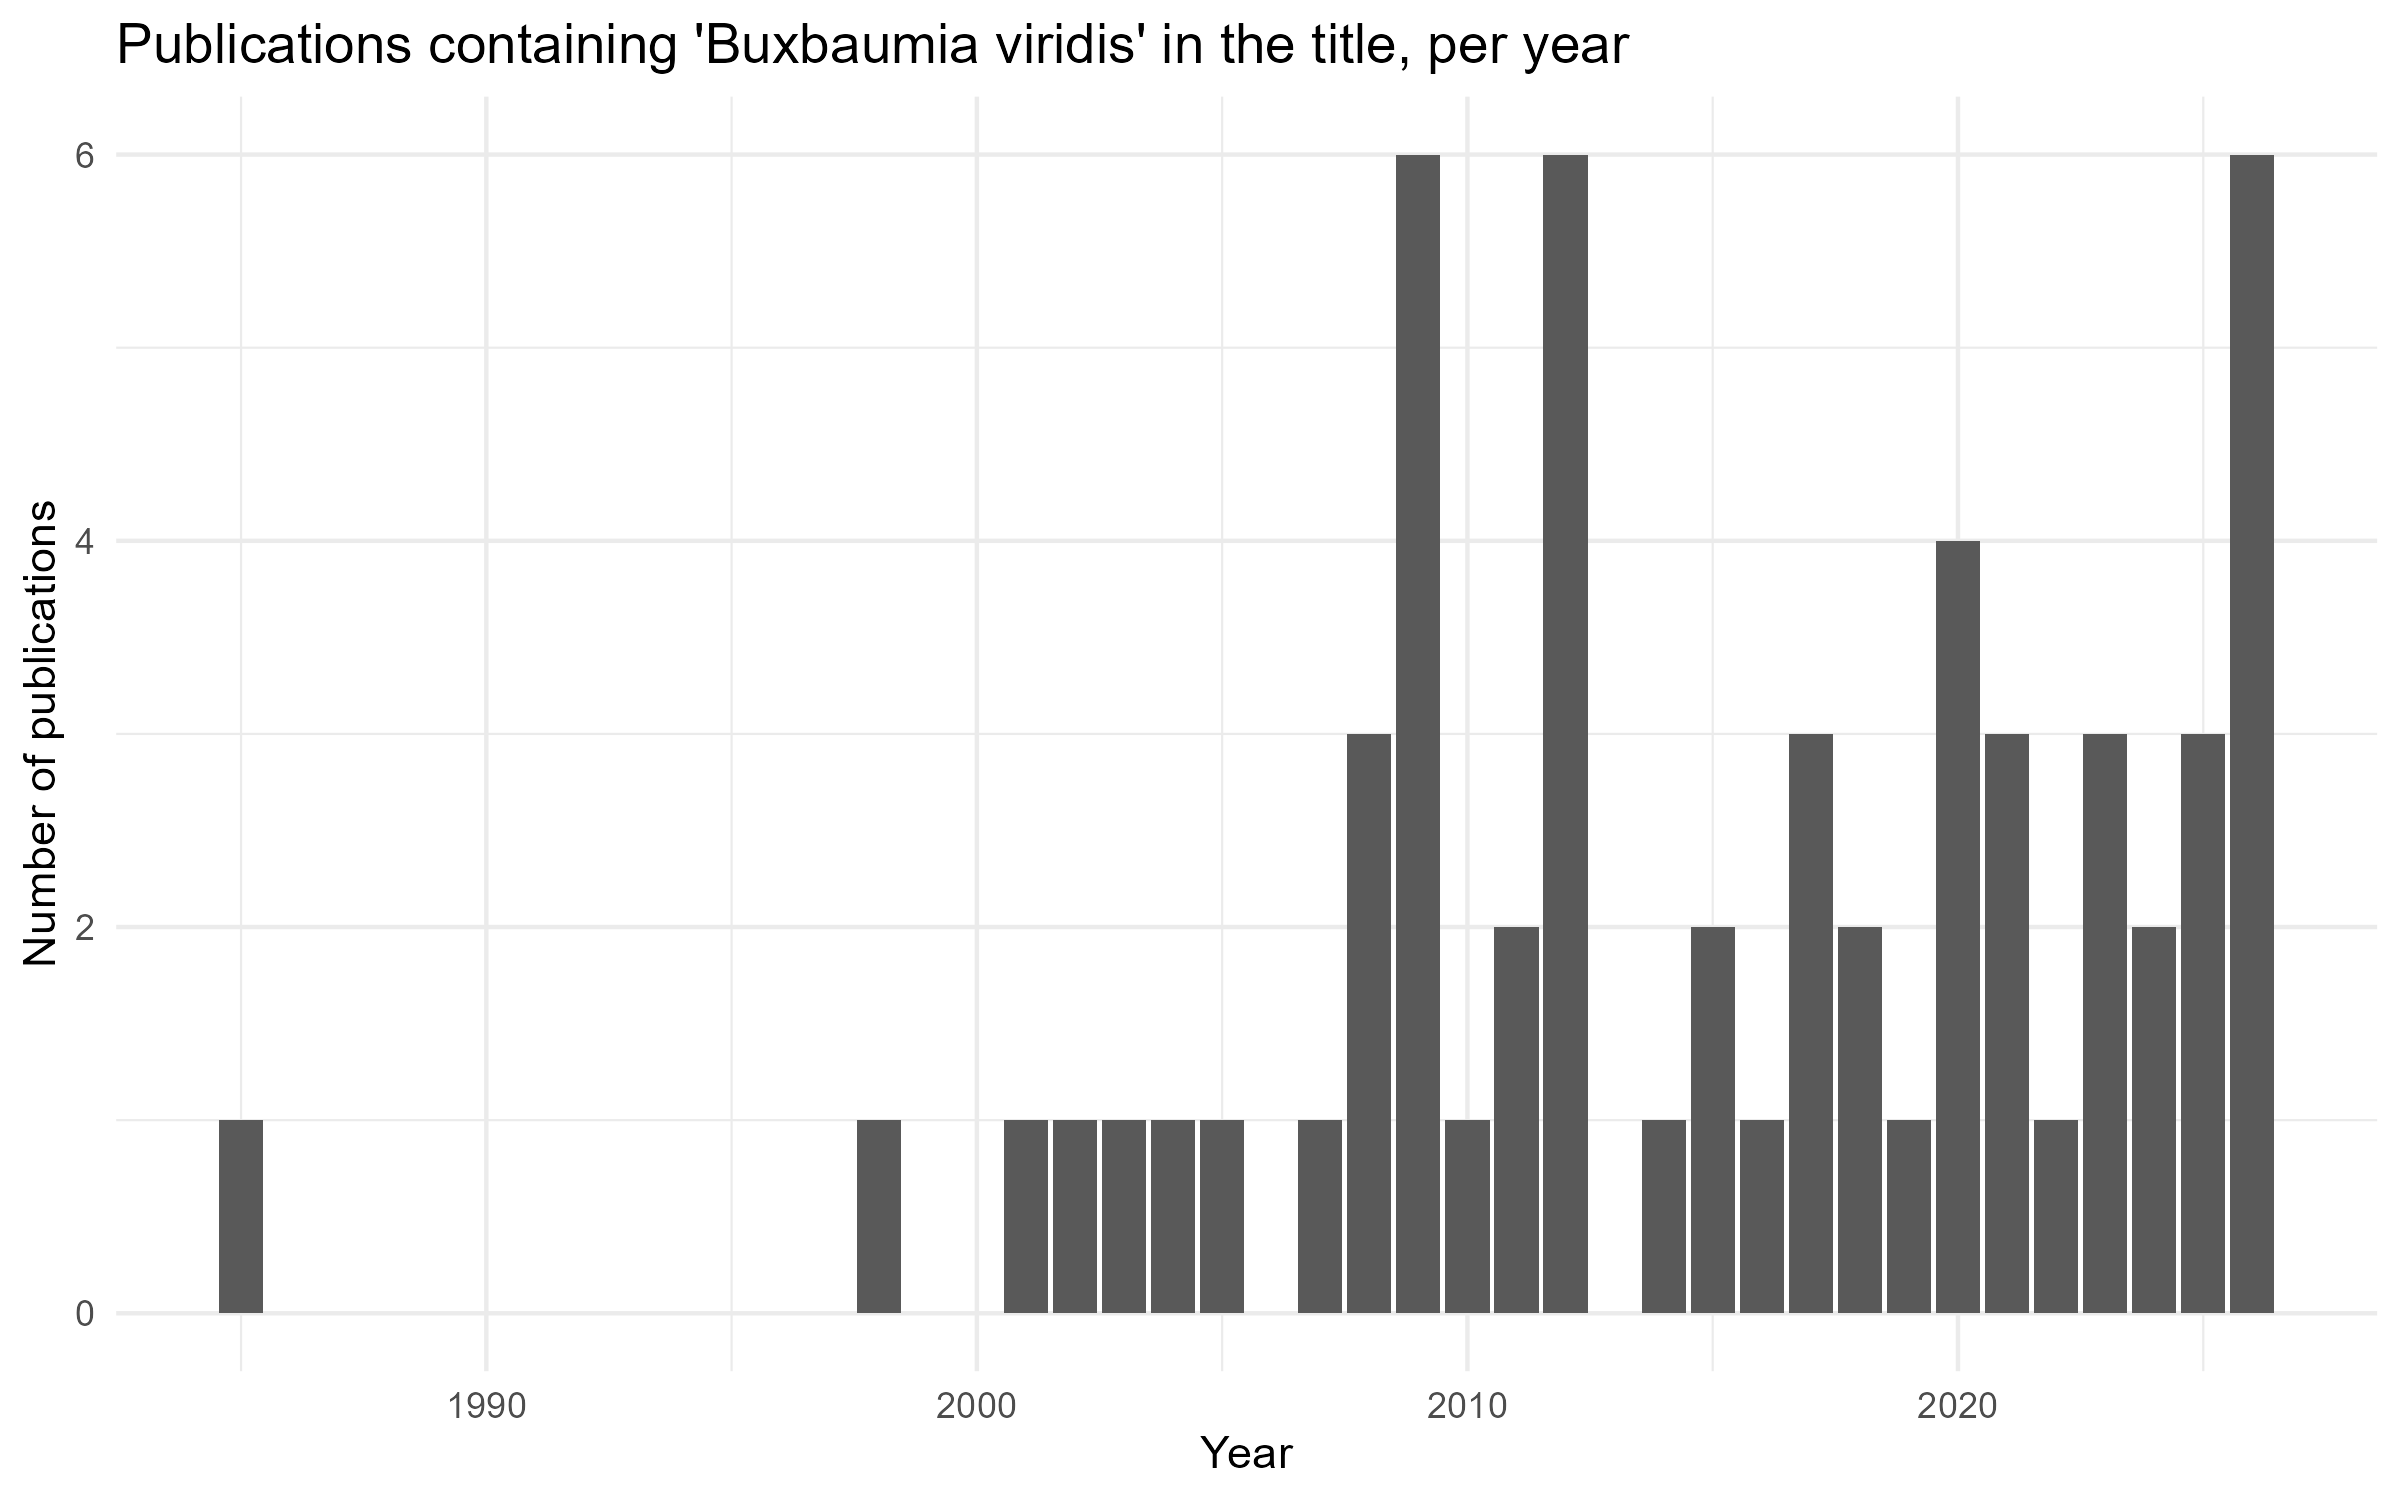
\includegraphics[keepaspectratio]{../02_Displays/Figures/B_viridis_publications.png}}
\end{center}

\subsection{\texorpdfstring{Ecology and distribution of \emph{Buxbaumia
viridis}}{Ecology and distribution of Buxbaumia viridis}}\label{ecology-and-distribution-of-buxbaumia-viridis}

\paragraph{Chorological distribution and geographic
scope}\label{chorological-distribution-and-geographic-scope}

\emph{Buxbaumia viridis} has a circumpolar distribution in the Northern
hemisphere, extending from Asia to North America and Europe (Offerhaus
et al., 2019). In Europe, its range is fragmented, extending from
southern Scandinavia to the southern mountain ranges (Infante and Heras,
2018). Recent papers indicate that its distribution ranges and
abundances have been underestimated, likely due to the underdetection of
the gametophyte (Brewczyński et al., 2021).

In France, the species is found in all major mountain ranges. The
discovery of populations consisting solely of gametophytes has
significantly expanded its known range to lowland region, sometimes at
elevations as low as 10 meters (Huggonot et al., 2023).

\paragraph{Ecology at the macrohabitat
scale}\label{ecology-at-the-macrohabitat-scale}

The species is sciaphilous and hygrophilous, restricted to coniferous
forests (spruce and fir-beech forests) in the montane and subalpine
zones. The optimal altitudinal range in France is between 900 and 1,600
m, although it can reach 2,000 m in the Alps (Offerhaus et al., 2019).
Canopy structure is a determining factor : the species prefers dense
forest cover (canopy closure between \textasciitilde70 and 85\%)
(Spitale and Mair, 2017). The probability of occurrence increases
significantly with basal area : a minimum threshold of \textasciitilde30
m²/ha, which is favorable for maintaining sufficient humidity and shade
(Vottier and Vallée, 2017). However, moderate canopy openness is thought
to promote sporophyte development, likely due to morning dew deposits
(Guillet et al., 2021). On a larger spatial scale, atmospheric humidity,
which depends on elevation, northness, and proximity to watercourses, is
a key factor for the species (Brewczyński et al., 2021).

\paragraph{Microhabitat-scale ecology and substrate
preferences}\label{microhabitat-scale-ecology-and-substrate-preferences}

\emph{B.viridis} is a saprolignicolous moss that colonizes coarse wood
debris (CWD) on the ground, and occasionally stumps. Conifers are the
predominant hosts, but certain deciduous species (beech, willow) are
colonized less frequently (Brewczyński et al., 2021). The species is a
pioneer on debarked wood but requires an advanced stage of decomposition
: the wood must be soft enough to absorb water (Guillet et al., 2021 ;
Offerhaus et al., 2019). The size of the CWD is not always a limiting
factor. Sporophytic populations are often associated with large CWD,
while the protonemal stage frequently occupies short pieces of wood with
small diameters. A site may have a high probability of \emph{B.viridis}
occurrence starting from a minimum threshold of CWD volume (necromass)
of \textasciitilde50 m³/ha (Spitale and Mair, 2017).

\paragraph{Spatial specificity of the life
cycle}\label{spatial-specificity-of-the-life-cycle}

The study of \emph{B.viridis} is complicated by the separation of its
two life stages. The sporophyte stage has been studied much more
extensively because it is much easier to observe to the naked eye. The
sporophyte is visible only when climatic conditions allow for fruiting
(cold, wet autumn). Being restricted to old-growth, high-altitude
forests, it has a smaller spatial distribution than the gametophyte
(Guillet et al., 2021). The gametophytic stage has a broader ecological
range and can persist in habitats considered suboptimal (plains,
deciduous forests, drier areas) without ever producing sporophytes. The
presence of gemmae allows for prolonged local survival even after
periods of drought (Hugonnot et al., 2023 ; Deme and Csiky, 2021).

\paragraph{Spatial dynamics and
dispersal}\label{spatial-dynamics-and-dispersal}

This species appears to be limited more by its dispersal capabilities
than by habitat availability. Although wind accounts for some spore
transport, long-distance dispersal and dispersal within closed forest
canopies likely depend on biotic vectors. Small mammals and birds may
act as potential vectors, although rodents are also predators that
consume the capsules before they mature (Kropik et al., 2020). Herbivory
by slugs (Arion sp.) may also constitute a significant mortality factor
(Infante and Heras, 2018).

\paragraph{Impacts of forest
management}\label{impacts-of-forest-management}

Silvicultural management directly influences the species' spatial
distribution by altering the microclimate and the stock of CWD. Logging
is not necessarily a threat if it maintains a sufficient volume of CWD
and avoids clear-cutting, which dries out the habitat (Offerhaus et al.,
2019). For example, Vottier and Vallée (2017) showed that proximity to
forest roads does not negatively impact the presence or abundance of
sporophytes, provided that suitable substrates are not destroyed during
logging operations. Most studies conclude that effective conservation of
\emph{B.viridis} requires spatial and temporal continuity of decomposing
substrates within forest stands (Kropik et al., 2020 ; Puntillo and
Puntillo, 2024).

\subsection{Local distribution of obligatory
species}\label{local-distribution-of-obligatory-species}

\begin{tcolorbox}[enhanced jigsaw, breakable, colback=white, opacityback=0, bottomtitle=1mm, arc=.35mm, rightrule=.15mm, colbacktitle=quarto-callout-note-color!10!white, titlerule=0mm, colframe=quarto-callout-note-color-frame, toprule=.15mm, opacitybacktitle=0.6, coltitle=black, left=2mm, bottomrule=.15mm, leftrule=.75mm, toptitle=1mm, title=\textcolor{quarto-callout-note-color}{\faInfo}\hspace{0.5em}{Title idea}]

\emph{To be completed with a literature review}

\end{tcolorbox}

\subsection{Bibliographic hole and objectives of the
study}\label{bibliographic-hole-and-objectives-of-the-study}

Most studies have focused on chorology or niche models. This literature
suggests that \emph{B.viridis} simply follows the resource as long as
climatic conditions are favorable and there is a sufficient amount of
CWD. However, Kropik et al.~(2020) note that suitable habitats remain
unoccupied, suggesting that dispersal is a limiting factor. To date, no
research has been conducted on the fine-scale spatial structure of this
moss within a single forest plot. The objective of this work is to
conduct such research in order to distinguish between the resource
pattern and the colonization pattern (\emph{Buxbaumia} specific spatial
processes). This study aims to distinguish between potential niche and
realized niche, in order to understand how the species colonizes the
available space. To do this, we have access to spatialized data that
enables point pattern analysis.

\begin{tcolorbox}[enhanced jigsaw, breakable, colback=white, opacityback=0, bottomtitle=1mm, arc=.35mm, rightrule=.15mm, colbacktitle=quarto-callout-note-color!10!white, titlerule=0mm, colframe=quarto-callout-note-color-frame, toprule=.15mm, opacitybacktitle=0.6, coltitle=black, left=2mm, bottomrule=.15mm, leftrule=.75mm, toptitle=1mm, title=\textcolor{quarto-callout-note-color}{\faInfo}\hspace{0.5em}{Title idea}]

\textbf{\emph{Role of dispersal and microhabitat on the spatial
distribution of a coarse wood-associated moss at the local scale.}}

\end{tcolorbox}

\subsection{Concept map}\label{concept-map}

\begin{tcolorbox}[enhanced jigsaw, breakable, colback=white, opacityback=0, bottomtitle=1mm, arc=.35mm, rightrule=.15mm, colbacktitle=quarto-callout-note-color!10!white, titlerule=0mm, colframe=quarto-callout-note-color-frame, toprule=.15mm, opacitybacktitle=0.6, coltitle=black, left=2mm, bottomrule=.15mm, leftrule=.75mm, toptitle=1mm, title=\textcolor{quarto-callout-note-color}{\faInfo}\hspace{0.5em}{NB}]

\emph{To be updated}

\end{tcolorbox}

\begin{center}
\pandocbounded{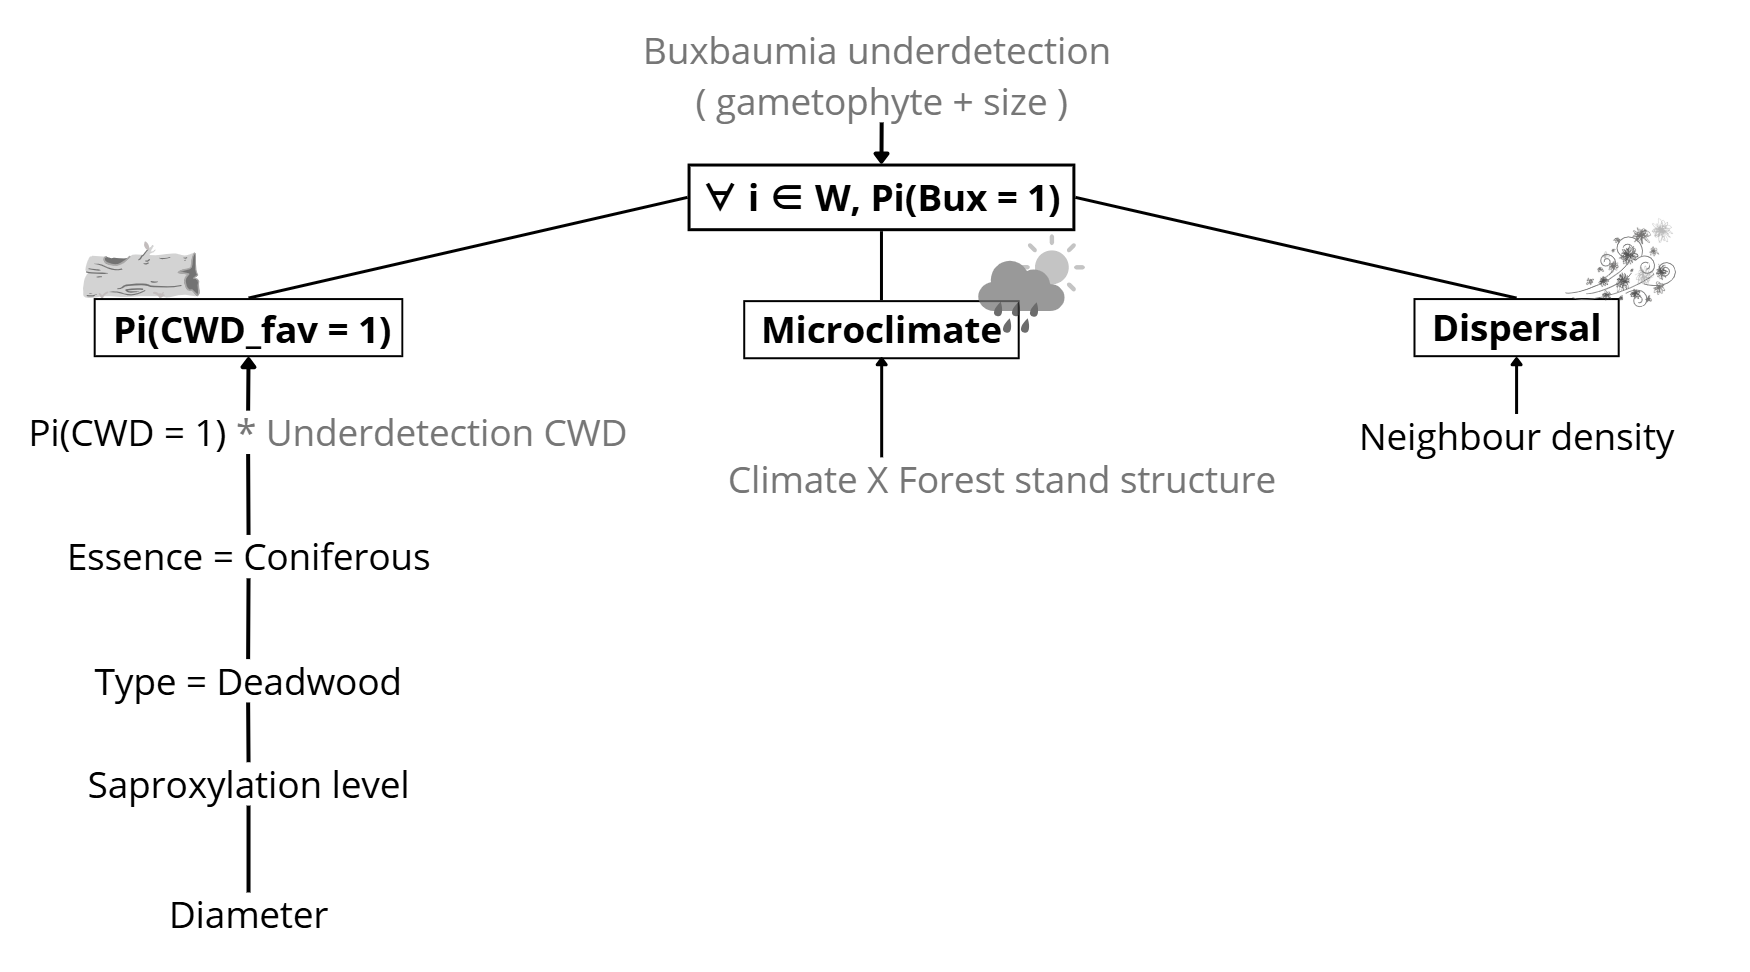
\includegraphics[keepaspectratio]{../02_Displays/Figures/concept_map.png}}
\end{center}

\section{Data collection}\label{data-collection}

\begin{tcolorbox}[enhanced jigsaw, breakable, colback=white, opacityback=0, bottomtitle=1mm, arc=.35mm, rightrule=.15mm, colbacktitle=quarto-callout-note-color!10!white, titlerule=0mm, colframe=quarto-callout-note-color-frame, toprule=.15mm, opacitybacktitle=0.6, coltitle=black, left=2mm, bottomrule=.15mm, leftrule=.75mm, toptitle=1mm, title=\textcolor{quarto-callout-note-color}{\faInfo}\hspace{0.5em}{NB}]

\emph{To be Completed}

\end{tcolorbox}

\section{Data Structure \& Management}\label{data-structure-management}

\begin{tcolorbox}[enhanced jigsaw, breakable, colback=white, opacityback=0, bottomtitle=1mm, arc=.35mm, rightrule=.15mm, colbacktitle=quarto-callout-note-color!10!white, titlerule=0mm, colframe=quarto-callout-note-color-frame, toprule=.15mm, opacitybacktitle=0.6, coltitle=black, left=2mm, bottomrule=.15mm, leftrule=.75mm, toptitle=1mm, title=\textcolor{quarto-callout-note-color}{\faInfo}\hspace{0.5em}{NB}]

\emph{To be Completed}

\end{tcolorbox}

\section{Analysis}\label{analysis}

\subsection{Exploratory analysis}\label{exploratory-analysis}

The spatial structure of deadwood substrates and their colonisation by
\emph{Buxbaumia viridis} was investigated using two second-order
statistics. The Pair Correlation Function (PCF) quantifies the relative
density of point pairs separated by a distance r, compared to a complete
spatial randomness (CSR) distribution ; values of g(r) \textgreater{} 1
indicate spatial aggregation at scale r, and g(r) = 1 is randomness. The
Mark Connection Function (MCF) estimates the probability that two points
at distance r both show a given mark (here, colonisation by
\emph{B.viridis} --\textgreater pres-pres) under a random labelling null
hypothesis. Departures above the simulation envelope therefore indicate
that colonised substrates are spatially clustered independently of the
underlying CWD distribution.

\textbf{Results :} PCF profiles were strikingly consistent across all
four study sites : g(r) reached very high values at short distances (r
\textless{} 2--3 m), well above the simulation envelope, before rapidly
converging to unity beyond r ≈ 5--10 m, indicating strong but spatially
confined aggregation of deadwood at the metric scale, likely driven by
the localised occurrence of decaying trees or branch falls.

MCF results, however, varied markedly among sites and tracked closely
with overall colonisation rates. At sites with low occupancy (M2, 7\%;
M5, 6\%), the pres-pres MCF curve remained within the simulation
envelope across all distances, providing no evidence of non-random
spatial clustering of colonised substrates beyond that expected by
chance. At M4 (8\%), a moderate positive departure was detected at
intermediate distances (r ≈ 5--15 m), suggesting a perceptible tendency
toward aggregation. By contrast, at M3 (the most heavily colonised site
(22\%)), the MCF curve exceeded the envelope at short distances and
remained elevated throughout, revealing a strong and statistically
significant aggregation of colonised substrates. Taken together, these
results indicate that the spatial clustering of \emph{B.viridis}
occurrences is not merely a by-product of deadwood distribution, but
reflects an independent aggregative process. This signal is consistent
with short-distance spore dispersal, local source effects, or fine-scale
environmental filtering, but seems to be rare or hard to detect (have to
be carefull here, n=4).

\subsection{PPM}\label{ppm}

Colonisation intensity was modelled across the four study sites using
inhomogeneous Poisson point process models (PPM) fitted by maximum
likelihood, with log-linear effects of three spatially continuous
covariates: local deadwood density weighted by diameter at a 10 m
bandwidth (dens10), smoothed local altitude (alt), and substrate
saproxylation stage (sap).

\[\log \lambda(u) = \beta_0 + \beta_1 \cdot \text{dens10}(u) + \beta_2 \cdot \text{alt}(u) + \beta_3 \cdot \text{sap}(u)\]

Covariates were derived from the full deadwood point pattern using
kernel smoothing : dens10 was computed as a diameter-weighted kernel
density estimate (σ = 10 m) ; alt was obtained by spatial smoothing of
raw elevation values (σ = 15 m) ; sap was smoothed from substrate-level
saproxylation scores (σ = 3 m). All covariates were standardised (zero
mean, unit variance) prior to model fitting to ensure comparability of
coefficients across sites.

\textbf{Results :} Substrate saproxylation was the dominant and most
consistent driver of colonisation intensity across all four sites, with
large positive coefficients ranging from β = 1.54 (M3) to β = 2.44 (M5),
all highly significant (p \textless{} 0.001), confirming that \emph{B.
viridis} colonisation is strongly concentrated on the most decomposed
substrates regardless of site. Local deadwood density showed a weaker
but consistently positive and significant effect at all sites (β =
0.31--0.48, p \textless{} 0.05), suggesting that substrate availability
at the neighbourhood scale contributes independently of substrate
quality. The effect of local altitude was more variable : positive and
significant at M2 (β = 0.72, p \textless{} 0.01) and M3 (β = 0.22, p
\textless{} 0.01), but non-significant at M4 and M5 (β = 0.05, p = 0.72
and β = −0.37, p = 0.11 respectively), indicating that fine-scale
topographic moisture gradients may modulate colonisation at some sites
but are not a general driver across the study area.

\textbf{Limits :} One important limitation concerns the inclusion of
local deadwood density (dens10) as a covariate. Because colonised
substrates are themselves deadwood, a positive effect of dens10 on
colonisation intensity is to some extent tautological : areas with more
deadwood will mechanically contain more colonised deadwood, regardless
of any biological preference. The dens10 effect should therefore be
interpreted with caution, as a descriptor of spatial co-occurrence
rather than evidence of a causal effect of substrate density on
colonisation probability.

Furthermore, PPMs are restricted to spatially continuous covariates.
Categorical substrate variables (tree species, substrate type) could not
be included directly and required spatial interpolation of inherently
discrete values, a method widely criticised for its imprecision.

\subsection{Joint INLA model}\label{joint-inla-model}

\subsubsection{Methods}\label{methods}

The Bayesian model directly addresses this confounding issue by
modelling colonisation as a Bernoulli outcome at the individual
substrate level that is : given that a deadwood piece is present, what
is the probability that it is colonised by \emph{B.viridis}?

This formulation conditions on substrate availability by design.
Furthermore, the Bayesian framework implemented in INLA offers a
treatment of uncertainty propagation : rather than producing point
estimates with asymptotic standard errors, INLA computes the full
posterior distribution of each parameter, naturally integrating
uncertainty across all levels of the model without relying on
large-sample approximations. This is valuable in the present context,
where sample sizes vary substantially across sites and colonisation
rates are low, making frequentist confidence intervals potentially
unreliable. The posterior distributions obtained for each covariate
effect thus reflect genuine inferential uncertainty given the data, and
credible intervals can be interpreted.

A preliminary simple INLA model was fitted at the individual substrate
level, confirming the importance of saproxylation stage and diameter as
drivers of colonisation. The joint model was then developed to
additionally account for the spatial structure of deadwood distribution.
To jointly model the spatial distribution of CWD and the colonisation
probability of \emph{Buxbaumia viridis}, we implemented a joint latent
Gaussian model fitted using INLA (Integrated Nested Laplace
Approximation ; Rue et al., 2009) combined with the SPDE approach
(Lindgren et al., 2011). The model couples two processes through a
shared spatial random field, allowing uncertainty from the first process
to propagate into the second without double-fitting.

\textbf{Process 1 --- Log-Gaussian Cox Process (LGCP) for deadwood
distribution.} The spatial distribution of all deadwood substrates was
modelled as an inhomogeneous Poisson process on the continuous domain,
with log-intensity :

\[\log \lambda_1(s) = \mu_1 + w_1(s)\]

where \(\mu_1\) is a global intercept and \(w_1(s)\) is a zero-mean
Matérn Gaussian random field (SPDE approximation, \(\alpha = 2\))
capturing the latent spatial structure of CWD clustering. Integration
weights were computed from the Voronoi dual mesh areas, capped at five
times their median to ensure numerical stability of peripheral nodes
(Simpson et al., 2016 ; Krainski et al., 2018). The field \(w_1\) was
replicated independently across the four study sites, with shared
hyperparameters (range \(\rho_1\), marginal standard deviation
\(\sigma_1\)).

\textbf{Process 2 --- Binomial model for \emph{B.viridis} colonisation.}
Colonisation probability at each substrate \(i\) was modelled as:

\[
\begin{aligned}
\text{logit}(p_i) = \, & \alpha + \beta_{\text{diam}} \cdot \text{diam}_i 
+ \sum_{k=2}^{5} \beta_{S_k} \cdot \mathbf{1}[S\_MAX_i = k] \\
& + \beta_{\text{ess}} \cdot \mathbf{1}[\text{conifer}] 
+ \beta_{\text{sup}} \cdot \mathbf{1}[\text{stump}] 
+ \beta_s \cdot w_1(s_i) + w_2(s_i)
\end{aligned}
\]

where \(\alpha\) is an intercept; \(\text{diam}_i\) is the standardised
substrate diameter; \(S\_MAX\) is the saproxylation stage (reference =
stage 1); \(\beta_{\text{ess}}\) and \(\beta_{\text{sup}}\) are
contrasts for conifer substrates (reference = deciduous) and stumps
(reference = logs), respectively. The term \(\beta_s \cdot w_1(s_i)\) is
the coupling term : the shared field \(w_1\), estimated in Process 1,
enters Process 2 multiplied by a freely estimated coefficient
\(\beta_s\), implemented via the copy functionality of R-INLA. If
\(\beta_s > 0\), areas of high deadwood density positively influence
colonisation probability, while \(\beta_s \approx 0\) indicates that
colonisation is independent of deadwood spatial structure once
individual substrate covariates are controlled. This coupling propagates
uncertainty from Process 1 into Process 2. Finally, \(w_2(s_i)\) is an
independent residual spatial field capturing remaining autocorrelation
in \emph{B.viridis} occurrence after accounting for all covariates and
the shared field.

\textbf{Spatial fields and priors :} Both fields \(w_1\) and \(w_2\)
were approximated using the SPDE approach on a common triangulated mesh
(max edge = 5 m inner / 20 m outer, cutoff = 1 m), and replicated across
sites. Penalized Complexity (PC) priors were placed on their range and
marginal standard deviation. For \(w_1\), the range prior was set to
\(P(\rho_1 < 20\text{ m}) = 0.9\), reflecting the expectation that
deadwood clustering operates at the local scale of tree falls (a few
metres), and preventing competition with \(w_2\) which could otherwise
converge to the same spatial scale and render the joint model
non-identifiable. For \(w_2\), a weakly informative prior was used
(\(P(\rho_2 < 50\text{ m}) = 0.5\)), allowing the data to freely
estimate the residual autocorrelation range. The robustness of
fixed-effect estimates to prior specification was assessed through a
sensitivity analysis across multiple prior configurations, which
confirmed the stability of Process 2 coefficients.

\textbf{INLA joint model function code}

\begin{Shaded}
\begin{Highlighting}[]
\CommentTok{\# =============================================================================}
\CommentTok{\# fun\_joint\_inla.R}
\CommentTok{\# Joint INLA model : LGCP (deadwood pattern) + Binomial (Buxbaumia viridis)}
\CommentTok{\# Uncertainty propagation via shared spatial field w1}
\CommentTok{\#}
\CommentTok{\# Model architecture :}
\CommentTok{\#}
\CommentTok{\#   Process 1 — Poisson LGCP on all deadwood substrates (DW)}
\CommentTok{\#     Predictor  : η1\_k(s) = μ1 + w1\_k(s)}
\CommentTok{\#     Likelihood : y\_node \textasciitilde{} Poisson(a\_node * exp(η1\_k(s)))}
\CommentTok{\#     where a\_node = Voronoi area of the node (dual mesh integration weight),}
\CommentTok{\#     truncated at 5× the median to avoid numerical instability at peripheral}
\CommentTok{\#     nodes (Simpson et al. 2016, Krainski et al. 2018)}
\CommentTok{\#     and w1\_k \textasciitilde{} SPDE Matern(range1, σ1), replicated per site k, sum{-}to{-}zero}
\CommentTok{\#}
\CommentTok{\#   Process 2 — Binomial on Buxbaumia viridis presence}
\CommentTok{\#     logit(p\_i) = intercept\_p2}
\CommentTok{\#                + β\_diam  * Diameter\_sc}
\CommentTok{\#                + β\_smax2 * S\_MAX2 + β\_smax3 * S\_MAX3  (ref = S\_MAX1)}
\CommentTok{\#                + β\_smax4 * S\_MAX4 + β\_smax5 * S\_MAX5}
\CommentTok{\#                + β\_ess   * Essence\_Conifer             (ref = Broadleaf)}
\CommentTok{\#                + β\_sup   * Type\_Stump                  (ref = DWS)}
\CommentTok{\#                + β\_s     * w1\_k(s\_i)   [free coupling coefficient, estimated]}
\CommentTok{\#                + w2\_k(s\_i)              [process{-}specific residual field]}
\CommentTok{\#     where w2\_k \textasciitilde{} SPDE Matern(range2, σ2), replicated per site k}
\CommentTok{\#}
\CommentTok{\# Coupling between processes :}
\CommentTok{\#   Field w1 enters simultaneously into the LGCP (process 1) and the binomial}
\CommentTok{\#   predictor (process 2) via a freely estimated coupling coefficient β\_s}
\CommentTok{\#   (R{-}INLA "copy" feature). If β\_s \textgreater{} 0, areas of high DW density favour}
\CommentTok{\#   Buxbaumia presence, propagating uncertainty from process 1 into process 2}
\CommentTok{\#   without double{-}fitting.}
\CommentTok{\#   In this dataset, β\_s ≈ 0 across all tested configurations : local DW}
\CommentTok{\#   density has no detectable effect on Buxbaumia presence once individual}
\CommentTok{\#   covariates and residual autocorrelation are controlled for}
\CommentTok{\#   (see prior sensitivity analysis).}
\CommentTok{\#}
\CommentTok{\# Fixed effects handling :}
\CommentTok{\#   Categorical covariates (S\_MAX, Essence, Type) are manually encoded as 0/1}
\CommentTok{\#   indicators to ensure correct identification of the reference level in the}
\CommentTok{\#   presence of the explicit intercept intercept\_p2 and the suppression of the}
\CommentTok{\#   global intercept ({-}1 in the INLA formula).}
\CommentTok{\#   Essence "Indeterminate" is excluded from the data (3.7\% of observations).}
\CommentTok{\#}
\CommentTok{\# Model identifiability :}
\CommentTok{\#   Without constraints on w1, both fields spontaneously converge towards the}
\CommentTok{\#   same spatial scale (\textasciitilde{}80 m), creating competition that renders the model}
\CommentTok{\#   non{-}identifiable. The PC prior on the range of w1 (P(range \textless{} 20 m) = 0.9)}
\CommentTok{\#   cleanly separates the two processes : w1 operates at \textasciitilde{}5 m (local DW}
\CommentTok{\#   clustering) and w2 at \textasciitilde{}82 m (residual Buxbaumia autocorrelation). The}
\CommentTok{\#   robustness of fixed effects to this constraint was verified by sensitivity}
\CommentTok{\#   analysis across multiple prior configurations.}
\CommentTok{\#}
\CommentTok{\# Multi{-}site structure :}
\CommentTok{\#   Fields w1 and w2 are replicated across the 4 sites (M2, M3, M4, M5)}
\CommentTok{\#   via replicate = site\_id. Hyperparameters (range, σ) are shared across}
\CommentTok{\#   sites but field realisations are independent per site.}
\CommentTok{\#   Coordinates are centred by site before mesh construction.}
\CommentTok{\#   Releveling of Site (ref = "M2") ensures consistent replicate ordering}
\CommentTok{\#   between w1 and w2 regardless of raw data ordering.}
\CommentTok{\#}
\CommentTok{\# References :}
\CommentTok{\#   Rue, Martino \& Chopin (2009)}
\CommentTok{\#   Illian et al. (2013) Methods in Ecology and Evolution 4:305{-}315}
\CommentTok{\#   Lindgren, Rue \& Lindstrom (2011) JRSS{-}B 73:423{-}498}
\CommentTok{\#     {-}{-}\textgreater{} SPDE : Matern Gaussian field approximation}
\CommentTok{\#   Krainski et al. (2018) Advanced Spatial Modeling with SPDE}
\CommentTok{\#   Simpson et al. (2016) Statistical Science 32:1{-}29}
\CommentTok{\# =============================================================================}

\NormalTok{fun\_joint\_inla }\OtherTok{\textless{}{-}} \ControlFlowTok{function}\NormalTok{(}
\NormalTok{  data,}
  \CommentTok{\# Mesh parameters}
  \AttributeTok{max.edge =} \FunctionTok{c}\NormalTok{(}\DecValTok{5}\NormalTok{, }\DecValTok{20}\NormalTok{),}
  \AttributeTok{cutoff =} \DecValTok{1}\NormalTok{,}
  \AttributeTok{offset =} \FunctionTok{c}\NormalTok{(}\DecValTok{10}\NormalTok{, }\DecValTok{30}\NormalTok{),}
  \CommentTok{\# PC priors for w1 (deadwood spatial field)}
  \AttributeTok{prior.range1 =} \FunctionTok{c}\NormalTok{(}\DecValTok{20}\NormalTok{, }\FloatTok{0.9}\NormalTok{),}
  \AttributeTok{prior.sigma1 =} \FunctionTok{c}\NormalTok{(}\DecValTok{1}\NormalTok{, }\FloatTok{0.5}\NormalTok{),}
  \CommentTok{\# PC priors for w2 (residual Buxbaumia field)}
  \AttributeTok{prior.range2 =} \FunctionTok{c}\NormalTok{(}\DecValTok{50}\NormalTok{, }\FloatTok{0.5}\NormalTok{),}
  \AttributeTok{prior.sigma2 =} \FunctionTok{c}\NormalTok{(}\DecValTok{1}\NormalTok{, }\FloatTok{0.01}\NormalTok{)}
\NormalTok{) \{}
  \CommentTok{\# {-}{-}{-}{-}{-}{-}{-}{-}{-}{-}{-}{-}{-}{-}{-}{-}{-}{-}{-}{-}{-}{-}{-}{-}{-}{-}{-}{-}{-}{-}{-}{-}{-}{-}{-}{-}{-}{-}{-}{-}{-}{-}{-}{-}{-}{-}{-}{-}{-}{-}{-}{-}{-}{-}{-}{-}{-}{-}{-}{-}{-}{-}{-}{-}{-}{-}{-}{-}{-}{-}{-}{-}{-}{-}{-}}
  \CommentTok{\# 1. Data preparation}
  \CommentTok{\# {-}{-}{-}{-}{-}{-}{-}{-}{-}{-}{-}{-}{-}{-}{-}{-}{-}{-}{-}{-}{-}{-}{-}{-}{-}{-}{-}{-}{-}{-}{-}{-}{-}{-}{-}{-}{-}{-}{-}{-}{-}{-}{-}{-}{-}{-}{-}{-}{-}{-}{-}{-}{-}{-}{-}{-}{-}{-}{-}{-}{-}{-}{-}{-}{-}{-}{-}{-}{-}{-}{-}{-}{-}{-}{-}}
\NormalTok{  n\_obs\_start }\OtherTok{\textless{}{-}} \FunctionTok{nrow}\NormalTok{(data)}

\NormalTok{  df }\OtherTok{\textless{}{-}}\NormalTok{ data }\SpecialCharTok{\%\textgreater{}\%}
    \FunctionTok{filter}\NormalTok{(Essence }\SpecialCharTok{!=} \StringTok{"Indéterminé"}\NormalTok{) }\SpecialCharTok{\%\textgreater{}\%}
    \FunctionTok{mutate}\NormalTok{(}
      \AttributeTok{P\_Bux =} \FunctionTok{as.integer}\NormalTok{(P\_Bux),}
      \AttributeTok{Site =} \FunctionTok{as.factor}\NormalTok{(Site),}
      \AttributeTok{Diam\_sc =} \FunctionTok{as.numeric}\NormalTok{(}\FunctionTok{scale}\NormalTok{(Diameter)),}
      \AttributeTok{Sap\_max =} \FunctionTok{as.factor}\NormalTok{(Sap\_max),}
      \AttributeTok{Essence =} \FunctionTok{as.factor}\NormalTok{(Essence),}
      \AttributeTok{Type =} \FunctionTok{as.factor}\NormalTok{(Type)}
\NormalTok{    )}

  \FunctionTok{message}\NormalTok{(}\FunctionTok{paste0}\NormalTok{(}
    \StringTok{"N observations used : "}\NormalTok{, }\FunctionTok{nrow}\NormalTok{(df),}
    \StringTok{" ("}\NormalTok{, n\_obs\_start }\SpecialCharTok{{-}} \FunctionTok{nrow}\NormalTok{(df), }\StringTok{" removed, "}\NormalTok{,}
    \FunctionTok{round}\NormalTok{(}\DecValTok{100} \SpecialCharTok{{-}}\NormalTok{ (}\FunctionTok{nrow}\NormalTok{(df) }\SpecialCharTok{/}\NormalTok{ n\_obs\_start }\SpecialCharTok{*} \DecValTok{100}\NormalTok{), }\DecValTok{2}\NormalTok{), }\StringTok{"\%)"}
\NormalTok{  ))}

  \CommentTok{\# Relevel : ensures consistent replicate ordering across w1 and w2}
\NormalTok{  df}\SpecialCharTok{$}\NormalTok{Site }\OtherTok{\textless{}{-}} \FunctionTok{relevel}\NormalTok{(df}\SpecialCharTok{$}\NormalTok{Site, }\AttributeTok{ref =} \StringTok{"M2"}\NormalTok{)}
\NormalTok{  df}\SpecialCharTok{$}\NormalTok{Sap\_max }\OtherTok{\textless{}{-}} \FunctionTok{relevel}\NormalTok{(df}\SpecialCharTok{$}\NormalTok{Sap\_max, }\AttributeTok{ref =} \StringTok{"1"}\NormalTok{)}

  \CommentTok{\# {-}{-}{-}{-}{-}{-}{-}{-}{-}{-}{-}{-}{-}{-}{-}{-}{-}{-}{-}{-}{-}{-}{-}{-}{-}{-}{-}{-}{-}{-}{-}{-}{-}{-}{-}{-}{-}{-}{-}{-}{-}{-}{-}{-}{-}{-}{-}{-}{-}{-}{-}{-}{-}{-}{-}{-}{-}{-}{-}{-}{-}{-}{-}{-}{-}{-}{-}{-}{-}{-}{-}{-}{-}{-}{-}}
  \CommentTok{\# 2. Local coordinates and site indexing}
  \CommentTok{\# {-}{-}{-}{-}{-}{-}{-}{-}{-}{-}{-}{-}{-}{-}{-}{-}{-}{-}{-}{-}{-}{-}{-}{-}{-}{-}{-}{-}{-}{-}{-}{-}{-}{-}{-}{-}{-}{-}{-}{-}{-}{-}{-}{-}{-}{-}{-}{-}{-}{-}{-}{-}{-}{-}{-}{-}{-}{-}{-}{-}{-}{-}{-}{-}{-}{-}{-}{-}{-}{-}{-}{-}{-}{-}{-}}
\NormalTok{  df }\OtherTok{\textless{}{-}}\NormalTok{ df }\SpecialCharTok{\%\textgreater{}\%}
    \FunctionTok{group\_by}\NormalTok{(Site) }\SpecialCharTok{\%\textgreater{}\%}
    \FunctionTok{mutate}\NormalTok{(}
      \AttributeTok{X\_loc =}\NormalTok{ X }\SpecialCharTok{{-}} \FunctionTok{mean}\NormalTok{(X),}
      \AttributeTok{Y\_loc =}\NormalTok{ Y }\SpecialCharTok{{-}} \FunctionTok{mean}\NormalTok{(Y)}
\NormalTok{    ) }\SpecialCharTok{\%\textgreater{}\%}
    \FunctionTok{ungroup}\NormalTok{()}

\NormalTok{  df}\SpecialCharTok{$}\NormalTok{site\_id }\OtherTok{\textless{}{-}} \FunctionTok{as.integer}\NormalTok{(df}\SpecialCharTok{$}\NormalTok{Site)}
\NormalTok{  n\_sites }\OtherTok{\textless{}{-}} \FunctionTok{nlevels}\NormalTok{(df}\SpecialCharTok{$}\NormalTok{Site)}
\NormalTok{  coords\_loc }\OtherTok{\textless{}{-}} \FunctionTok{as.matrix}\NormalTok{(df[, }\FunctionTok{c}\NormalTok{(}\StringTok{"X\_loc"}\NormalTok{, }\StringTok{"Y\_loc"}\NormalTok{)])}
\NormalTok{  df}\SpecialCharTok{$}\NormalTok{row\_id }\OtherTok{\textless{}{-}} \FunctionTok{seq\_len}\NormalTok{(}\FunctionTok{nrow}\NormalTok{(df))}

  \CommentTok{\# {-}{-}{-}{-}{-}{-}{-}{-}{-}{-}{-}{-}{-}{-}{-}{-}{-}{-}{-}{-}{-}{-}{-}{-}{-}{-}{-}{-}{-}{-}{-}{-}{-}{-}{-}{-}{-}{-}{-}{-}{-}{-}{-}{-}{-}{-}{-}{-}{-}{-}{-}{-}{-}{-}{-}{-}{-}{-}{-}{-}{-}{-}{-}{-}{-}{-}{-}{-}{-}{-}{-}{-}{-}{-}{-}}
  \CommentTok{\# 3. Shared mesh}
  \CommentTok{\# {-}{-}{-}{-}{-}{-}{-}{-}{-}{-}{-}{-}{-}{-}{-}{-}{-}{-}{-}{-}{-}{-}{-}{-}{-}{-}{-}{-}{-}{-}{-}{-}{-}{-}{-}{-}{-}{-}{-}{-}{-}{-}{-}{-}{-}{-}{-}{-}{-}{-}{-}{-}{-}{-}{-}{-}{-}{-}{-}{-}{-}{-}{-}{-}{-}{-}{-}{-}{-}{-}{-}{-}{-}{-}{-}}
  \CommentTok{\# INLA estimates the latent spatial fields at triangle vertices, then}
  \CommentTok{\# interpolates to observation locations via the projection matrix A.}
  \CommentTok{\# Small triangles near data (max.edge[1]), larger ones further away}
  \CommentTok{\# (max.edge[2]) to reduce computation cost without losing local resolution.}
\NormalTok{  mesh }\OtherTok{\textless{}{-}} \FunctionTok{fm\_mesh\_2d\_inla}\NormalTok{(}
    \AttributeTok{loc =}\NormalTok{ coords\_loc,}
    \AttributeTok{max.edge =}\NormalTok{ max.edge,}
    \AttributeTok{cutoff =}\NormalTok{ cutoff, }\CommentTok{\# observations closer than cutoff metres are merged}
    \CommentTok{\# in the mesh to avoid overly small triangles}
    \AttributeTok{offset =}\NormalTok{ offset }\CommentTok{\# mesh extension beyond observed area to avoid}
    \CommentTok{\# spatial field boundary effects}
\NormalTok{  )}
\NormalTok{  n\_nodes }\OtherTok{\textless{}{-}}\NormalTok{ mesh}\SpecialCharTok{$}\NormalTok{n}
  \FunctionTok{message}\NormalTok{(}\FunctionTok{paste0}\NormalTok{(}\StringTok{"Mesh : "}\NormalTok{, n\_nodes, }\StringTok{" nodes"}\NormalTok{))}

\NormalTok{  mesh\_plot }\OtherTok{\textless{}{-}} \ControlFlowTok{function}\NormalTok{() \{}
    \FunctionTok{plot}\NormalTok{(mesh, }\AttributeTok{main =} \StringTok{"SPDE Mesh"}\NormalTok{)}
    \FunctionTok{points}\NormalTok{(coords\_loc, }\AttributeTok{col =} \StringTok{"red"}\NormalTok{, }\AttributeTok{pch =} \DecValTok{16}\NormalTok{, }\AttributeTok{cex =} \FloatTok{0.5}\NormalTok{)}
\NormalTok{  \}}

  \CommentTok{\# {-}{-}{-}{-}{-}{-}{-}{-}{-}{-}{-}{-}{-}{-}{-}{-}{-}{-}{-}{-}{-}{-}{-}{-}{-}{-}{-}{-}{-}{-}{-}{-}{-}{-}{-}{-}{-}{-}{-}{-}{-}{-}{-}{-}{-}{-}{-}{-}{-}{-}{-}{-}{-}{-}{-}{-}{-}{-}{-}{-}{-}{-}{-}{-}{-}{-}{-}{-}{-}{-}{-}{-}{-}{-}{-}}
  \CommentTok{\# 4. Dual mesh {-} Voronoi areas (LGCP integration weights)}
  \CommentTok{\# {-}{-}{-}{-}{-}{-}{-}{-}{-}{-}{-}{-}{-}{-}{-}{-}{-}{-}{-}{-}{-}{-}{-}{-}{-}{-}{-}{-}{-}{-}{-}{-}{-}{-}{-}{-}{-}{-}{-}{-}{-}{-}{-}{-}{-}{-}{-}{-}{-}{-}{-}{-}{-}{-}{-}{-}{-}{-}{-}{-}{-}{-}{-}{-}{-}{-}{-}{-}{-}{-}{-}{-}{-}{-}{-}}
  \CommentTok{\# The LGCP likelihood requires integration weights a\_node for each mesh node,}
  \CommentTok{\# corresponding to the Voronoi cell area of that node in the dual mesh.}
  \CommentTok{\# fm\_fem() returns the FEM matrices; the diagonal of C0 gives these areas.}
\NormalTok{  fem }\OtherTok{\textless{}{-}} \FunctionTok{fm\_fem}\NormalTok{(mesh, }\AttributeTok{order =} \DecValTok{2}\NormalTok{)}
\NormalTok{  voronoi\_areas }\OtherTok{\textless{}{-}} \FunctionTok{diag}\NormalTok{(fem}\SpecialCharTok{$}\NormalTok{c0)}

  \CommentTok{\# Peripheral mesh nodes have very large Voronoi cells (up to \textasciitilde{}200 m²) which}
  \CommentTok{\# numerically destabilise the LGCP by pushing intercept\_p1 towards {-}Inf.}
  \CommentTok{\# Areas are truncated at 5× the median — standard practice for LGCP via SPDE}
  \CommentTok{\# (Simpson et al. 2016, Krainski et al. 2018).}
\NormalTok{  median\_area }\OtherTok{\textless{}{-}} \FunctionTok{median}\NormalTok{(voronoi\_areas)}
\NormalTok{  voronoi\_areas }\OtherTok{\textless{}{-}} \FunctionTok{pmin}\NormalTok{(voronoi\_areas, }\DecValTok{5} \SpecialCharTok{*}\NormalTok{ median\_area)}

  \FunctionTok{message}\NormalTok{(}\FunctionTok{paste0}\NormalTok{(}
    \StringTok{"Voronoi areas : min = "}\NormalTok{, }\FunctionTok{round}\NormalTok{(}\FunctionTok{min}\NormalTok{(voronoi\_areas), }\DecValTok{3}\NormalTok{),}
    \StringTok{" m2, max = "}\NormalTok{, }\FunctionTok{round}\NormalTok{(}\FunctionTok{max}\NormalTok{(voronoi\_areas), }\DecValTok{3}\NormalTok{), }\StringTok{" m2"}
\NormalTok{  ))}

  \CommentTok{\# Voronoi dual mesh visualization}
\NormalTok{  voronoi\_plot }\OtherTok{\textless{}{-}} \ControlFlowTok{function}\NormalTok{(}\AttributeTok{site\_filter =} \ConstantTok{NULL}\NormalTok{) \{}
\NormalTok{    df\_plot }\OtherTok{\textless{}{-}} \ControlFlowTok{if}\NormalTok{ (}\SpecialCharTok{!}\FunctionTok{is.null}\NormalTok{(site\_filter)) df }\SpecialCharTok{\%\textgreater{}\%} \FunctionTok{filter}\NormalTok{(Site }\SpecialCharTok{==}\NormalTok{ site\_filter) }\ControlFlowTok{else}\NormalTok{ df}

\NormalTok{    nodes\_df }\OtherTok{\textless{}{-}} \FunctionTok{data.frame}\NormalTok{(}
      \AttributeTok{x =}\NormalTok{ mesh}\SpecialCharTok{$}\NormalTok{loc[, }\DecValTok{1}\NormalTok{],}
      \AttributeTok{y =}\NormalTok{ mesh}\SpecialCharTok{$}\NormalTok{loc[, }\DecValTok{2}\NormalTok{],}
      \AttributeTok{area =}\NormalTok{ voronoi\_areas}
\NormalTok{    )}
    \CommentTok{\# Build triangle edge segments for mesh triangulation display}
\NormalTok{    triangles }\OtherTok{\textless{}{-}}\NormalTok{ mesh}\SpecialCharTok{$}\NormalTok{graph}\SpecialCharTok{$}\NormalTok{tv}
\NormalTok{    segments\_list }\OtherTok{\textless{}{-}} \FunctionTok{list}\NormalTok{()}
    \ControlFlowTok{for}\NormalTok{ (i }\ControlFlowTok{in} \FunctionTok{seq\_len}\NormalTok{(}\FunctionTok{nrow}\NormalTok{(triangles))) \{}
\NormalTok{      v }\OtherTok{\textless{}{-}}\NormalTok{ triangles[i, ]}
\NormalTok{      pts }\OtherTok{\textless{}{-}}\NormalTok{ mesh}\SpecialCharTok{$}\NormalTok{loc[v, }\DecValTok{1}\SpecialCharTok{:}\DecValTok{2}\NormalTok{]}
\NormalTok{      segments\_list[[i]] }\OtherTok{\textless{}{-}} \FunctionTok{data.frame}\NormalTok{(}
        \AttributeTok{x =}\NormalTok{ pts[}\FunctionTok{c}\NormalTok{(}\DecValTok{1}\NormalTok{, }\DecValTok{2}\NormalTok{, }\DecValTok{3}\NormalTok{, }\DecValTok{1}\NormalTok{), }\DecValTok{1}\NormalTok{],}
        \AttributeTok{y =}\NormalTok{ pts[}\FunctionTok{c}\NormalTok{(}\DecValTok{1}\NormalTok{, }\DecValTok{2}\NormalTok{, }\DecValTok{3}\NormalTok{, }\DecValTok{1}\NormalTok{), }\DecValTok{2}\NormalTok{],}
        \AttributeTok{tri =}\NormalTok{ i}
\NormalTok{      )}
\NormalTok{    \}}
\NormalTok{    segs\_df }\OtherTok{\textless{}{-}} \FunctionTok{do.call}\NormalTok{(rbind, segments\_list)}

    \FunctionTok{ggplot}\NormalTok{() }\SpecialCharTok{+}
      \CommentTok{\# Mesh triangulation edges}
      \FunctionTok{geom\_path}\NormalTok{(}
        \AttributeTok{data =}\NormalTok{ segs\_df, }\FunctionTok{aes}\NormalTok{(}\AttributeTok{x =}\NormalTok{ x, }\AttributeTok{y =}\NormalTok{ y, }\AttributeTok{group =}\NormalTok{ tri),}
        \AttributeTok{color =} \StringTok{"grey80"}\NormalTok{, }\AttributeTok{linewidth =} \FloatTok{0.2}
\NormalTok{      ) }\SpecialCharTok{+}
      \CommentTok{\# Mesh nodes coloured by Voronoi area (= integration weight)}
      \FunctionTok{geom\_point}\NormalTok{(}
        \AttributeTok{data =}\NormalTok{ nodes\_df, }\FunctionTok{aes}\NormalTok{(}\AttributeTok{x =}\NormalTok{ x, }\AttributeTok{y =}\NormalTok{ y, }\AttributeTok{fill =}\NormalTok{ area),}
        \AttributeTok{shape =} \DecValTok{21}\NormalTok{, }\AttributeTok{size =} \DecValTok{2}\NormalTok{, }\AttributeTok{stroke =} \FloatTok{0.3}\NormalTok{, }\AttributeTok{color =} \StringTok{"white"}
\NormalTok{      ) }\SpecialCharTok{+}
      \FunctionTok{scale\_fill\_viridis\_c}\NormalTok{(}
        \AttributeTok{option =} \StringTok{"plasma"}\NormalTok{, }\AttributeTok{name =} \StringTok{"Voronoi}\SpecialCharTok{\textbackslash{}n}\StringTok{area (m²)"}\NormalTok{,}
        \AttributeTok{trans =} \StringTok{"log10"}
\NormalTok{      ) }\SpecialCharTok{+}
      \CommentTok{\# Observations}
      \FunctionTok{geom\_point}\NormalTok{(}
        \AttributeTok{data =}\NormalTok{ df\_plot, }\FunctionTok{aes}\NormalTok{(}\AttributeTok{x =}\NormalTok{ X\_loc, }\AttributeTok{y =}\NormalTok{ Y\_loc, }\AttributeTok{shape =} \FunctionTok{factor}\NormalTok{(P\_Bux)),}
        \AttributeTok{color =} \StringTok{"\#1D9E75"}\NormalTok{, }\AttributeTok{size =} \FloatTok{1.8}\NormalTok{, }\AttributeTok{stroke =} \FloatTok{0.8}
\NormalTok{      ) }\SpecialCharTok{+}
      \FunctionTok{scale\_shape\_manual}\NormalTok{(}
        \AttributeTok{values =} \FunctionTok{c}\NormalTok{(}\StringTok{"0"} \OtherTok{=} \DecValTok{1}\NormalTok{, }\StringTok{"1"} \OtherTok{=} \DecValTok{16}\NormalTok{),}
        \AttributeTok{labels =} \FunctionTok{c}\NormalTok{(}\StringTok{"0"} \OtherTok{=} \StringTok{"Absent"}\NormalTok{, }\StringTok{"1"} \OtherTok{=} \StringTok{"Present"}\NormalTok{),}
        \AttributeTok{name =} \StringTok{"Buxbaumia"}
\NormalTok{      ) }\SpecialCharTok{+}
      \FunctionTok{coord\_equal}\NormalTok{() }\SpecialCharTok{+}
      \FunctionTok{labs}\NormalTok{(}
        \AttributeTok{title =} \FunctionTok{paste0}\NormalTok{(}
          \StringTok{"Triangulation and Voronoi weights"}\NormalTok{,}
          \ControlFlowTok{if}\NormalTok{ (}\SpecialCharTok{!}\FunctionTok{is.null}\NormalTok{(site\_filter)) }\FunctionTok{paste0}\NormalTok{(}\StringTok{" — "}\NormalTok{, site\_filter) }\ControlFlowTok{else} \StringTok{" — all sites"}
\NormalTok{        ),}
        \AttributeTok{subtitle =} \FunctionTok{paste0}\NormalTok{(}
\NormalTok{          n\_nodes, }\StringTok{" nodes | min = "}\NormalTok{, }\FunctionTok{round}\NormalTok{(}\FunctionTok{min}\NormalTok{(voronoi\_areas), }\DecValTok{1}\NormalTok{),}
          \StringTok{" m² | max = "}\NormalTok{, }\FunctionTok{round}\NormalTok{(}\FunctionTok{max}\NormalTok{(voronoi\_areas), }\DecValTok{1}\NormalTok{), }\StringTok{" m²"}
\NormalTok{        ),}
        \AttributeTok{x =} \StringTok{"X (m, centred)"}\NormalTok{, }\AttributeTok{y =} \StringTok{"Y (m, centred)"}
\NormalTok{      ) }\SpecialCharTok{+}
      \FunctionTok{theme\_minimal}\NormalTok{() }\SpecialCharTok{+}
      \FunctionTok{theme}\NormalTok{(}\AttributeTok{panel.grid =} \FunctionTok{element\_blank}\NormalTok{(), }\AttributeTok{strip.text =} \FunctionTok{element\_blank}\NormalTok{())}
\NormalTok{  \}}

  \CommentTok{\# {-}{-}{-}{-}{-}{-}{-}{-}{-}{-}{-}{-}{-}{-}{-}{-}{-}{-}{-}{-}{-}{-}{-}{-}{-}{-}{-}{-}{-}{-}{-}{-}{-}{-}{-}{-}{-}{-}{-}{-}{-}{-}{-}{-}{-}{-}{-}{-}{-}{-}{-}{-}{-}{-}{-}{-}{-}{-}{-}{-}{-}{-}{-}{-}{-}{-}{-}{-}{-}{-}{-}{-}{-}{-}{-}}
  \CommentTok{\# 5. SPDE {-} two distinct spatial fields}
  \CommentTok{\# {-}{-}{-}{-}{-}{-}{-}{-}{-}{-}{-}{-}{-}{-}{-}{-}{-}{-}{-}{-}{-}{-}{-}{-}{-}{-}{-}{-}{-}{-}{-}{-}{-}{-}{-}{-}{-}{-}{-}{-}{-}{-}{-}{-}{-}{-}{-}{-}{-}{-}{-}{-}{-}{-}{-}{-}{-}{-}{-}{-}{-}{-}{-}{-}{-}{-}{-}{-}{-}{-}{-}{-}{-}{-}{-}}
  \CommentTok{\# w1 : latent spatial field for the deadwood point pattern (Process 1 {-} LGCP)}
  \CommentTok{\# sum{-}to{-}zero constraint (constr = TRUE) removes redundancy with intercept\_p1}
  \CommentTok{\# by forcing the spatial field mean to zero}
\NormalTok{  spde1 }\OtherTok{\textless{}{-}} \FunctionTok{inla.spde2.pcmatern}\NormalTok{(}
    \AttributeTok{mesh =}\NormalTok{ mesh,}
    \AttributeTok{alpha =} \DecValTok{2}\NormalTok{, }\CommentTok{\# Matérn smoothness (alpha = 2 = classic Matérn)}
    \AttributeTok{prior.range =}\NormalTok{ prior.range1, }\CommentTok{\# P(range \textless{} prior.range1[1] m) = prior.range1[2]}
    \AttributeTok{prior.sigma =}\NormalTok{ prior.sigma1, }\CommentTok{\# P(sd \textgreater{} prior.sigma1[1]) = prior.sigma1[2]}
    \AttributeTok{constr =} \ConstantTok{TRUE} \CommentTok{\# sum{-}to{-}zero constraint to avoid redundancy with intercept\_p1}
\NormalTok{  )}

  \CommentTok{\# w2 : residual spatial field for Buxbaumia presence (Process 2 {-} Binomial)}
  \CommentTok{\# No sum{-}to{-}zero constraint : the intercept\_p2 handles the mean}
\NormalTok{  spde2 }\OtherTok{\textless{}{-}} \FunctionTok{inla.spde2.pcmatern}\NormalTok{(}
    \AttributeTok{mesh =}\NormalTok{ mesh,}
    \AttributeTok{alpha =} \DecValTok{2}\NormalTok{,}
    \AttributeTok{prior.range =}\NormalTok{ prior.range2,}
    \AttributeTok{prior.sigma =}\NormalTok{ prior.sigma2}
\NormalTok{  )}

  \CommentTok{\# {-}{-}{-}{-}{-}{-}{-}{-}{-}{-}{-}{-}{-}{-}{-}{-}{-}{-}{-}{-}{-}{-}{-}{-}{-}{-}{-}{-}{-}{-}{-}{-}{-}{-}{-}{-}{-}{-}{-}{-}{-}{-}{-}{-}{-}{-}{-}{-}{-}{-}{-}{-}{-}{-}{-}{-}{-}{-}{-}{-}{-}{-}{-}{-}{-}{-}{-}{-}{-}{-}{-}{-}{-}{-}{-}}
  \CommentTok{\# 6. Spatial field indexing (with replicates for multi{-}site)}
  \CommentTok{\# {-}{-}{-}{-}{-}{-}{-}{-}{-}{-}{-}{-}{-}{-}{-}{-}{-}{-}{-}{-}{-}{-}{-}{-}{-}{-}{-}{-}{-}{-}{-}{-}{-}{-}{-}{-}{-}{-}{-}{-}{-}{-}{-}{-}{-}{-}{-}{-}{-}{-}{-}{-}{-}{-}{-}{-}{-}{-}{-}{-}{-}{-}{-}{-}{-}{-}{-}{-}{-}{-}{-}{-}{-}{-}{-}}
  \CommentTok{\# Each field is replicated n\_sites times : hyperparameters (range, sigma) are}
  \CommentTok{\# shared across sites but field realisations are independent per site}
\NormalTok{  idx\_w1 }\OtherTok{\textless{}{-}} \FunctionTok{inla.spde.make.index}\NormalTok{(}\StringTok{"w1"}\NormalTok{, }\AttributeTok{n.spde =}\NormalTok{ spde1}\SpecialCharTok{$}\NormalTok{n.spde, }\AttributeTok{n.repl =}\NormalTok{ n\_sites)}
\NormalTok{  idx\_w2 }\OtherTok{\textless{}{-}} \FunctionTok{inla.spde.make.index}\NormalTok{(}\StringTok{"w2"}\NormalTok{, }\AttributeTok{n.spde =}\NormalTok{ spde2}\SpecialCharTok{$}\NormalTok{n.spde, }\AttributeTok{n.repl =}\NormalTok{ n\_sites)}
\NormalTok{  idx\_w1copy }\OtherTok{\textless{}{-}} \FunctionTok{inla.spde.make.index}\NormalTok{(}\StringTok{"w1.copy"}\NormalTok{, }\AttributeTok{n.spde =}\NormalTok{ spde1}\SpecialCharTok{$}\NormalTok{n.spde, }\AttributeTok{n.repl =}\NormalTok{ n\_sites)}

  \CommentTok{\# {-}{-}{-}{-}{-}{-}{-}{-}{-}{-}{-}{-}{-}{-}{-}{-}{-}{-}{-}{-}{-}{-}{-}{-}{-}{-}{-}{-}{-}{-}{-}{-}{-}{-}{-}{-}{-}{-}{-}{-}{-}{-}{-}{-}{-}{-}{-}{-}{-}{-}{-}{-}{-}{-}{-}{-}{-}{-}{-}{-}{-}{-}{-}{-}{-}{-}{-}{-}{-}{-}{-}{-}{-}{-}{-}}
  \CommentTok{\# 7. INLA stack construction}
  \CommentTok{\#}
  \CommentTok{\# Joint response architecture :}
  \CommentTok{\#   {-} Mesh node rows : y\_lgcp = 0 (count), y\_binom = NA}
  \CommentTok{\#   {-} Observation rows : y\_lgcp = NA,       y\_binom = P\_Bux}
  \CommentTok{\# {-}{-}{-}{-}{-}{-}{-}{-}{-}{-}{-}{-}{-}{-}{-}{-}{-}{-}{-}{-}{-}{-}{-}{-}{-}{-}{-}{-}{-}{-}{-}{-}{-}{-}{-}{-}{-}{-}{-}{-}{-}{-}{-}{-}{-}{-}{-}{-}{-}{-}{-}{-}{-}{-}{-}{-}{-}{-}{-}{-}{-}{-}{-}{-}{-}{-}{-}{-}{-}{-}{-}{-}{-}{-}{-}}

  \CommentTok{\# {-}{-}{-} 7a. LGCP stack (Process 1) {-}{-}{-}}
  \CommentTok{\# One row per mesh node × site.}
  \CommentTok{\# y\_lgcp = 0 everywhere; the latent field + Voronoi offset drives the intensity.}
  \CommentTok{\# E = Voronoi area is passed as exposure (INLA internally uses log(E) as offset).}
\NormalTok{  n\_nodes\_total }\OtherTok{\textless{}{-}}\NormalTok{ n\_nodes }\SpecialCharTok{*}\NormalTok{ n\_sites}

  \CommentTok{\# Block{-}diagonal A matrix : identity block per site}
\NormalTok{  A\_lgcp }\OtherTok{\textless{}{-}}\NormalTok{ Matrix}\SpecialCharTok{::}\FunctionTok{bdiag}\NormalTok{(}\FunctionTok{lapply}\NormalTok{(}\FunctionTok{seq\_len}\NormalTok{(n\_sites), }\ControlFlowTok{function}\NormalTok{(k) Matrix}\SpecialCharTok{::}\FunctionTok{Diagonal}\NormalTok{(}\AttributeTok{n =}\NormalTok{ n\_nodes)))}

  \CommentTok{\# Voronoi exposure weights, repeated per site}
\NormalTok{  E\_lgcp }\OtherTok{\textless{}{-}} \FunctionTok{rep}\NormalTok{(voronoi\_areas, n\_sites)}

\NormalTok{  effects\_lgcp }\OtherTok{\textless{}{-}} \FunctionTok{list}\NormalTok{(}
    \FunctionTok{data.frame}\NormalTok{(}\AttributeTok{intercept\_p1 =} \FunctionTok{rep}\NormalTok{(}\DecValTok{1}\NormalTok{, n\_nodes\_total)),}
    \AttributeTok{w1 =}\NormalTok{ idx\_w1}
\NormalTok{  )}

\NormalTok{  y\_lgcp\_resp }\OtherTok{\textless{}{-}} \FunctionTok{cbind}\NormalTok{(}
    \AttributeTok{y\_lgcp =} \FunctionTok{rep}\NormalTok{(}\DecValTok{0}\NormalTok{L, n\_nodes\_total),}
    \AttributeTok{y\_binom =} \FunctionTok{rep}\NormalTok{(}\ConstantTok{NA\_integer\_}\NormalTok{, n\_nodes\_total)}
\NormalTok{  )}

\NormalTok{  stack\_lgcp }\OtherTok{\textless{}{-}} \FunctionTok{inla.stack}\NormalTok{(}
    \AttributeTok{data =} \FunctionTok{list}\NormalTok{(}\AttributeTok{y\_joint =}\NormalTok{ y\_lgcp\_resp, }\AttributeTok{E\_vec =}\NormalTok{ E\_lgcp),}
    \AttributeTok{A =} \FunctionTok{list}\NormalTok{(}\DecValTok{1}\NormalTok{, A\_lgcp),}
    \AttributeTok{effects =}\NormalTok{ effects\_lgcp,}
    \AttributeTok{tag =} \StringTok{"lgcp"}
\NormalTok{  )}

  \CommentTok{\# {-}{-}{-} 7b. Binomial stack (Process 2) {-}{-}{-}}
  \CommentTok{\# One row per observation.}
  \CommentTok{\# Two A matrices are needed : one for w1.copy (coupling), one for w2 (residual).}
  \CommentTok{\# R{-}INLA requires w1.copy to be explicitly present in the stack with its own}
  \CommentTok{\# indices for the "copy" feature to work correctly.}
\NormalTok{  A\_obs\_shared }\OtherTok{\textless{}{-}} \FunctionTok{inla.spde.make.A}\NormalTok{(}\AttributeTok{mesh =}\NormalTok{ mesh, }\AttributeTok{loc =}\NormalTok{ coords\_loc, }\AttributeTok{repl =}\NormalTok{ df}\SpecialCharTok{$}\NormalTok{site\_id)}
\NormalTok{  A\_obs\_w2 }\OtherTok{\textless{}{-}} \FunctionTok{inla.spde.make.A}\NormalTok{(}\AttributeTok{mesh =}\NormalTok{ mesh, }\AttributeTok{loc =}\NormalTok{ coords\_loc, }\AttributeTok{repl =}\NormalTok{ df}\SpecialCharTok{$}\NormalTok{site\_id)}

  \CommentTok{\# Manual dummy encoding for categorical covariates.}
  \CommentTok{\# Required to ensure correct reference level identification in the presence}
  \CommentTok{\# of an explicit intercept (intercept\_p2) and suppressed global intercept ({-}1).}
\NormalTok{  effects\_p2\_df }\OtherTok{\textless{}{-}}\NormalTok{ df }\SpecialCharTok{\%\textgreater{}\%}
    \FunctionTok{mutate}\NormalTok{(}
      \CommentTok{\# Sap\_max indicators — reference = level 1}
      \AttributeTok{Sap\_max2 =} \FunctionTok{as.integer}\NormalTok{(Sap\_max }\SpecialCharTok{==} \StringTok{"2"}\NormalTok{),}
      \AttributeTok{Sap\_max3 =} \FunctionTok{as.integer}\NormalTok{(Sap\_max }\SpecialCharTok{==} \StringTok{"3"}\NormalTok{),}
      \AttributeTok{Sap\_max4 =} \FunctionTok{as.integer}\NormalTok{(Sap\_max }\SpecialCharTok{==} \StringTok{"4"}\NormalTok{),}
      \AttributeTok{Sap\_max5 =} \FunctionTok{as.integer}\NormalTok{(Sap\_max }\SpecialCharTok{==} \StringTok{"5"}\NormalTok{),}
      \CommentTok{\# Essence indicator — reference = Broadleaf}
      \AttributeTok{Essence\_Conifer =} \FunctionTok{as.integer}\NormalTok{(Essence }\SpecialCharTok{==} \StringTok{"Résineux"}\NormalTok{),}
      \CommentTok{\# Type indicator — reference = CWD (absent)}
      \AttributeTok{Type\_Stump =} \FunctionTok{as.integer}\NormalTok{(Type }\SpecialCharTok{==} \StringTok{"Souche"}\NormalTok{),}
      \CommentTok{\# Explicit intercept for Process 2}
      \AttributeTok{intercept\_p2 =} \DecValTok{1}
\NormalTok{    ) }\SpecialCharTok{\%\textgreater{}\%}
    \FunctionTok{select}\NormalTok{(}
\NormalTok{      intercept\_p2, Diam\_sc,}
\NormalTok{      Sap\_max2, Sap\_max3, Sap\_max4, Sap\_max5,}
\NormalTok{      Essence\_Conifer, Type\_Stump}
\NormalTok{    )}

\NormalTok{  y\_binom\_resp }\OtherTok{\textless{}{-}} \FunctionTok{cbind}\NormalTok{(}
    \AttributeTok{y\_lgcp =} \FunctionTok{rep}\NormalTok{(}\ConstantTok{NA\_integer\_}\NormalTok{, }\FunctionTok{nrow}\NormalTok{(df)),}
    \AttributeTok{y\_binom =}\NormalTok{ df}\SpecialCharTok{$}\NormalTok{P\_Bux}
\NormalTok{  )}

\NormalTok{  stack\_binom }\OtherTok{\textless{}{-}} \FunctionTok{inla.stack}\NormalTok{(}
    \AttributeTok{data =} \FunctionTok{list}\NormalTok{(}\AttributeTok{y\_joint =}\NormalTok{ y\_binom\_resp, }\AttributeTok{E\_vec =} \FunctionTok{rep}\NormalTok{(}\ConstantTok{NA\_real\_}\NormalTok{, }\FunctionTok{nrow}\NormalTok{(df))),}
    \CommentTok{\# Three effect blocks :}
    \CommentTok{\#   1. Fixed covariates linked directly to observations (A = 1, identity)}
    \CommentTok{\#   2. w1.copy : copied deadwood field, enters predictor scaled by β\_s}
    \CommentTok{\#   3. w2      : residual Buxbaumia spatial field}
    \AttributeTok{A =} \FunctionTok{list}\NormalTok{(}\DecValTok{1}\NormalTok{, A\_obs\_shared, A\_obs\_w2),}
    \AttributeTok{effects =} \FunctionTok{list}\NormalTok{(effects\_p2\_df,}
      \AttributeTok{w1.copy =}\NormalTok{ idx\_w1copy,}
      \AttributeTok{w2 =}\NormalTok{ idx\_w2}
\NormalTok{    ),}
    \AttributeTok{tag =} \StringTok{"binom"}
\NormalTok{  )}

  \CommentTok{\# {-}{-}{-} 7c. Combined stack {-}{-}{-}}
\NormalTok{  stack\_joint }\OtherTok{\textless{}{-}} \FunctionTok{inla.stack.join}\NormalTok{(stack\_lgcp, stack\_binom)}

  \CommentTok{\# {-}{-}{-}{-}{-}{-}{-}{-}{-}{-}{-}{-}{-}{-}{-}{-}{-}{-}{-}{-}{-}{-}{-}{-}{-}{-}{-}{-}{-}{-}{-}{-}{-}{-}{-}{-}{-}{-}{-}{-}{-}{-}{-}{-}{-}{-}{-}{-}{-}{-}{-}{-}{-}{-}{-}{-}{-}{-}{-}{-}{-}{-}{-}{-}{-}{-}{-}{-}{-}{-}{-}{-}{-}{-}{-}}
  \CommentTok{\# 8. Joint model formula}
  \CommentTok{\#}
  \CommentTok{\# Coupling β\_s is implemented via R{-}INLA "copy" feature :}
  \CommentTok{\#   f(w1.copy, copy = "w1", hyper = list(beta = list(fixed = FALSE)))}
  \CommentTok{\# INLA estimates β\_s freely while sharing the w1 field between processes.}
  \CommentTok{\# fixed = FALSE means β\_s is estimated (not fixed to 1).}
  \CommentTok{\# Prior N(0,1) on β\_s encodes the assumption of weak/null coupling a priori.}
  \CommentTok{\# {-}{-}{-}{-}{-}{-}{-}{-}{-}{-}{-}{-}{-}{-}{-}{-}{-}{-}{-}{-}{-}{-}{-}{-}{-}{-}{-}{-}{-}{-}{-}{-}{-}{-}{-}{-}{-}{-}{-}{-}{-}{-}{-}{-}{-}{-}{-}{-}{-}{-}{-}{-}{-}{-}{-}{-}{-}{-}{-}{-}{-}{-}{-}{-}{-}{-}{-}{-}{-}{-}{-}{-}{-}{-}{-}}
\NormalTok{  fixed\_terms\_p2 }\OtherTok{\textless{}{-}} \FunctionTok{names}\NormalTok{(effects\_p2\_df)}
\NormalTok{  fixed\_rhs\_p2 }\OtherTok{\textless{}{-}} \FunctionTok{paste}\NormalTok{(fixed\_terms\_p2, }\AttributeTok{collapse =} \StringTok{" + "}\NormalTok{)}

\NormalTok{  formula\_joint }\OtherTok{\textless{}{-}} \FunctionTok{as.formula}\NormalTok{(}\FunctionTok{paste0}\NormalTok{(}
    \StringTok{"y\_joint \textasciitilde{} {-}1"}\NormalTok{, }\CommentTok{\# global intercept suppressed (explicit intercepts used)}
    \StringTok{" + intercept\_p1"}\NormalTok{, }\CommentTok{\# intercept for Process 1 (LGCP)}
    \StringTok{" + "}\NormalTok{, fixed\_rhs\_p2, }\CommentTok{\# all fixed effects for Process 2}
    \StringTok{" + f(w1, model = spde1, replicate = w1.repl)"}\NormalTok{, }\CommentTok{\# w1 : LGCP spatial field}
    \StringTok{" + f(w1.copy, copy = \textquotesingle{}w1\textquotesingle{}, replicate = w1.copy.repl,"}\NormalTok{, }\CommentTok{\# w1 copy scaled by β\_s}
    \StringTok{"     hyper = list(beta = list(fixed = FALSE,"}\NormalTok{,}
    \StringTok{"                              prior = \textquotesingle{}normal\textquotesingle{},"}\NormalTok{,}
    \StringTok{"                              param = c(0, 1))))"}\NormalTok{,}
    \StringTok{" + f(w2, model = spde2, replicate = w2.repl)"} \CommentTok{\# w2 : residual Buxbaumia field}
\NormalTok{  ))}

  \FunctionTok{message}\NormalTok{(}\StringTok{"Joint model formula :"}\NormalTok{)}
  \FunctionTok{print}\NormalTok{(formula\_joint)}

  \CommentTok{\# {-}{-}{-}{-}{-}{-}{-}{-}{-}{-}{-}{-}{-}{-}{-}{-}{-}{-}{-}{-}{-}{-}{-}{-}{-}{-}{-}{-}{-}{-}{-}{-}{-}{-}{-}{-}{-}{-}{-}{-}{-}{-}{-}{-}{-}{-}{-}{-}{-}{-}{-}{-}{-}{-}{-}{-}{-}{-}{-}{-}{-}{-}{-}{-}{-}{-}{-}{-}{-}{-}{-}{-}{-}{-}{-}}
  \CommentTok{\# 9. Data preparation for inla()}
  \CommentTok{\#}
  \CommentTok{\# For a joint model with two families, INLA expects :}
  \CommentTok{\#   {-} y\_joint  : N×2 matrix (col 1 = Poisson, col 2 = Binomial)}
  \CommentTok{\#   {-} E\_vec    : exposure vector (Voronoi areas for Poisson, 1 for Binomial)}
  \CommentTok{\#   {-} Ntrials  : number of trials (1 for Binomial, NA for Poisson)}
  \CommentTok{\# {-}{-}{-}{-}{-}{-}{-}{-}{-}{-}{-}{-}{-}{-}{-}{-}{-}{-}{-}{-}{-}{-}{-}{-}{-}{-}{-}{-}{-}{-}{-}{-}{-}{-}{-}{-}{-}{-}{-}{-}{-}{-}{-}{-}{-}{-}{-}{-}{-}{-}{-}{-}{-}{-}{-}{-}{-}{-}{-}{-}{-}{-}{-}{-}{-}{-}{-}{-}{-}{-}{-}{-}{-}{-}{-}}
\NormalTok{  dat\_inla }\OtherTok{\textless{}{-}} \FunctionTok{inla.stack.data}\NormalTok{(stack\_joint)}
\NormalTok{  A\_joint }\OtherTok{\textless{}{-}} \FunctionTok{inla.stack.A}\NormalTok{(stack\_joint)}

  \CommentTok{\# Ntrials : 1 for binomial observations, NA for LGCP nodes}
\NormalTok{  Ntrials\_vec }\OtherTok{\textless{}{-}}\NormalTok{ dat\_inla}\SpecialCharTok{$}\NormalTok{y\_joint[, }\DecValTok{2}\NormalTok{]}
\NormalTok{  Ntrials\_vec[}\SpecialCharTok{!}\FunctionTok{is.na}\NormalTok{(Ntrials\_vec)] }\OtherTok{\textless{}{-}} \DecValTok{1}\NormalTok{L}

  \CommentTok{\# E\_vec : Voronoi areas for LGCP nodes; 1 for binomial rows}
  \CommentTok{\# (INLA requires numeric values for E — NA not allowed, 1 is the standard convention)}
\NormalTok{  E\_vec }\OtherTok{\textless{}{-}}\NormalTok{ dat\_inla}\SpecialCharTok{$}\NormalTok{E\_vec}
\NormalTok{  E\_vec[}\FunctionTok{is.na}\NormalTok{(E\_vec)] }\OtherTok{\textless{}{-}} \DecValTok{1}

  \CommentTok{\# {-}{-}{-}{-}{-}{-}{-}{-}{-}{-}{-}{-}{-}{-}{-}{-}{-}{-}{-}{-}{-}{-}{-}{-}{-}{-}{-}{-}{-}{-}{-}{-}{-}{-}{-}{-}{-}{-}{-}{-}{-}{-}{-}{-}{-}{-}{-}{-}{-}{-}{-}{-}{-}{-}{-}{-}{-}{-}{-}{-}{-}{-}{-}{-}{-}{-}{-}{-}{-}{-}{-}{-}{-}{-}{-}}
  \CommentTok{\# 10. INLA run}
  \CommentTok{\# {-}{-}{-}{-}{-}{-}{-}{-}{-}{-}{-}{-}{-}{-}{-}{-}{-}{-}{-}{-}{-}{-}{-}{-}{-}{-}{-}{-}{-}{-}{-}{-}{-}{-}{-}{-}{-}{-}{-}{-}{-}{-}{-}{-}{-}{-}{-}{-}{-}{-}{-}{-}{-}{-}{-}{-}{-}{-}{-}{-}{-}{-}{-}{-}{-}{-}{-}{-}{-}{-}{-}{-}{-}{-}{-}}
  \FunctionTok{message}\NormalTok{(}\StringTok{"Running INLA..."}\NormalTok{)}

\NormalTok{  res\_joint }\OtherTok{\textless{}{-}} \FunctionTok{inla}\NormalTok{(}
\NormalTok{    formula\_joint,}
    \AttributeTok{family =} \FunctionTok{c}\NormalTok{(}\StringTok{"poisson"}\NormalTok{, }\StringTok{"binomial"}\NormalTok{),}
    \AttributeTok{data =} \FunctionTok{inla.stack.data}\NormalTok{(stack\_joint),}
    \AttributeTok{E =}\NormalTok{ E\_vec,}
    \AttributeTok{Ntrials =}\NormalTok{ Ntrials\_vec,}
    \AttributeTok{control.predictor =} \FunctionTok{list}\NormalTok{(}\AttributeTok{A =}\NormalTok{ A\_joint, }\AttributeTok{compute =} \ConstantTok{TRUE}\NormalTok{),}
    \AttributeTok{control.compute =} \FunctionTok{list}\NormalTok{(}
      \AttributeTok{dic =} \ConstantTok{TRUE}\NormalTok{,}
      \AttributeTok{waic =} \ConstantTok{TRUE}\NormalTok{,}
      \AttributeTok{cpo =} \ConstantTok{TRUE}\NormalTok{,}
      \AttributeTok{config =} \ConstantTok{TRUE}
\NormalTok{    ), }\CommentTok{\# for posterior sampling}
    \AttributeTok{control.inla =} \FunctionTok{list}\NormalTok{(}
      \AttributeTok{int.strategy =} \StringTok{"eb"} \CommentTok{\# empirical Bayes for speed; use "ccd" for higher accuracy}
\NormalTok{    ),}
    \AttributeTok{verbose =} \ConstantTok{FALSE}
\NormalTok{  )}

  \FunctionTok{message}\NormalTok{(}\StringTok{"INLA done."}\NormalTok{)}
  \FunctionTok{message}\NormalTok{(}\FunctionTok{paste0}\NormalTok{(}\StringTok{"DIC  = "}\NormalTok{, }\FunctionTok{round}\NormalTok{(res\_joint}\SpecialCharTok{$}\NormalTok{dic}\SpecialCharTok{$}\NormalTok{dic, }\DecValTok{2}\NormalTok{)))}
  \FunctionTok{message}\NormalTok{(}\FunctionTok{paste0}\NormalTok{(}\StringTok{"WAIC = "}\NormalTok{, }\FunctionTok{round}\NormalTok{(res\_joint}\SpecialCharTok{$}\NormalTok{waic}\SpecialCharTok{$}\NormalTok{waic, }\DecValTok{2}\NormalTok{)))}

  \CommentTok{\# {-}{-}{-}{-}{-}{-}{-}{-}{-}{-}{-}{-}{-}{-}{-}{-}{-}{-}{-}{-}{-}{-}{-}{-}{-}{-}{-}{-}{-}{-}{-}{-}{-}{-}{-}{-}{-}{-}{-}{-}{-}{-}{-}{-}{-}{-}{-}{-}{-}{-}{-}{-}{-}{-}{-}{-}{-}{-}{-}{-}{-}{-}{-}{-}{-}{-}{-}{-}{-}{-}{-}{-}{-}{-}{-}}
  \CommentTok{\# 11. Predictions at observation locations (Process 2)}
  \CommentTok{\# {-}{-}{-}{-}{-}{-}{-}{-}{-}{-}{-}{-}{-}{-}{-}{-}{-}{-}{-}{-}{-}{-}{-}{-}{-}{-}{-}{-}{-}{-}{-}{-}{-}{-}{-}{-}{-}{-}{-}{-}{-}{-}{-}{-}{-}{-}{-}{-}{-}{-}{-}{-}{-}{-}{-}{-}{-}{-}{-}{-}{-}{-}{-}{-}{-}{-}{-}{-}{-}{-}{-}{-}{-}{-}{-}}
\NormalTok{  idx\_binom }\OtherTok{\textless{}{-}} \FunctionTok{inla.stack.index}\NormalTok{(stack\_joint, }\StringTok{"binom"}\NormalTok{)}\SpecialCharTok{$}\NormalTok{data}

\NormalTok{  df\_pred }\OtherTok{\textless{}{-}}\NormalTok{ df }\SpecialCharTok{\%\textgreater{}\%}
    \FunctionTok{mutate}\NormalTok{(}
      \AttributeTok{p\_buxbaumia =}\NormalTok{ res\_joint}\SpecialCharTok{$}\NormalTok{summary.fitted.values[idx\_binom, }\StringTok{"mean"}\NormalTok{],}
      \AttributeTok{p\_bux\_q025 =}\NormalTok{ res\_joint}\SpecialCharTok{$}\NormalTok{summary.fitted.values[idx\_binom, }\StringTok{"0.025quant"}\NormalTok{],}
      \AttributeTok{p\_bux\_q975 =}\NormalTok{ res\_joint}\SpecialCharTok{$}\NormalTok{summary.fitted.values[idx\_binom, }\StringTok{"0.975quant"}\NormalTok{]}
\NormalTok{    )}

  \CommentTok{\# {-}{-}{-}{-}{-}{-}{-}{-}{-}{-}{-}{-}{-}{-}{-}{-}{-}{-}{-}{-}{-}{-}{-}{-}{-}{-}{-}{-}{-}{-}{-}{-}{-}{-}{-}{-}{-}{-}{-}{-}{-}{-}{-}{-}{-}{-}{-}{-}{-}{-}{-}{-}{-}{-}{-}{-}{-}{-}{-}{-}{-}{-}{-}{-}{-}{-}{-}{-}{-}{-}{-}{-}{-}{-}{-}}
  \CommentTok{\# 12. Coupling coefficient β\_s extraction}
  \CommentTok{\# {-}{-}{-}{-}{-}{-}{-}{-}{-}{-}{-}{-}{-}{-}{-}{-}{-}{-}{-}{-}{-}{-}{-}{-}{-}{-}{-}{-}{-}{-}{-}{-}{-}{-}{-}{-}{-}{-}{-}{-}{-}{-}{-}{-}{-}{-}{-}{-}{-}{-}{-}{-}{-}{-}{-}{-}{-}{-}{-}{-}{-}{-}{-}{-}{-}{-}{-}{-}{-}{-}{-}{-}{-}{-}{-}}
  \CommentTok{\# β\_s is stored in summary.hyperpar under "Beta for w1.copy"}
\NormalTok{  beta\_s\_summary }\OtherTok{\textless{}{-}} \FunctionTok{tryCatch}\NormalTok{(}
\NormalTok{    res\_joint}\SpecialCharTok{$}\NormalTok{summary.hyperpar[}
      \FunctionTok{grep}\NormalTok{(}\StringTok{"Beta for w1"}\NormalTok{, }\FunctionTok{rownames}\NormalTok{(res\_joint}\SpecialCharTok{$}\NormalTok{summary.hyperpar)),}
\NormalTok{    ],}
    \AttributeTok{error =} \ControlFlowTok{function}\NormalTok{(e) }\ConstantTok{NULL}
\NormalTok{  )}

  \ControlFlowTok{if}\NormalTok{ (}\SpecialCharTok{!}\FunctionTok{is.null}\NormalTok{(beta\_s\_summary)) \{}
    \FunctionTok{message}\NormalTok{(}\FunctionTok{paste0}\NormalTok{(}
      \StringTok{"β\_s (DW → Buxbaumia coupling) : mean = "}\NormalTok{, }\FunctionTok{round}\NormalTok{(beta\_s\_summary}\SpecialCharTok{$}\NormalTok{mean, }\DecValTok{4}\NormalTok{),}
      \StringTok{", 95\% CI ["}\NormalTok{, }\FunctionTok{round}\NormalTok{(beta\_s\_summary}\SpecialCharTok{$}\StringTok{\textasciigrave{}}\AttributeTok{0.025quant}\StringTok{\textasciigrave{}}\NormalTok{, }\DecValTok{4}\NormalTok{),}
      \StringTok{", "}\NormalTok{, }\FunctionTok{round}\NormalTok{(beta\_s\_summary}\SpecialCharTok{$}\StringTok{\textasciigrave{}}\AttributeTok{0.975quant}\StringTok{\textasciigrave{}}\NormalTok{, }\DecValTok{4}\NormalTok{), }\StringTok{"]"}
\NormalTok{    ))}
\NormalTok{  \}}

  \CommentTok{\# {-}{-}{-}{-}{-}{-}{-}{-}{-}{-}{-}{-}{-}{-}{-}{-}{-}{-}{-}{-}{-}{-}{-}{-}{-}{-}{-}{-}{-}{-}{-}{-}{-}{-}{-}{-}{-}{-}{-}{-}{-}{-}{-}{-}{-}{-}{-}{-}{-}{-}{-}{-}{-}{-}{-}{-}{-}{-}{-}{-}{-}{-}{-}{-}{-}{-}{-}{-}{-}{-}{-}{-}{-}{-}{-}}
  \CommentTok{\# 13. Output}
  \CommentTok{\# {-}{-}{-}{-}{-}{-}{-}{-}{-}{-}{-}{-}{-}{-}{-}{-}{-}{-}{-}{-}{-}{-}{-}{-}{-}{-}{-}{-}{-}{-}{-}{-}{-}{-}{-}{-}{-}{-}{-}{-}{-}{-}{-}{-}{-}{-}{-}{-}{-}{-}{-}{-}{-}{-}{-}{-}{-}{-}{-}{-}{-}{-}{-}{-}{-}{-}{-}{-}{-}{-}{-}{-}{-}{-}{-}}
  \FunctionTok{return}\NormalTok{(}\FunctionTok{list}\NormalTok{(}
    \CommentTok{\# Prepared data}
    \AttributeTok{data =}\NormalTok{ df,}

    \CommentTok{\# Raw INLA output}
    \AttributeTok{inla =}\NormalTok{ res\_joint,}

    \CommentTok{\# Predictions at observation locations (Process 2)}
    \AttributeTok{pred =}\NormalTok{ df\_pred,}

    \CommentTok{\# Coupling coefficient β\_s}
    \AttributeTok{beta\_s =}\NormalTok{ beta\_s\_summary,}

    \CommentTok{\# Mesh and dual mesh}
    \AttributeTok{mesh =}\NormalTok{ mesh,}
    \AttributeTok{mesh\_plot =}\NormalTok{ mesh\_plot,}
    \AttributeTok{voronoi\_plot =}\NormalTok{ voronoi\_plot,}
    \AttributeTok{voronoi\_areas =}\NormalTok{ voronoi\_areas,}

    \CommentTok{\# Model comparison metrics}
    \AttributeTok{metrics =} \FunctionTok{list}\NormalTok{(}
      \AttributeTok{DIC =}\NormalTok{ res\_joint}\SpecialCharTok{$}\NormalTok{dic}\SpecialCharTok{$}\NormalTok{dic,}
      \AttributeTok{WAIC =}\NormalTok{ res\_joint}\SpecialCharTok{$}\NormalTok{waic}\SpecialCharTok{$}\NormalTok{waic,}
      \AttributeTok{CPO =} \SpecialCharTok{{-}}\FunctionTok{mean}\NormalTok{(}\FunctionTok{log}\NormalTok{(res\_joint}\SpecialCharTok{$}\NormalTok{cpo}\SpecialCharTok{$}\NormalTok{cpo[idx\_binom]), }\AttributeTok{na.rm =} \ConstantTok{TRUE}\NormalTok{)}
\NormalTok{    )}
\NormalTok{  ))}
\NormalTok{\}}
\end{Highlighting}
\end{Shaded}

\subsubsection{Results}\label{results}

The joint model converged across all four sites (n=2 129). Model fit was
satisfactory, with a log-score CPO of 0.303 and an AUC of 0.856,
indicating good discriminatory ability between colonised and uncolonised
substrates. Predicted mean colonisation probabilities closely tracked
observed rates at all sites, confirming adequate calibration at the site
level.

\begin{center}
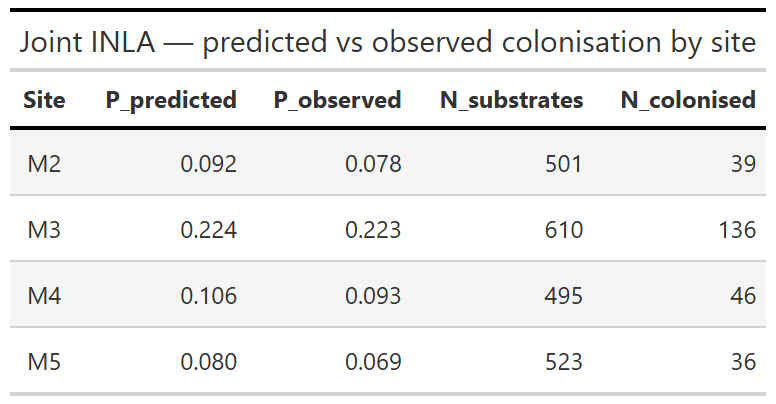
\includegraphics[width=0.6\linewidth,height=\textheight,keepaspectratio]{../02_Displays/Tables/pred_vs_observed_by_site.png}
\end{center}

\textbf{Fixed effects - Process 2 :} Substrate saproxylation stage was
the dominant driver of colonisation probability. Relative to stage 1
(reference), stages 4 and 5 showed large positive effects (β = 2.12
{[}0.09, 4.14{]} and β = 2.61 {[}0.57, 4.65{]} respectively), while
stage 2 was indistinguishable from the reference (β ≈ 0, 95\% CI
spanning zero) and stage 3 showed an intermediate, marginally
significant effect (β = 1.54 {[}-0.50, 3.57{]}). Conifer substrates were
colonised significantly more often than deciduous ones (β = 0.95
{[}0.33, 1.57{]}), consistent with the known preference of
\emph{B.viridis} for softwood species. Substrate diameter had a modest
but significant positive effect (β = 0.51 {[}0.30, 0.71{]}), indicating
that larger logs are more likely to be colonised. Stumps were strongly
disfavoured relative to logs (β = -2.37 {[}-2.92, -1.82{]}).

\begin{center}
\pandocbounded{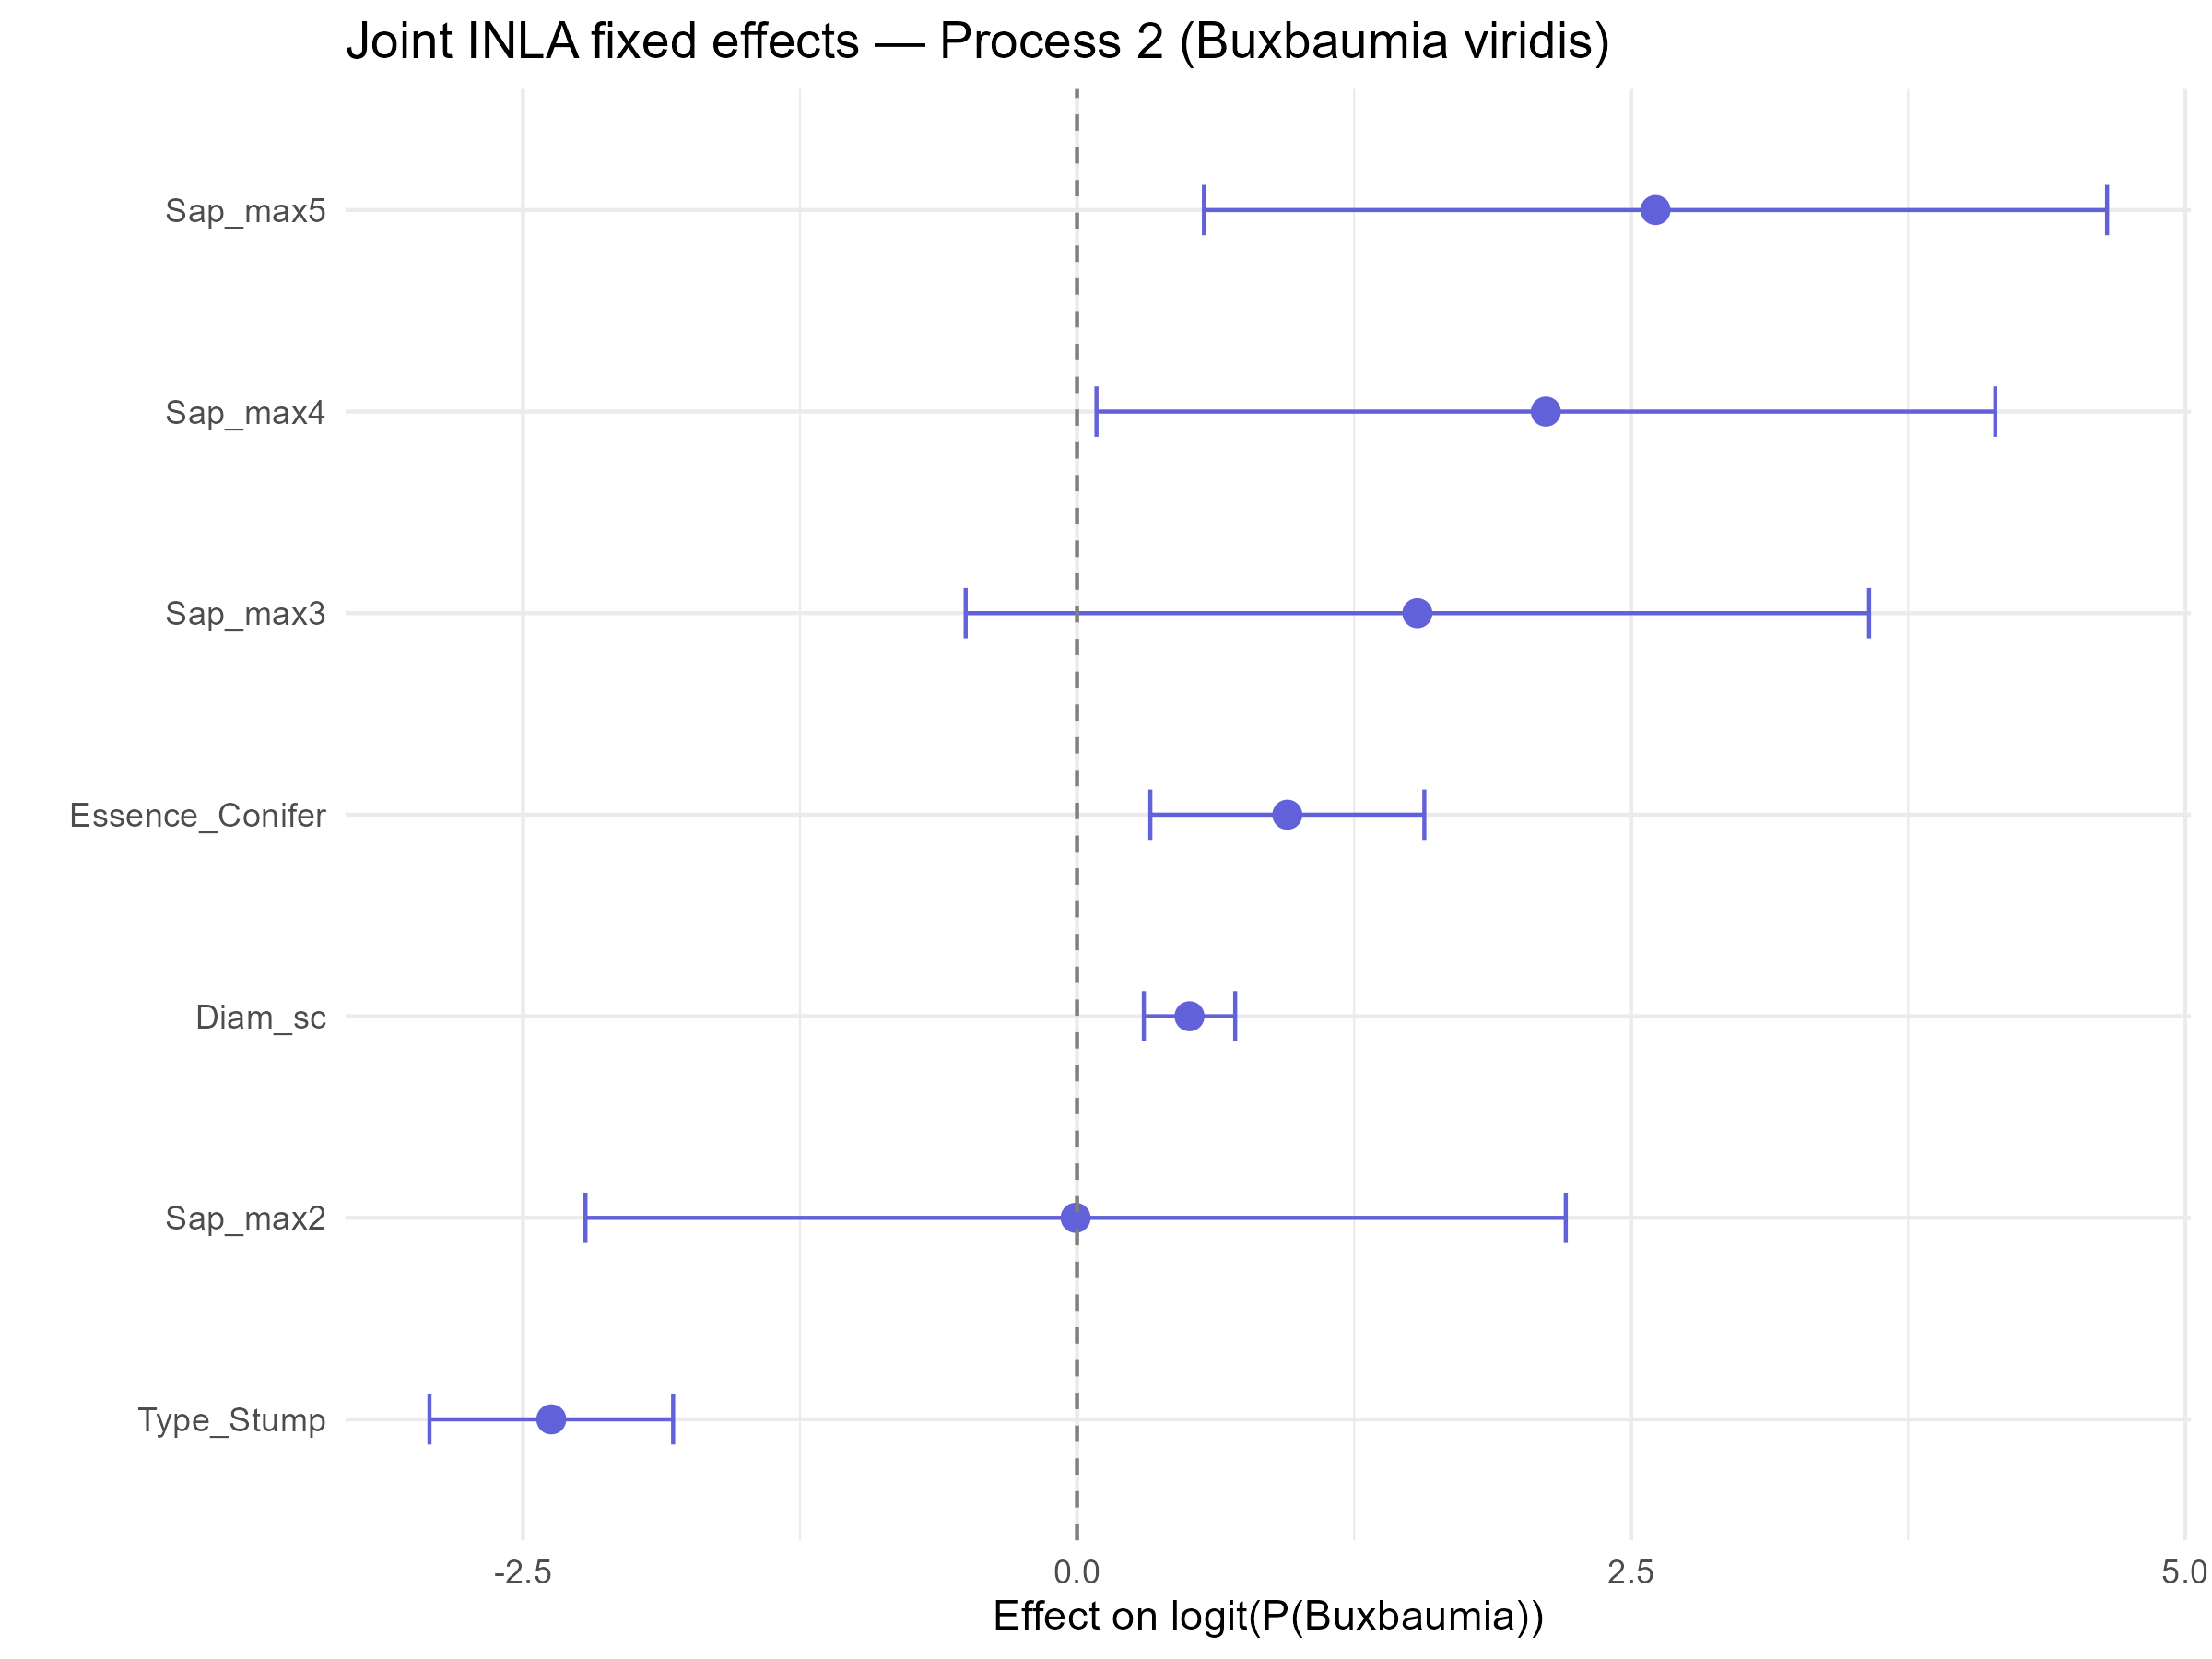
\includegraphics[keepaspectratio]{../02_Displays/Figures/joint_INLA/fixed_effects_P2.png}}
\end{center}

\begin{center}
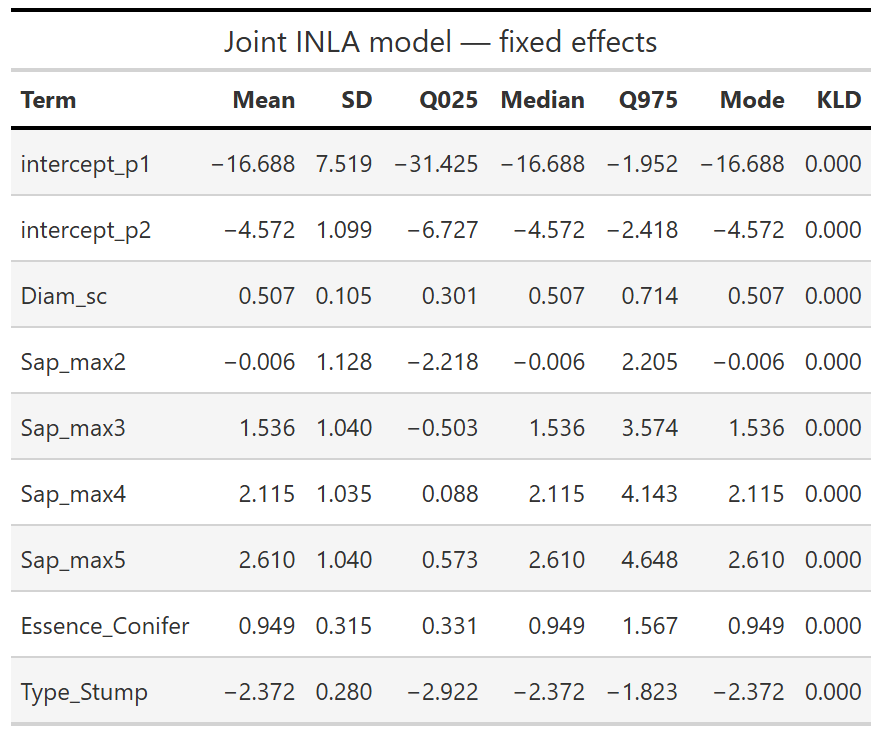
\includegraphics[width=0.6\linewidth,height=\textheight,keepaspectratio]{../02_Displays/Tables/joint_INLA_fixed.png}
\end{center}

\textbf{Spatial fields :} The CWD spatial field \(w_1\) had an estimated
range of 5.5 m {[}0.5--27.4 m{]}, consistent with the metric-scale
clustering identified by the PCF analysis and reflecting the localised
nature of deadwood accumulation around individual dying trees. The
residual \emph{B.viridis} field \(w_2\) operated at a much larger scale,
with an estimated range of 82.9 m {[}49.1--132.9 m{]}, suggesting
broad-scale spatial autocorrelation in colonisation probability that is
not explained by the measured substrate covariates. This residual
structure likely reflects unmeasured environmental gradients, such as
microclimatic variation in humidity, canopy closure or limitations in
\emph{B.viridis} dispersal range operating at the plot scale. The
\(w_2\) maps reveal spatially coherent zones of higher and lower
colonisation probability within each site, which do not correspond to
any single measured covariate, pointing to the existence of site-level
heterogeneity beyond the substrate properties included in the model.

\begin{center}
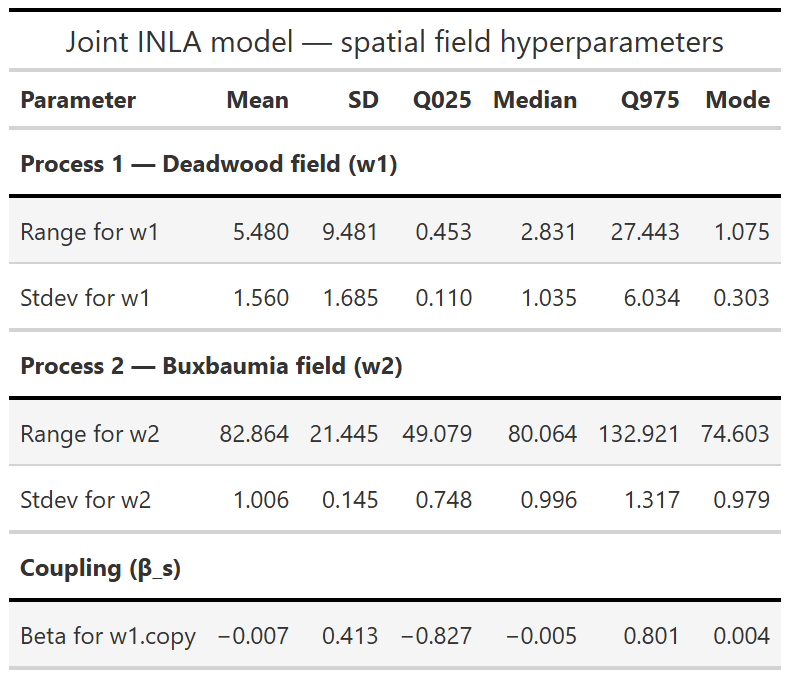
\includegraphics[width=0.6\linewidth,height=\textheight,keepaspectratio]{../02_Displays/Tables/joint_INLA_hyper.png}
\end{center}

\begin{center}
\pandocbounded{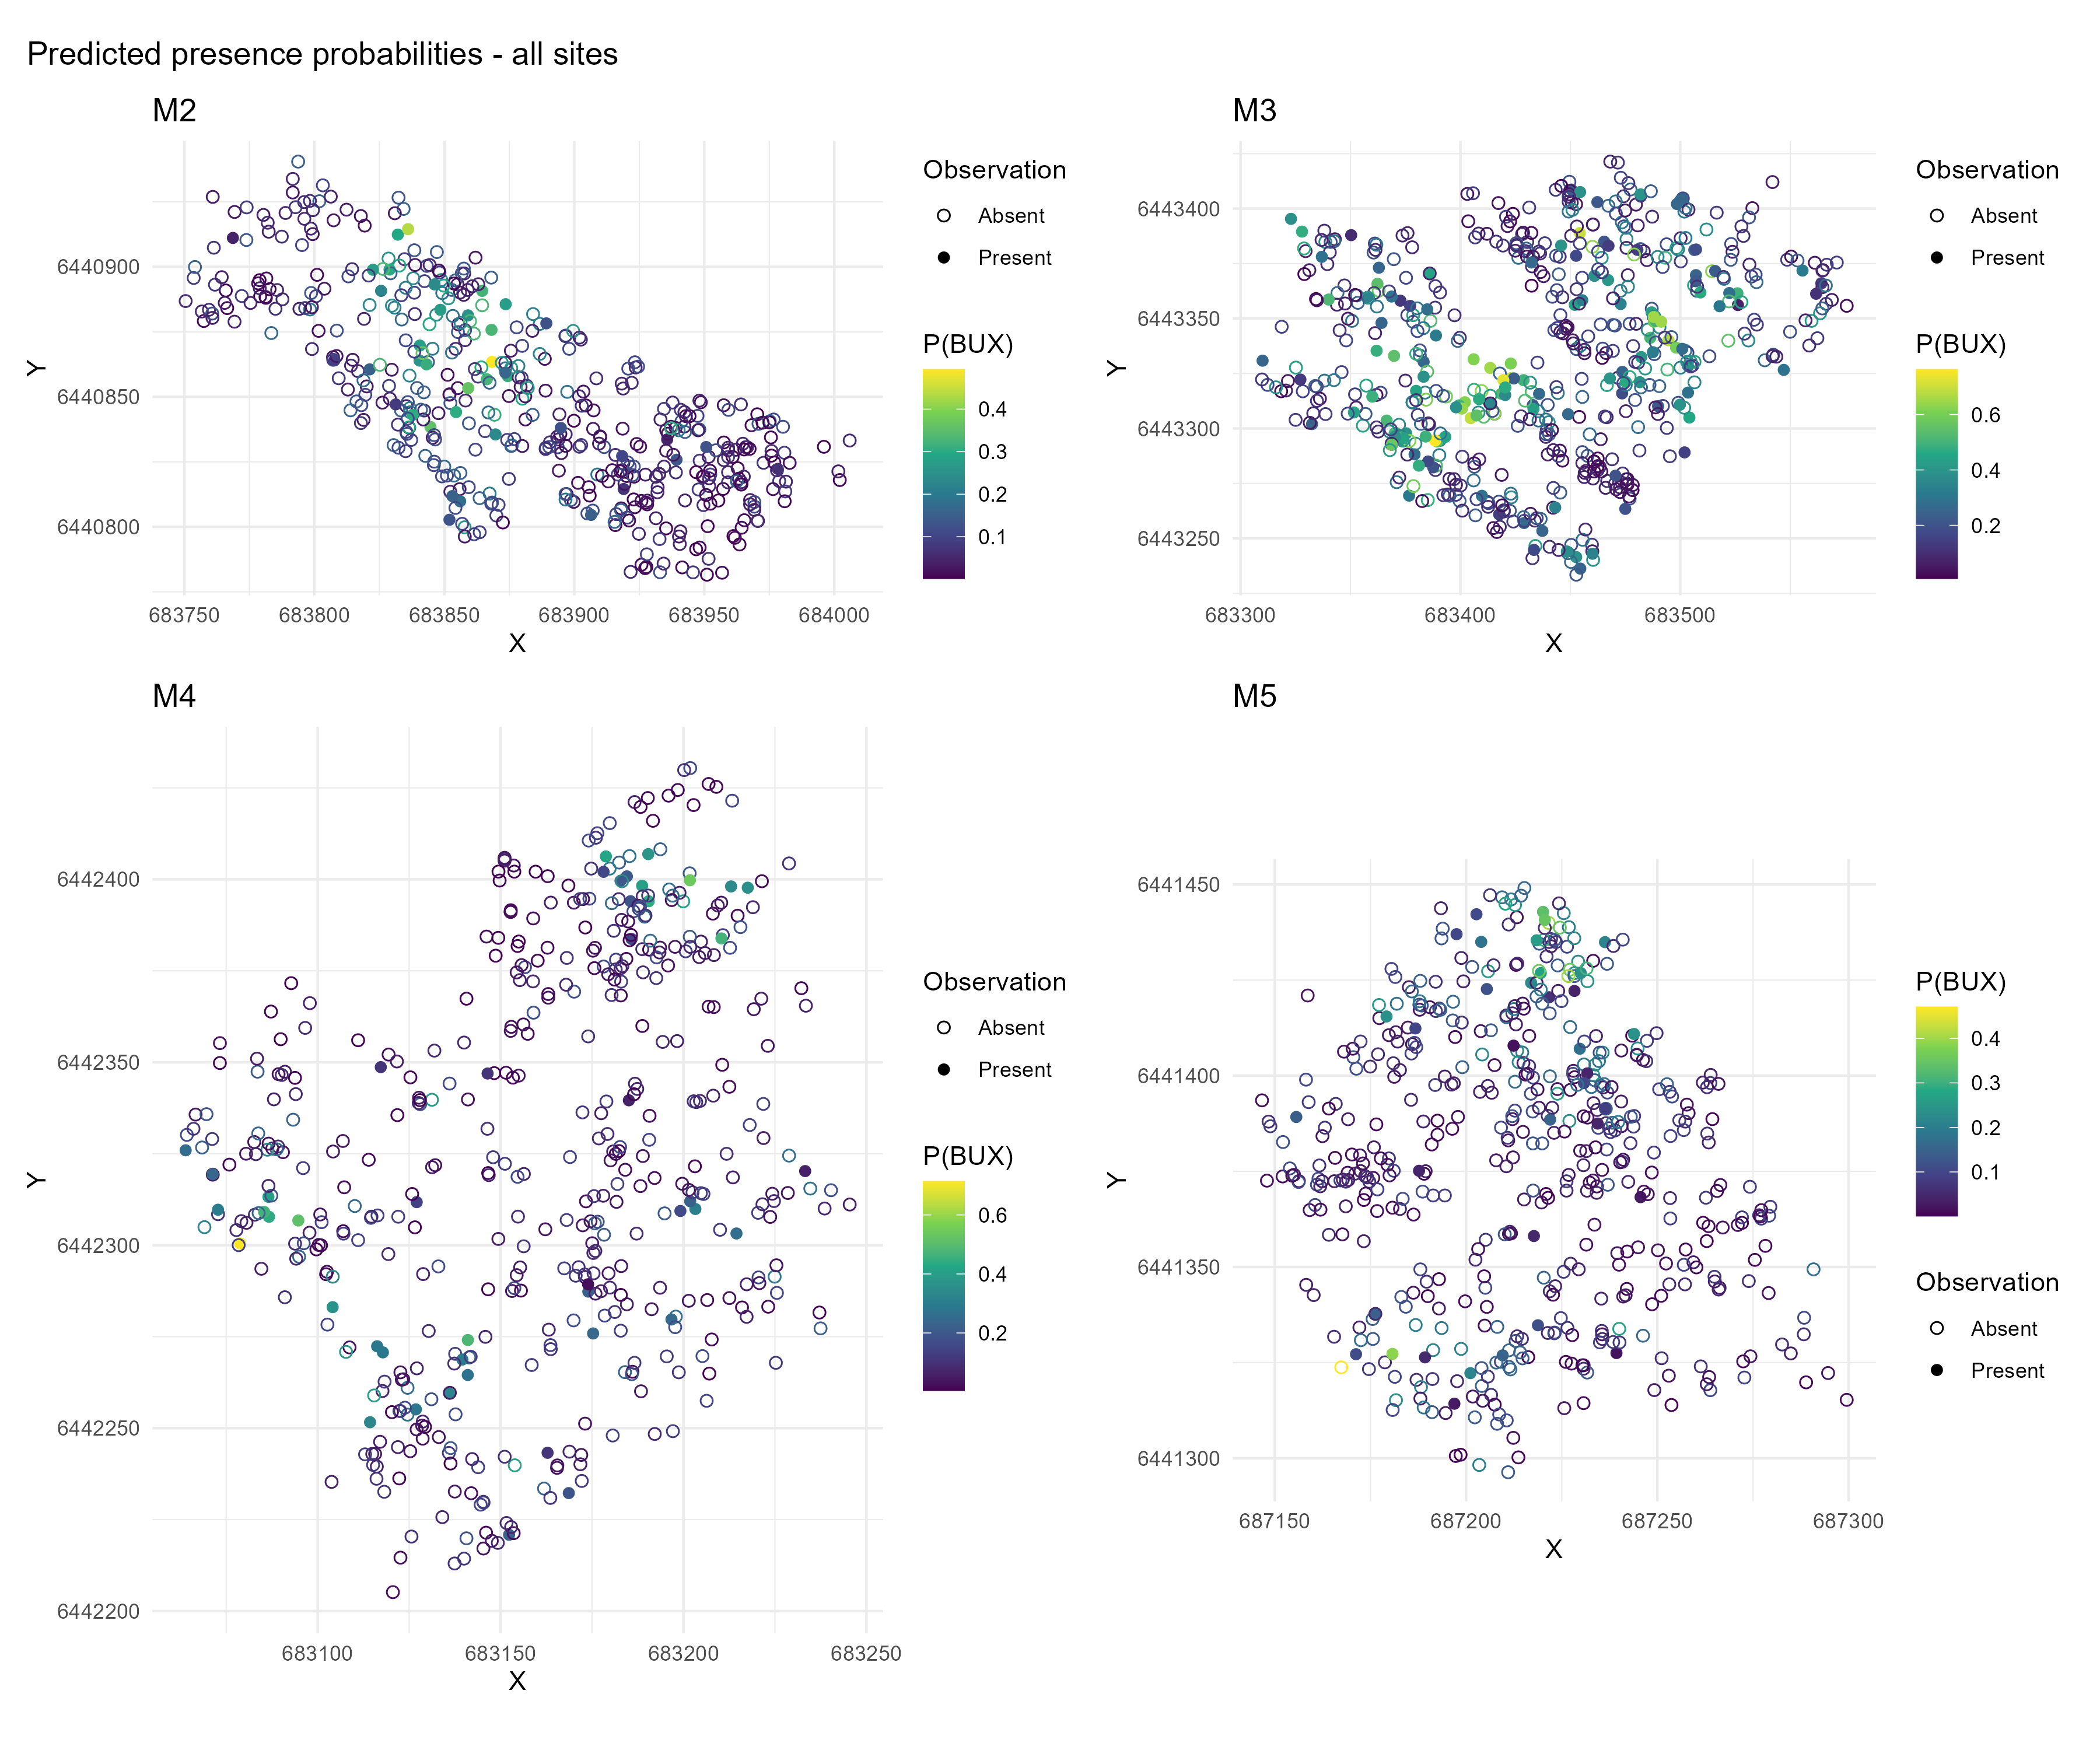
\includegraphics[keepaspectratio]{../02_Displays/Figures/joint_INLA/pred_all_sites.png}}
\end{center}

\textbf{Coupling coefficient β\_s :} The posterior distribution of the
coupling coefficient \(β_s\) was centred near zero (mean = -0.007, 95\%
CI {[}-0.827, 0.801{]}, P(\(β_s\) \textgreater{} 0) = 0.495), providing
no evidence that areas of high deadwood density exert any additional
effect on colonisation probability beyond what is already captured by
individual substrate covariates. This null result is ecologically
informative : once substrate quality (saproxylation, diameter, species,
type) is controlled for, the local spatial density of deadwood does not
influence colonisation. This confirms that \emph{B.viridis} responds to
substrate-level properties rather than to neighbourhood deadwood
abundance.

\begin{center}
\pandocbounded{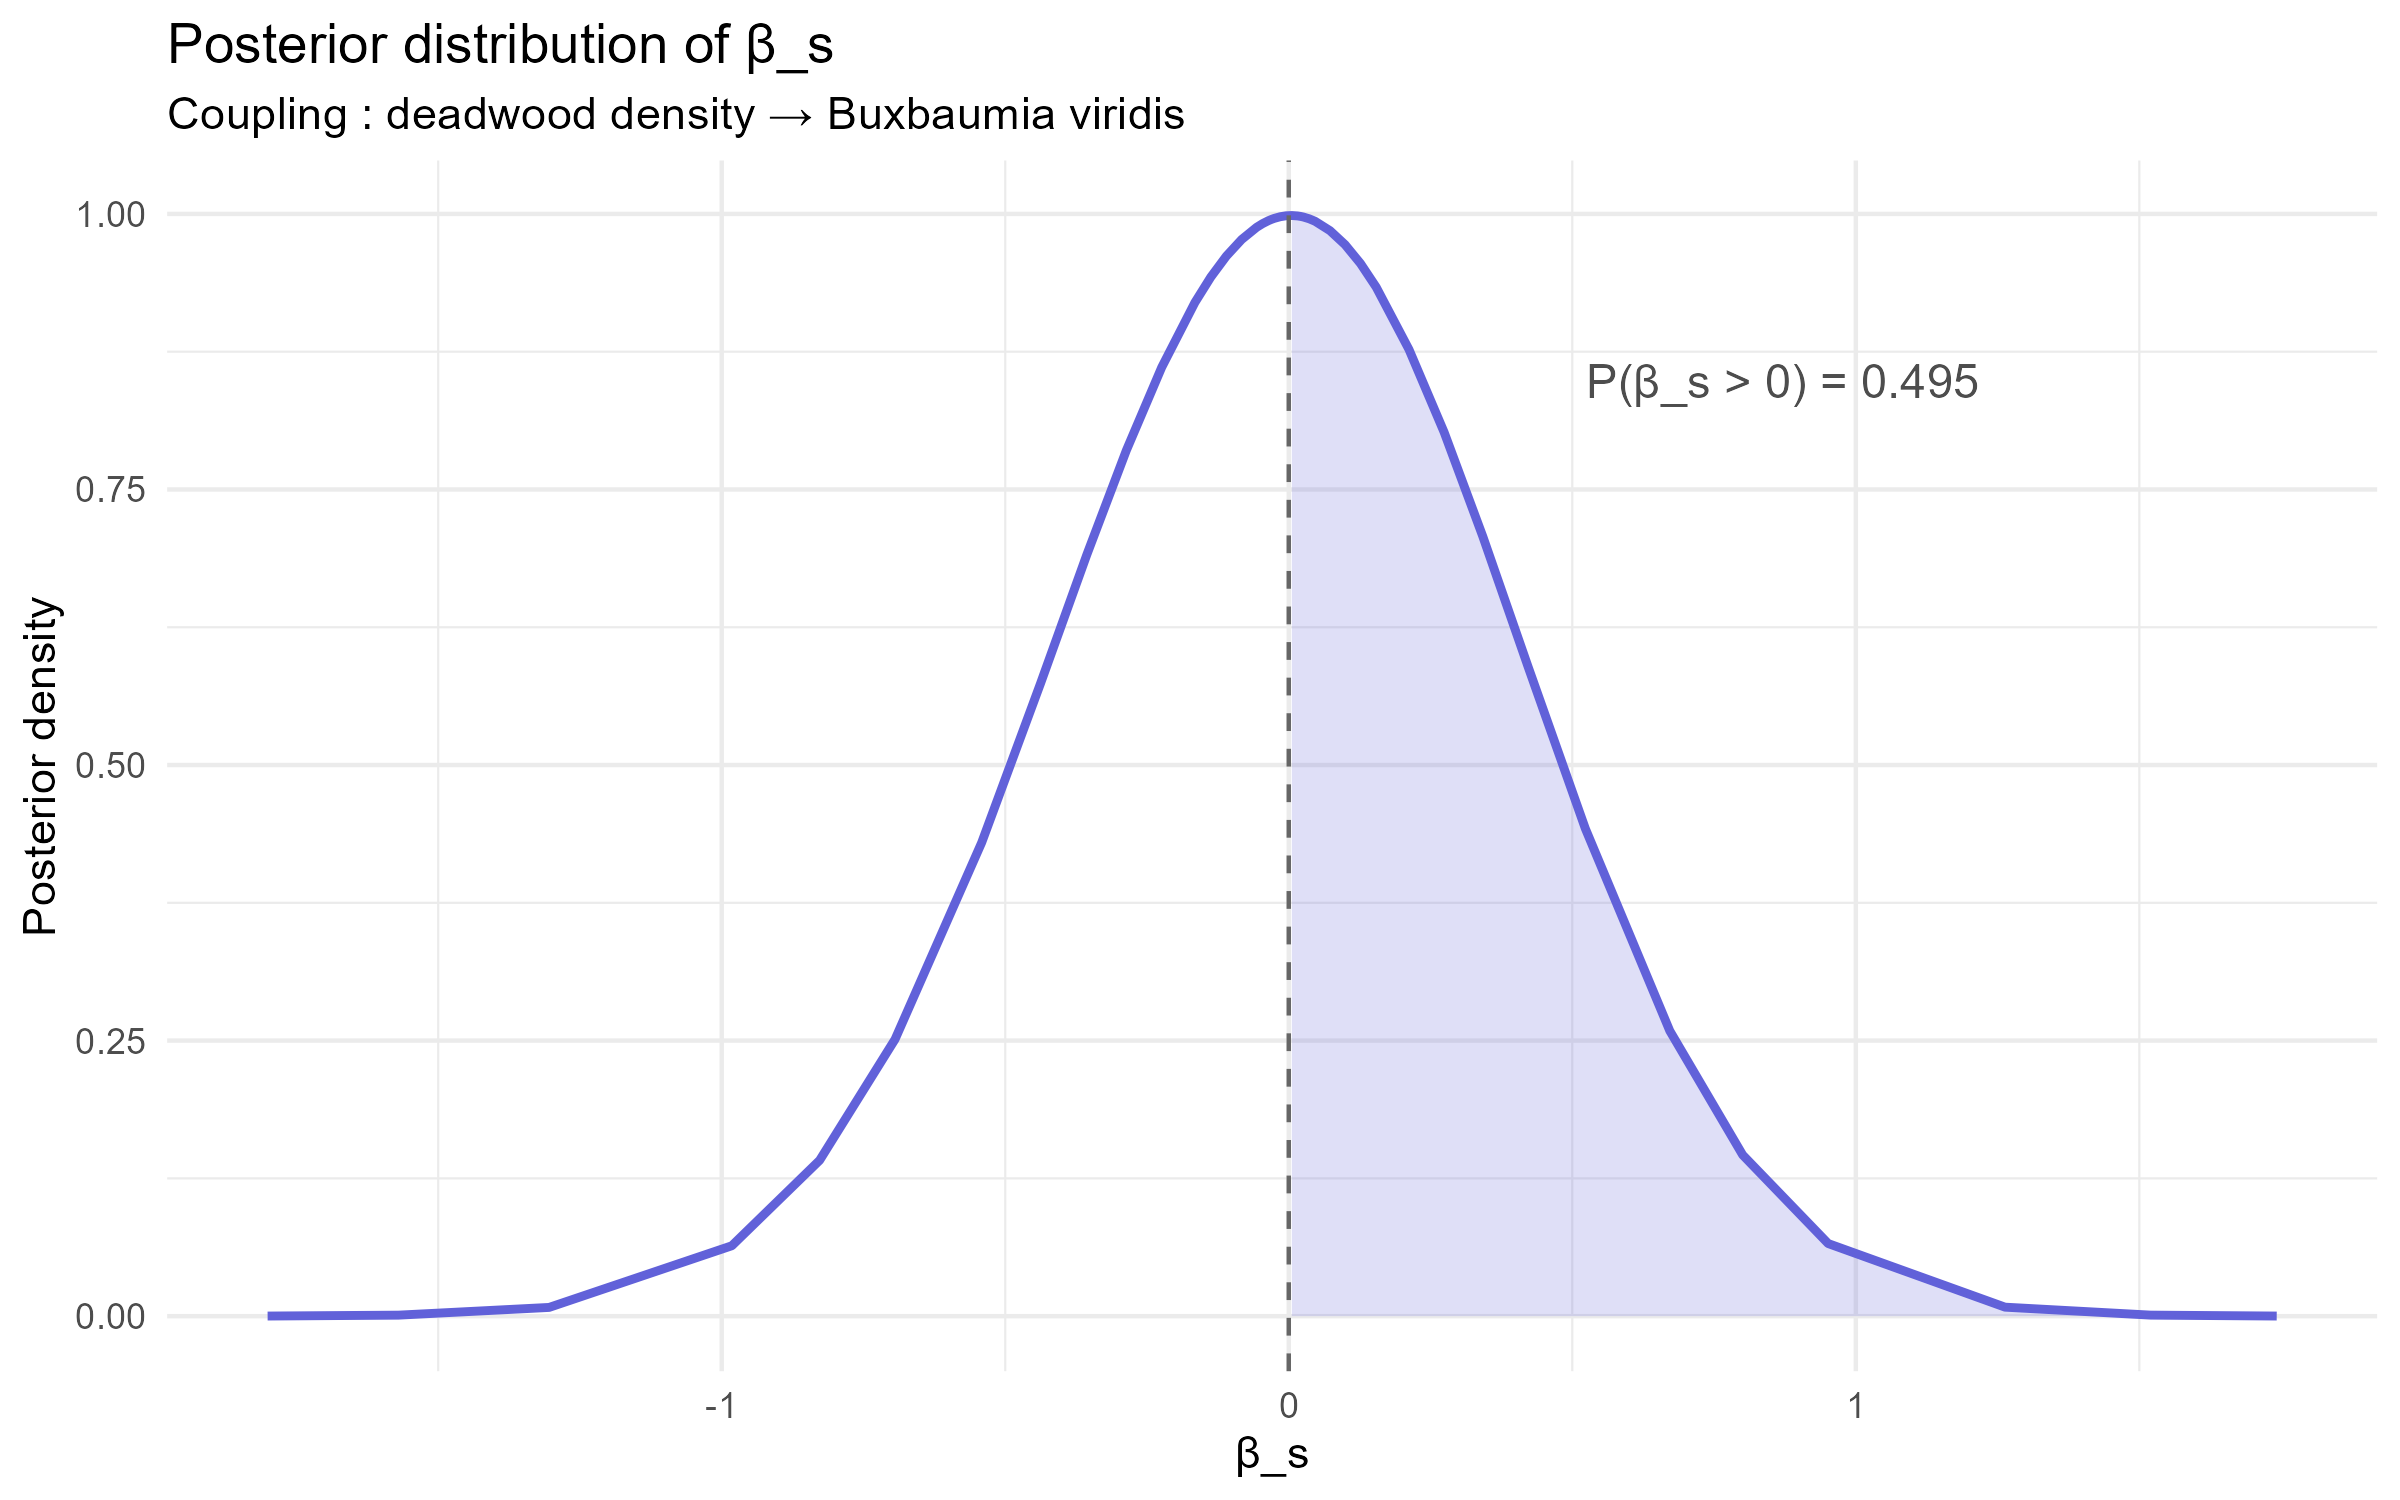
\includegraphics[keepaspectratio]{../02_Displays/Figures/joint_INLA/beta_s_posterior.png}}
\end{center}

\textbf{Model fit and calibration :} The ROC curve yielded an AUC of
0.856, indicating good overall discrimination. The PIT histogram,
however, reveals a strong right-skewed distribution concentrated near 1,
indicating that the model is overconfident for a large proportion of
observations, systematically assigning low predicted probabilities to
uncolonised substrates, which is formally correct but masks poor
resolution for the positive class. This right-skewed pattern is however
expected in the context of rare species distribution modelling : when
presence events are scarce relative to absences, the model correctly
assigns low predicted probabilities to the vast majority of
observations, which mechanically concentrates PIT values near 1. This
pattern therefore reflects the structural imbalance of the data rather
than a genuine calibration failure, and should not be interpreted as a
model deficiency (Jeliazkov \emph{et al.} 2022). The distribution of
predicted probabilities by site confirms this pattern : colonised and
uncolonized substrates partially overlap in predicted probability space,
particularly at sites with low colonisation rates (M2, M4, M5), where
the model struggles to distinguish positive cases from the bulk of
uncolonised substrates.

\begin{center}
\pandocbounded{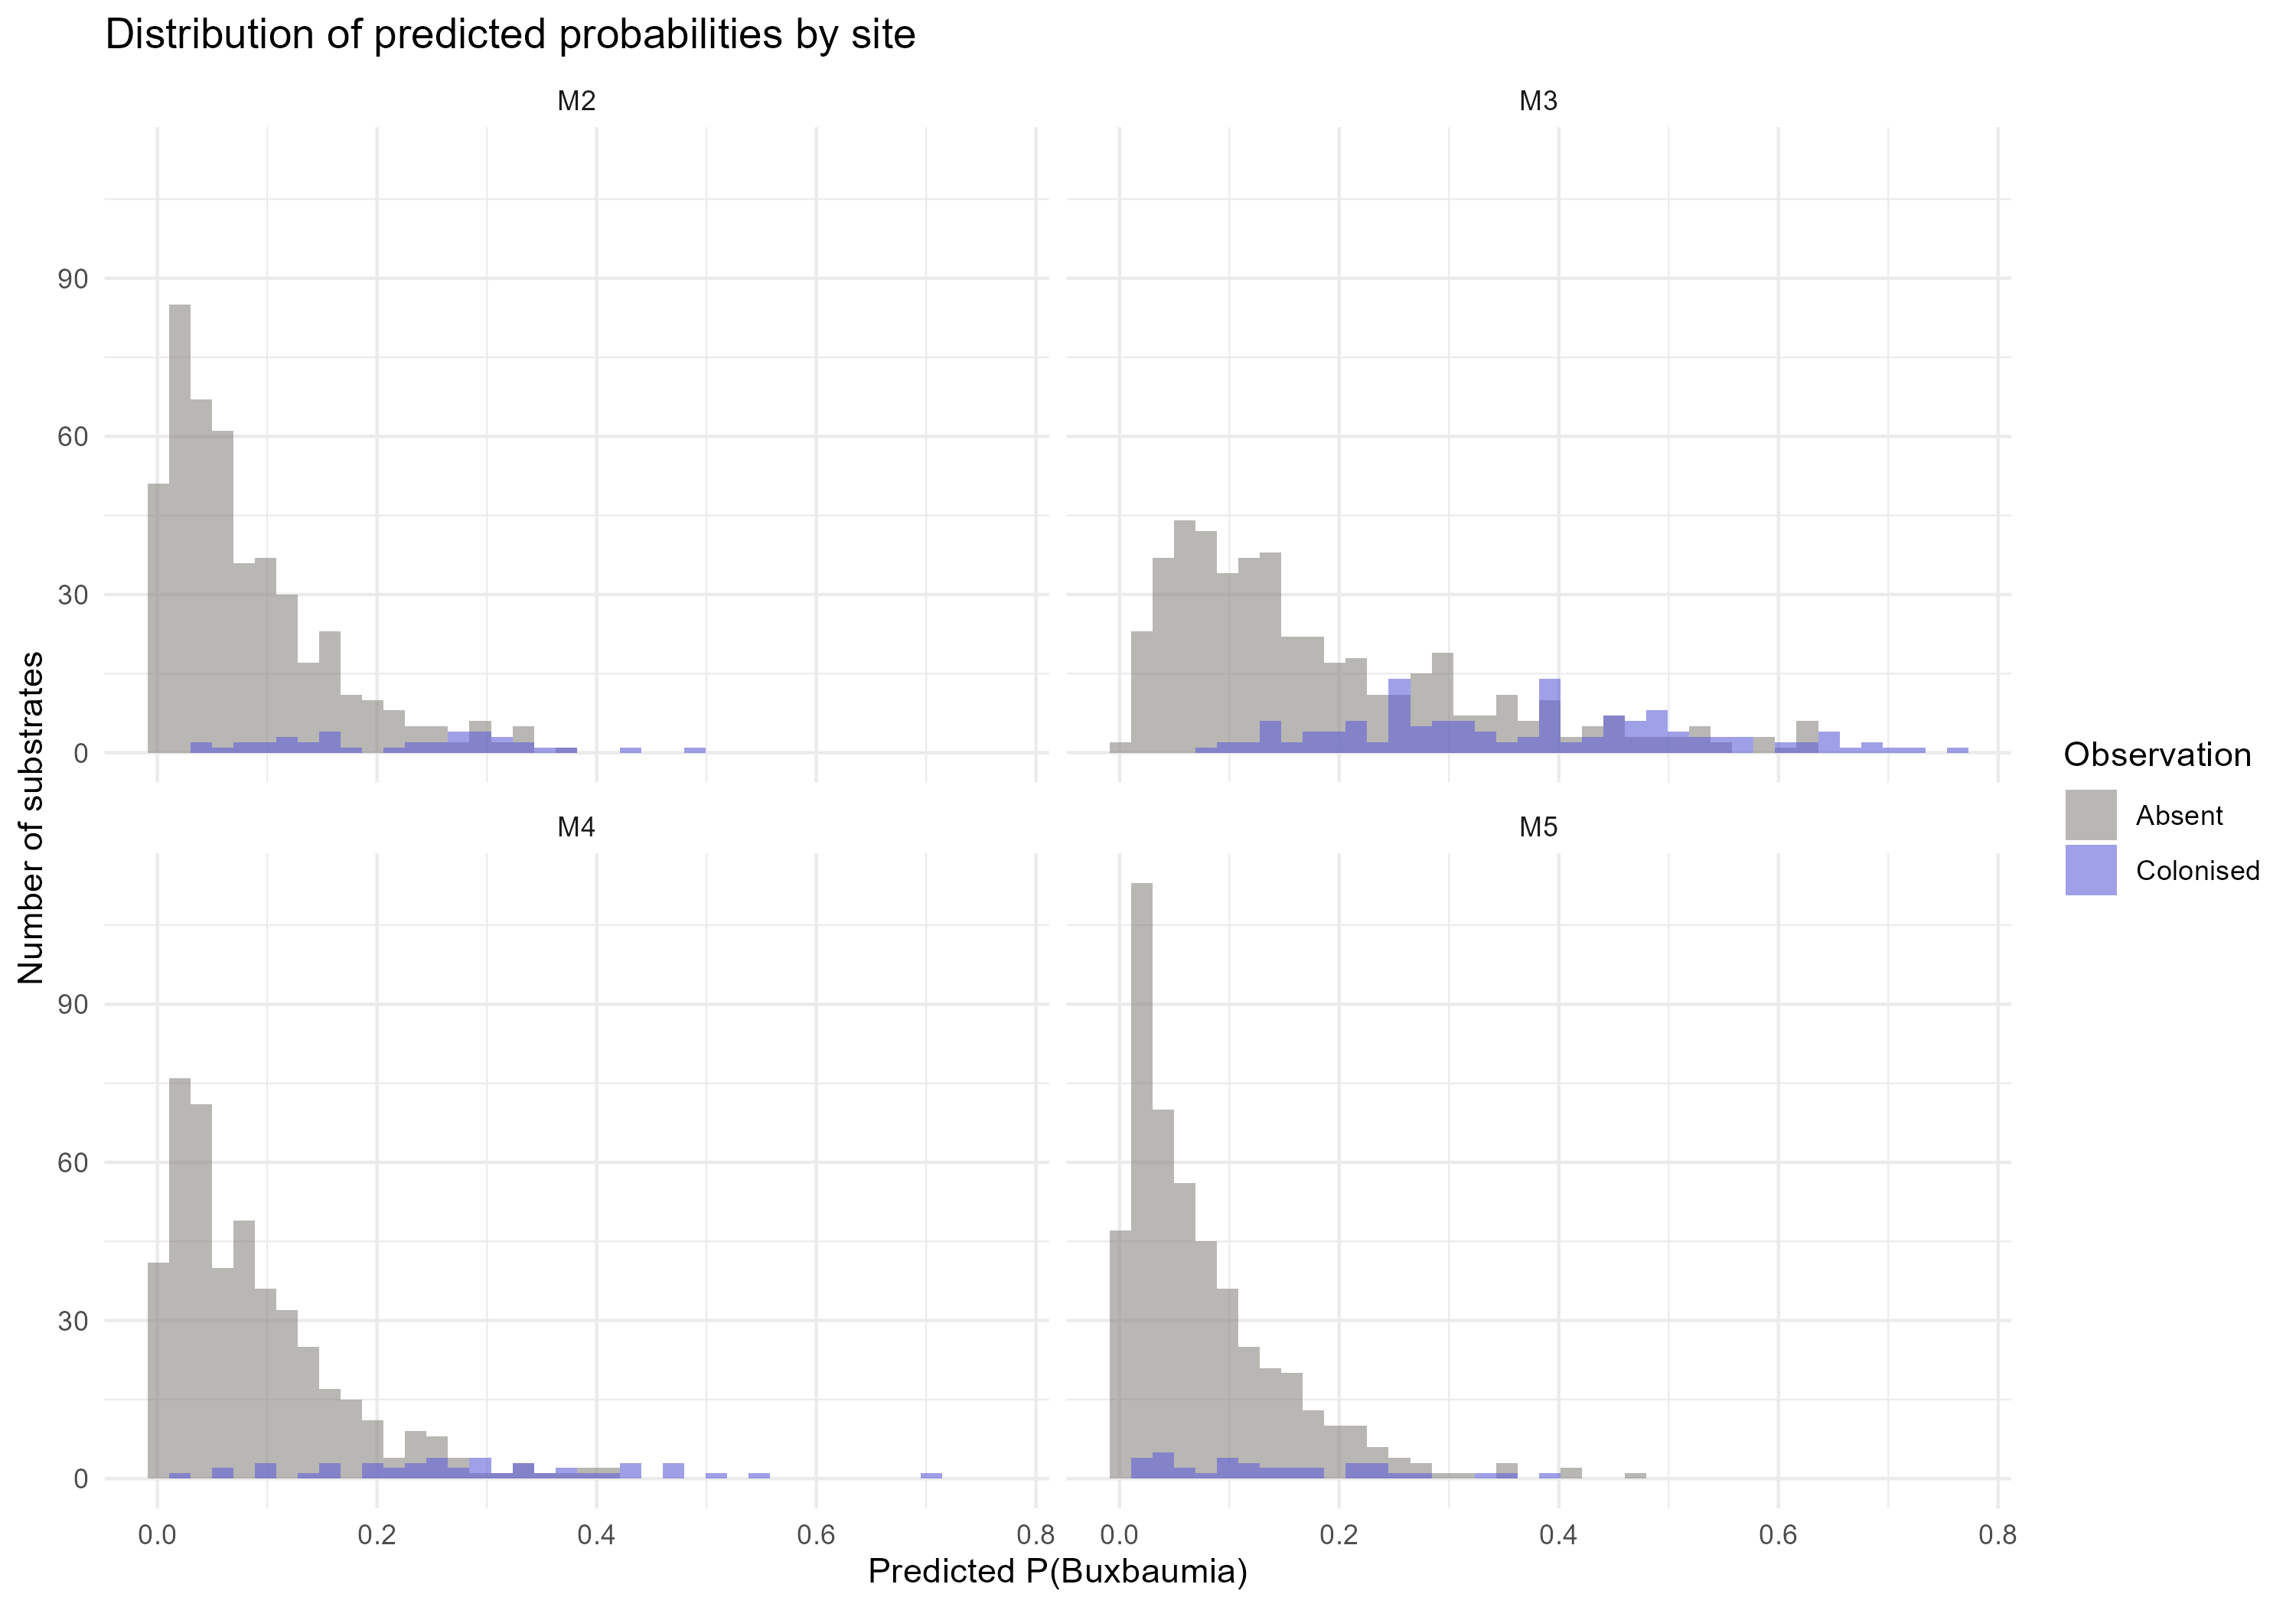
\includegraphics[keepaspectratio]{../02_Displays/Figures/joint_INLA/predictions_distribution.png}}
\end{center}

\begin{center}
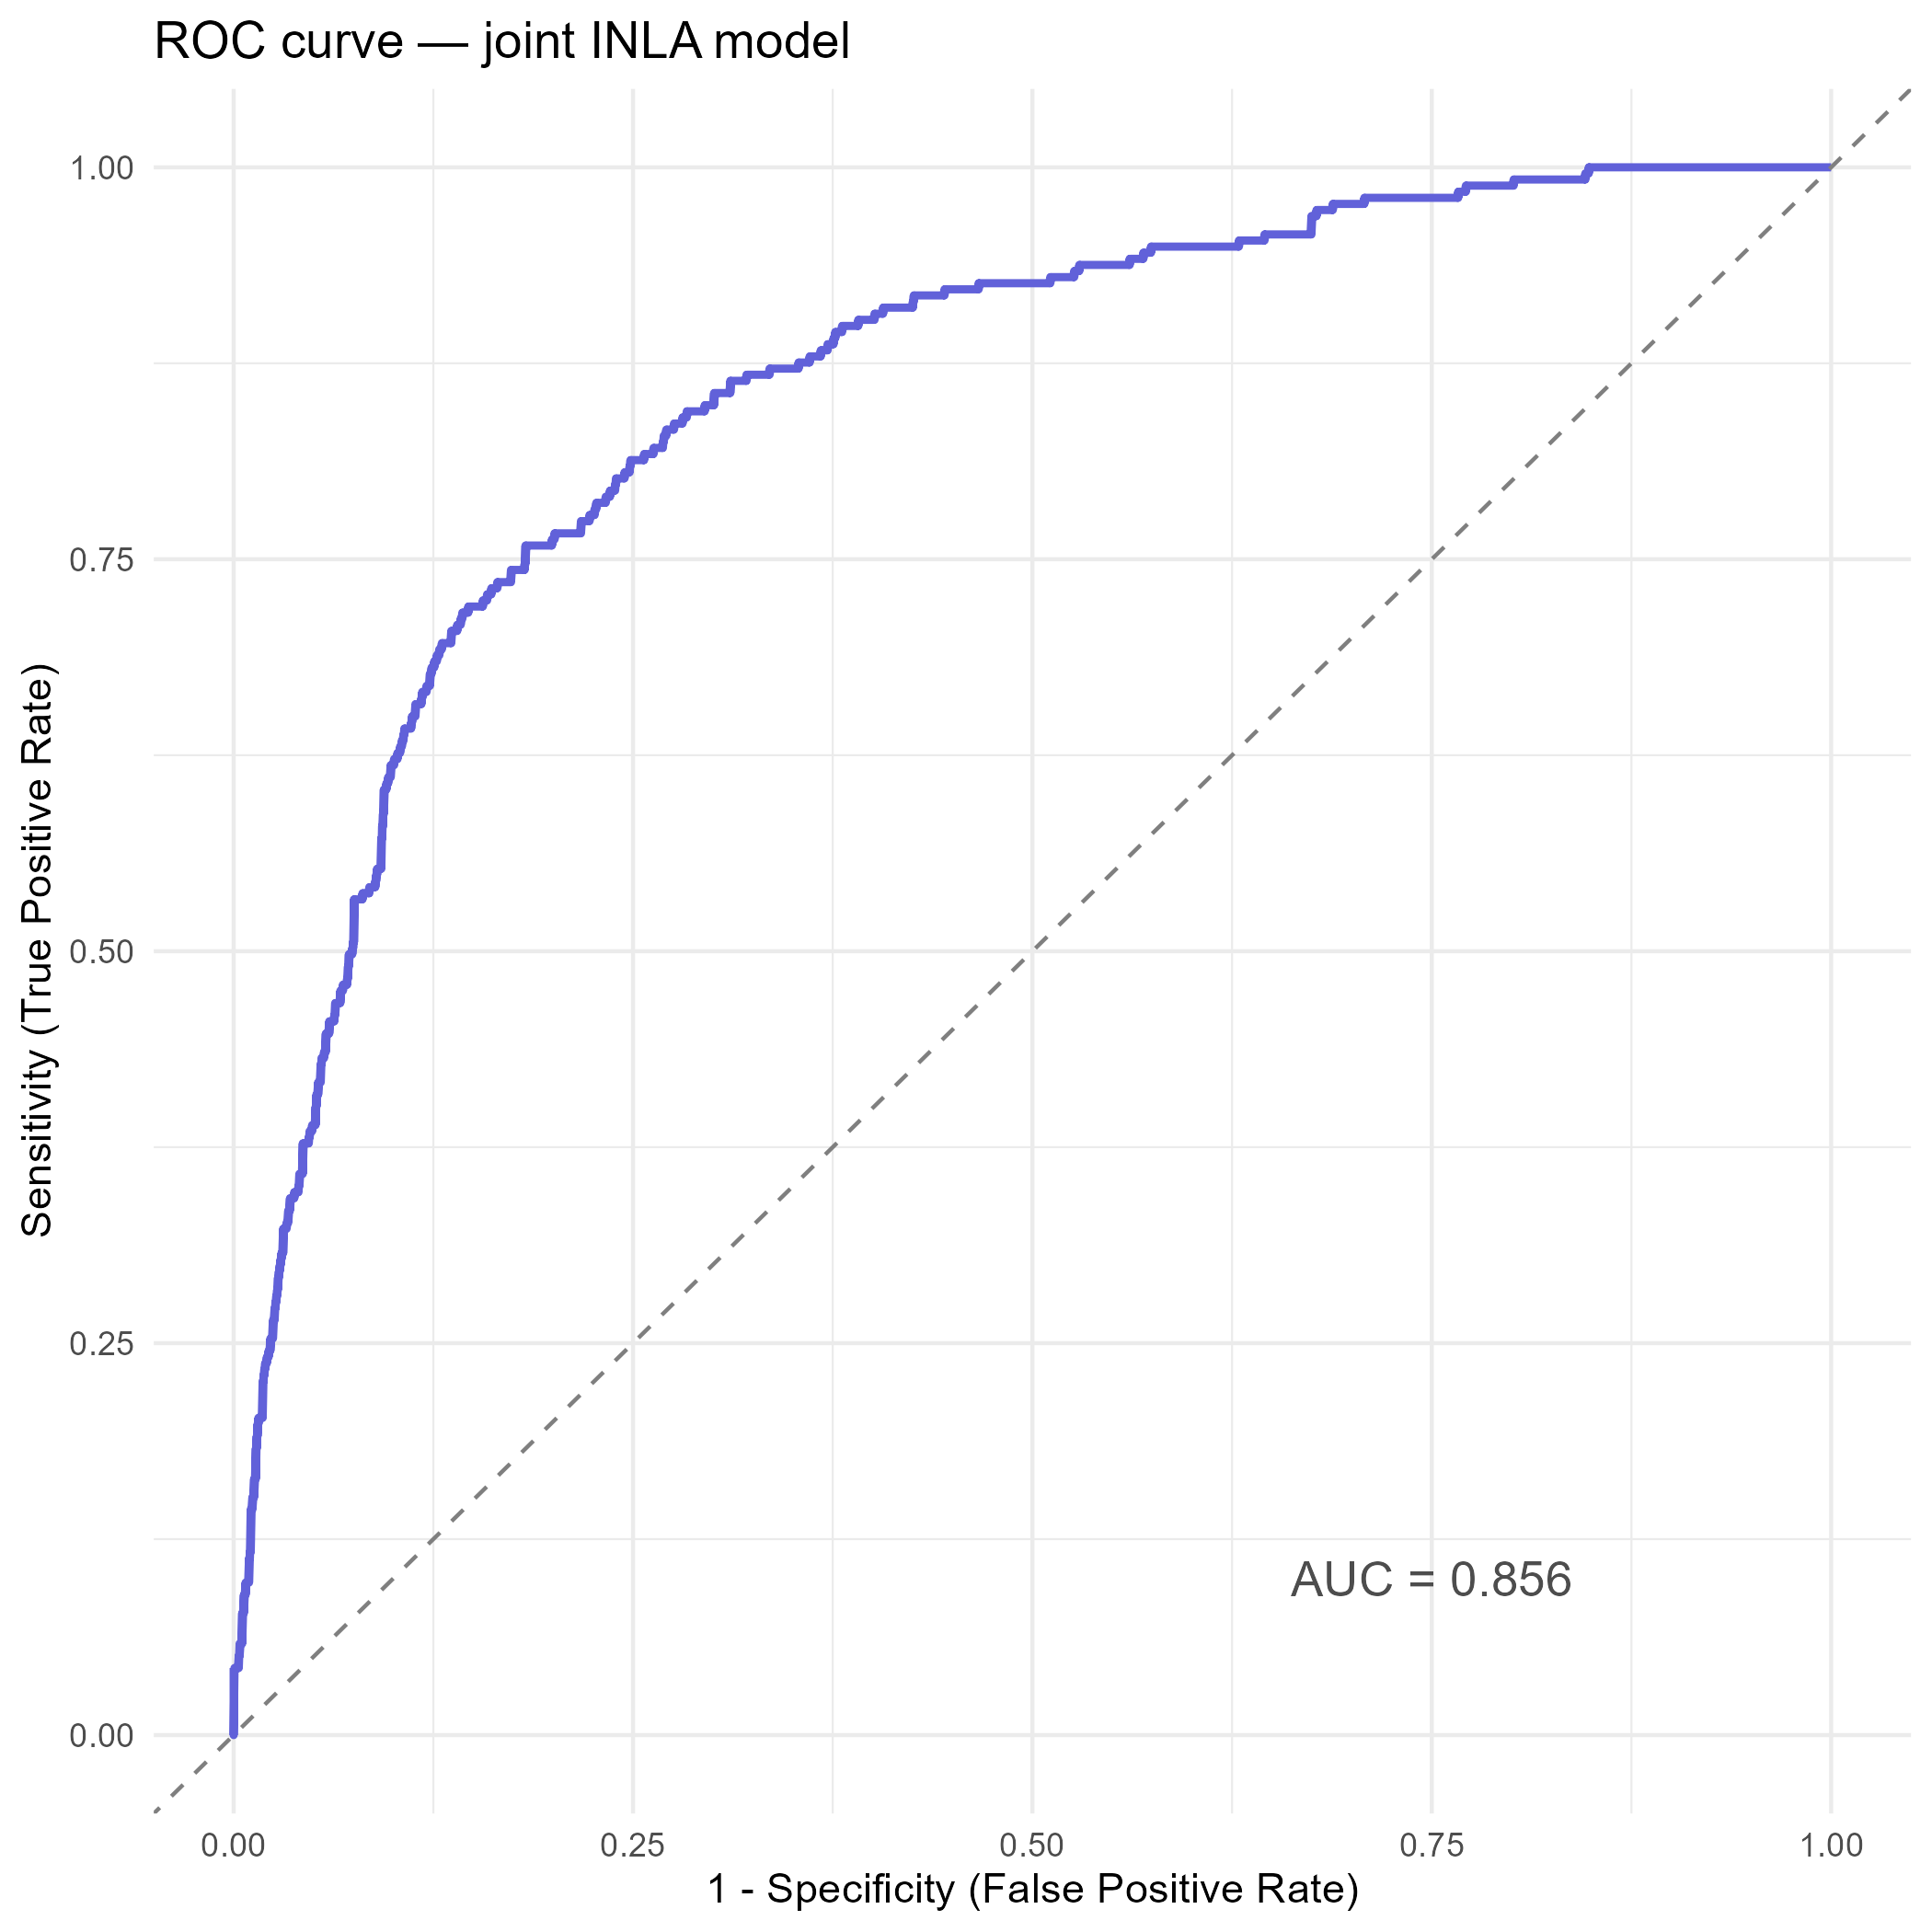
\includegraphics[width=0.7\linewidth,height=\textheight,keepaspectratio]{../02_Displays/Figures/joint_INLA/ROC_curve.png}
\end{center}

\begin{center}
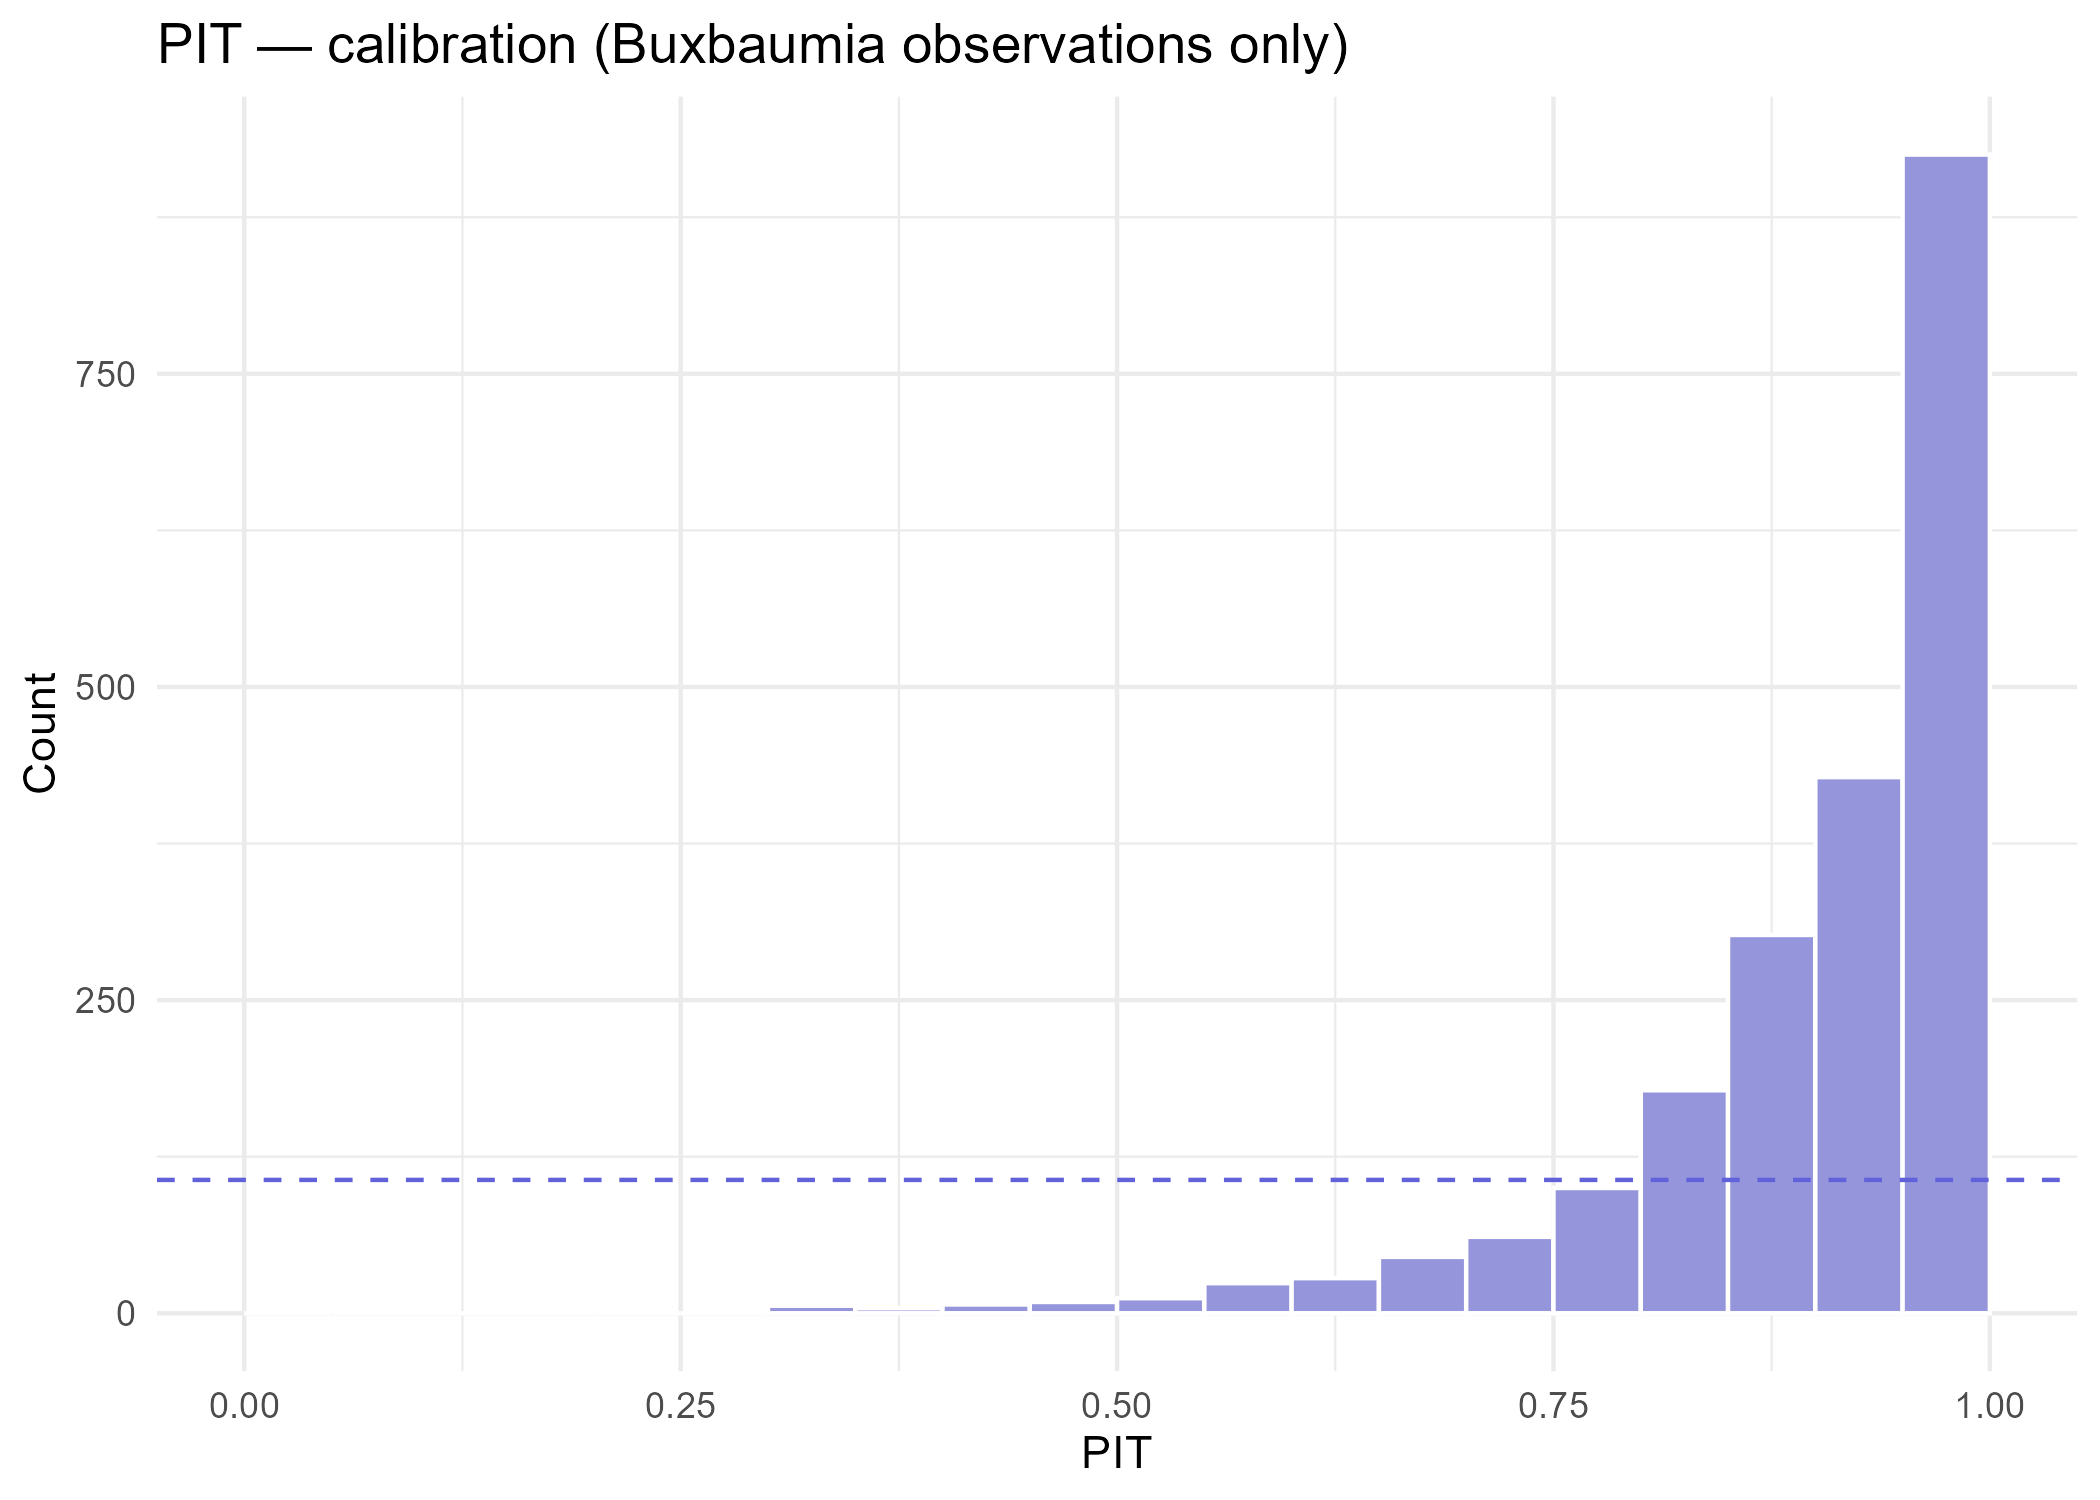
\includegraphics[width=0.8\linewidth,height=\textheight,keepaspectratio]{../02_Displays/Figures/joint_INLA/PIT_calibration.png}
\end{center}

\subsubsection{Null Trend Verification}\label{null-trend-verification}

This result \(β_s\) ≈ 0 may appear surprising, both because it
contradicts the positive effect of local deadwood density observed in
the PPM, and because it challenges the hypothesis, supported in the
literature, that dense deadwood aggregations create favourable
microclimatic conditions or facilitate short-distance spore dispersal.
To verify that this result does not reflect a modelling artefact, such
as over-absorption of the density signal by the residual field \(w_2\)
or prior sensitivity, we conducted an independent non-parametric
verification. For each substrate, the local deadwood density was
computed as the number of neighbouring substrates within a 10 m radius,
excluding the focal point itself. The correlation between this
neighbourhood density index and colonisation status (P\_BUX) was then
assessed using Spearman's rank correlation coefficient, both globally
across all sites and independently within each site. This approach is
entirely model-free and makes no assumption about spatial structure or
covariate effects, providing a direct empirical test of whether
substrates located in denser deadwood neighbourhoods are more frequently
colonised than isolated ones.

\textbf{Results :} The Spearman correlation test confirmed the absence
of any meaningful association between local deadwood density and
colonisation status. At the global level, the correlation was negligible
and non-significant (\(ρ\) = -0.022, p = 0.310, n = 2129). Site-level
results were equally uninformative : correlations ranged from \(ρ\) =
-0.029 (M4) to \(ρ\) = 0.090 (M2), and were non-significant at three out
of four sites. The only marginally significant result, observed at M2
(\(ρ\) = 0.090, p = 0.044), was of negligible effect size and should be
interpreted with caution given the large number of tied ranks inherent
to a binary response variable, which prevented exact p-value
computation. Taken together, these model-free results are fully
consistent with the \(β_s\) ≈ 0 estimate from the joint INLA model, and
confirm that local deadwood density carries no detectable signal for
\emph{B.viridis} colonisation at the spatial scale investigated. The
species appears to select substrates on the basis of their intrinsic
properties rather than their spatial context within the deadwood
network.

\begin{center}
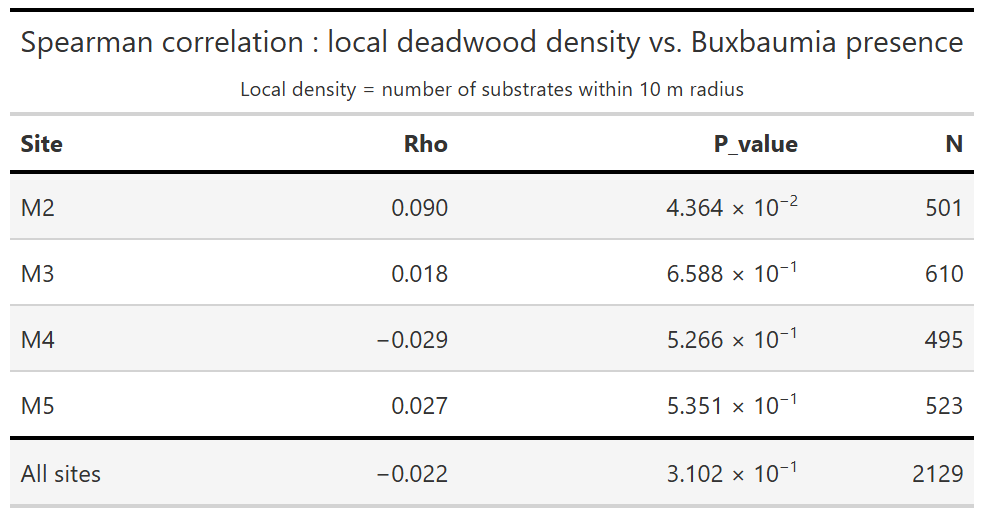
\includegraphics[width=0.75\linewidth,height=\textheight,keepaspectratio]{../02_Displays/Tables/spearman_coupling.png}
\end{center}

\subsubsection{Spatial block
cross-validation}\label{spatial-block-cross-validation}

The predictive performance of the joint INLA model was assessed using a
repeated spatial block holdout procedure, designed to account for the
spatial autocorrelation structure of the data. Standard random
cross-validation is inappropriate in spatially structured datasets
because training and test observations drawn from nearby locations share
autocorrelated residuals, leading to optimistic performance estimates
that do not reflect genuine predictive ability at unobserved locations
(Roberts \emph{et al.}, 2017).

The spatial block cross-validation procedure follows the methodology
described in J.Papaïx, J-Y.Barnagaud \emph{et al.} (unpublished) :
Spatial analysis of the wildlife roadkill risk at a regional scale.At
each of the 100 replicates, one random point was drawn per site, and all
substrates located within a 40 m radius of that point were assigned to
the test set. This exclusion radius was chosen to exceed the estimated
range of the residual \emph{B.viridis} spatial field \(w_2\)
(\textasciitilde82 m posterior mean), ensuring that test observations
are spatially decoupled from the training set and that the model cannot
exploit local autocorrelation to inflate predictive scores. The model
was then re-estimated from scratch on the remaining training data using
the same joint INLA specification (LGCP + Binomial, shared field
\(w_1\), residual field \(w_2\)), with the \emph{ccd} integration
strategy for full accuracy. Predictions on the test set were computed
from fixed effects only, without extrapolating the spatial random fields
to held-out locations, which would artificially borrow strength from the
training spatial structure.

Predictive discrimination was quantified using the Area Under the ROC
Curve (AUC), computed both globally across all sites and independently
within each site. Replicates yielding fewer than five test observations
or a degenerate response (all absences or all presences in the test set)
were discarded.

\begin{tcolorbox}[enhanced jigsaw, breakable, colback=white, opacityback=0, bottomtitle=1mm, arc=.35mm, rightrule=.15mm, colbacktitle=quarto-callout-note-color!10!white, titlerule=0mm, colframe=quarto-callout-note-color-frame, toprule=.15mm, opacitybacktitle=0.6, coltitle=black, left=2mm, bottomrule=.15mm, leftrule=.75mm, toptitle=1mm, title=\textcolor{quarto-callout-note-color}{\faInfo}\hspace{0.5em}{NB}]

\emph{Not yet executed, awaiting confirmation of the relevance of the
model structure}

\end{tcolorbox}

\textbf{INLA joint model validation function code}

\begin{Shaded}
\begin{Highlighting}[]
\CommentTok{\# {-}{-}{-}{-}{-}{-}{-}{-}{-}{-}{-}{-}{-}{-}{-}{-}{-}{-}{-}{-}{-}{-}{-}{-}{-}{-}{-}{-}{-}{-}{-}{-}{-}{-}{-}{-}{-}{-}{-}{-}{-}{-}{-}{-}{-}{-}{-}{-}{-}{-}{-}{-}{-}{-}{-}{-}{-}{-}{-}{-}{-}{-}{-}{-}{-}{-}{-}{-}{-}{-}{-}{-}{-}{-}{-}{-}{-}}
\CommentTok{\# run\_parallel\_cv : Parallelised spatial block cross{-}validation}
\CommentTok{\#}
\CommentTok{\# Evaluates the predictive performance of the joint INLA model using repeated}
\CommentTok{\# spatial block holdout. At each replicate, one random point per site is drawn}
\CommentTok{\# and all substrates within a given radius are excluded from training.}
\CommentTok{\# The model is re{-}fitted on the remaining data and predictions are made on the}
\CommentTok{\# test set using fixed effects only (no spatial field extrapolation).}
\CommentTok{\#}
\CommentTok{\# Arguments:}
\CommentTok{\#   res : output object from fun\_joint\_inla()}
\CommentTok{\#   n\_rep : number of cross{-}validation replicates}
\CommentTok{\#   radius : exclusion radius in metres around the holdout point}
\CommentTok{\#   n\_cores : number of parallel cores}
\CommentTok{\#   error\_handling : foreach error handling }
\CommentTok{\#                    {-}\textgreater{} "remove" (skip) or "pass" (return error)}
\CommentTok{\#}
\CommentTok{\# Returns a data frame with one row per valid replicate :}
\CommentTok{\#   $rep : replicate index}
\CommentTok{\#   $n\_test : number of test observations}
\CommentTok{\#   $n\_train : number of training observations}
\CommentTok{\#   $auc : global AUC}
\CommentTok{\#   $auc\_M2 ... $auc\_M5 : per{-}site AUC}
\CommentTok{\# {-}{-}{-}{-}{-}{-}{-}{-}{-}{-}{-}{-}{-}{-}{-}{-}{-}{-}{-}{-}{-}{-}{-}{-}{-}{-}{-}{-}{-}{-}{-}{-}{-}{-}{-}{-}{-}{-}{-}{-}{-}{-}{-}{-}{-}{-}{-}{-}{-}{-}{-}{-}{-}{-}{-}{-}{-}{-}{-}{-}{-}{-}{-}{-}{-}{-}{-}{-}{-}{-}{-}{-}{-}{-}{-}{-}{-}}
\NormalTok{run\_parallel\_cv }\OtherTok{\textless{}{-}} \ControlFlowTok{function}\NormalTok{(res, }\AttributeTok{n\_rep =} \DecValTok{100}\NormalTok{, }\AttributeTok{radius =} \DecValTok{40}\NormalTok{, }\AttributeTok{n\_cores =} \DecValTok{9}\NormalTok{,}
                            \AttributeTok{error\_handling =} \StringTok{"remove"}\NormalTok{) \{}
\NormalTok{  df\_full }\OtherTok{\textless{}{-}}\NormalTok{ res}\SpecialCharTok{$}\NormalTok{data}
\NormalTok{  df\_full}\SpecialCharTok{$}\NormalTok{Site }\OtherTok{\textless{}{-}} \FunctionTok{factor}\NormalTok{(df\_full}\SpecialCharTok{$}\NormalTok{Site)}
\NormalTok{  sites }\OtherTok{\textless{}{-}} \FunctionTok{levels}\NormalTok{(df\_full}\SpecialCharTok{$}\NormalTok{Site)}

  \FunctionTok{message}\NormalTok{(}\FunctionTok{paste0}\NormalTok{(}
    \StringTok{"Launching CV : "}\NormalTok{, n\_rep, }\StringTok{" replicates | "}\NormalTok{,}
\NormalTok{    n\_cores, }\StringTok{" cores | radius = "}\NormalTok{, radius, }\StringTok{" m"}
\NormalTok{  ))}

  \CommentTok{\# {-}{-}{-}{-}{-}{-}{-}{-}{-}{-}{-}{-}{-}{-}{-}{-}{-}{-}{-}{-}{-}{-}{-}{-}{-}{-}{-}{-}{-}{-}{-}{-}{-}{-}{-}{-}{-}{-}{-}{-}{-}{-}{-}{-}{-}{-}{-}{-}{-}{-}{-}{-}{-}{-}{-}{-}{-}{-}{-}{-}{-}{-}{-}{-}{-}{-}{-}{-}{-}{-}{-}{-}{-}{-}{-}}
  \CommentTok{\# 1. Cluster initialisation}
  \CommentTok{\# {-}{-}{-}{-}{-}{-}{-}{-}{-}{-}{-}{-}{-}{-}{-}{-}{-}{-}{-}{-}{-}{-}{-}{-}{-}{-}{-}{-}{-}{-}{-}{-}{-}{-}{-}{-}{-}{-}{-}{-}{-}{-}{-}{-}{-}{-}{-}{-}{-}{-}{-}{-}{-}{-}{-}{-}{-}{-}{-}{-}{-}{-}{-}{-}{-}{-}{-}{-}{-}{-}{-}{-}{-}{-}{-}}
\NormalTok{  cl }\OtherTok{\textless{}{-}} \FunctionTok{makeCluster}\NormalTok{(n\_cores)}
  \FunctionTok{registerDoParallel}\NormalTok{(cl)}

  \CommentTok{\# Explicit library loading on each worker}
  \CommentTok{\# (INLA sometimes has namespace issues in parallel environments)}
  \FunctionTok{clusterEvalQ}\NormalTok{(cl, \{}
    \FunctionTok{library}\NormalTok{(INLA)}
    \FunctionTok{library}\NormalTok{(dplyr)}
    \FunctionTok{library}\NormalTok{(tidyr)}
    \FunctionTok{library}\NormalTok{(sf)}
    \FunctionTok{library}\NormalTok{(fmesher)}
    \FunctionTok{library}\NormalTok{(Matrix)}
    \FunctionTok{library}\NormalTok{(pROC)}
\NormalTok{  \})}

  \FunctionTok{clusterExport}\NormalTok{(cl,}
    \AttributeTok{varlist =} \FunctionTok{c}\NormalTok{(}\StringTok{"fun\_joint\_inla"}\NormalTok{, }\StringTok{"df\_full"}\NormalTok{, }\StringTok{"sites"}\NormalTok{, }\StringTok{"radius"}\NormalTok{),}
    \AttributeTok{envir =} \FunctionTok{environment}\NormalTok{()}
\NormalTok{  )}

  \CommentTok{\# {-}{-}{-}{-}{-}{-}{-}{-}{-}{-}{-}{-}{-}{-}{-}{-}{-}{-}{-}{-}{-}{-}{-}{-}{-}{-}{-}{-}{-}{-}{-}{-}{-}{-}{-}{-}{-}{-}{-}{-}{-}{-}{-}{-}{-}{-}{-}{-}{-}{-}{-}{-}{-}{-}{-}{-}{-}{-}{-}{-}{-}{-}{-}{-}{-}{-}{-}{-}{-}{-}{-}{-}{-}{-}{-}}
  \CommentTok{\# 2. Parallel loop}
  \CommentTok{\# {-}{-}{-}{-}{-}{-}{-}{-}{-}{-}{-}{-}{-}{-}{-}{-}{-}{-}{-}{-}{-}{-}{-}{-}{-}{-}{-}{-}{-}{-}{-}{-}{-}{-}{-}{-}{-}{-}{-}{-}{-}{-}{-}{-}{-}{-}{-}{-}{-}{-}{-}{-}{-}{-}{-}{-}{-}{-}{-}{-}{-}{-}{-}{-}{-}{-}{-}{-}{-}{-}{-}{-}{-}{-}{-}}
\NormalTok{  results }\OtherTok{\textless{}{-}} \FunctionTok{foreach}\NormalTok{(}
    \AttributeTok{i =} \DecValTok{1}\SpecialCharTok{:}\NormalTok{n\_rep,}
    \AttributeTok{.packages =} \FunctionTok{c}\NormalTok{(}
      \StringTok{"INLA"}\NormalTok{, }\StringTok{"dplyr"}\NormalTok{, }\StringTok{"tidyr"}\NormalTok{, }\StringTok{"pROC"}\NormalTok{, }\StringTok{"sf"}\NormalTok{,}
      \StringTok{"fmesher"}\NormalTok{, }\StringTok{"Matrix"}\NormalTok{, }\StringTok{"ggplot2"}
\NormalTok{    ),}
    \AttributeTok{.combine =}\NormalTok{ rbind,}
    \AttributeTok{.errorhandling =}\NormalTok{ error\_handling}
\NormalTok{  ) }\SpecialCharTok{\%dopar\%}\NormalTok{ \{}
    \FunctionTok{set.seed}\NormalTok{(i)}

    \CommentTok{\# {-}{-}{-} A. Random point per site + circular exclusion {-}{-}{-}{-}{-}{-}{-}{-}{-}{-}{-}{-}{-}{-}{-}{-}{-}{-}{-}{-}{-}{-}}
    \CommentTok{\# One random centre is drawn per site; all points within the radius}
    \CommentTok{\# are assigned to the test set}
\NormalTok{    idx\_test\_all }\OtherTok{\textless{}{-}} \FunctionTok{c}\NormalTok{()}

    \ControlFlowTok{for}\NormalTok{ (s }\ControlFlowTok{in}\NormalTok{ sites) \{}
\NormalTok{      idx\_site }\OtherTok{\textless{}{-}} \FunctionTok{which}\NormalTok{(df\_full}\SpecialCharTok{$}\NormalTok{Site }\SpecialCharTok{==}\NormalTok{ s)}
\NormalTok{      coords\_s }\OtherTok{\textless{}{-}} \FunctionTok{as.matrix}\NormalTok{(df\_full[idx\_site, }\FunctionTok{c}\NormalTok{(}\StringTok{"X"}\NormalTok{, }\StringTok{"Y"}\NormalTok{)])}
\NormalTok{      idx\_centre }\OtherTok{\textless{}{-}} \FunctionTok{sample}\NormalTok{(}\FunctionTok{nrow}\NormalTok{(coords\_s), }\DecValTok{1}\NormalTok{)}
\NormalTok{      x\_rand }\OtherTok{\textless{}{-}}\NormalTok{ coords\_s[idx\_centre, }\DecValTok{1}\NormalTok{]}
\NormalTok{      y\_rand }\OtherTok{\textless{}{-}}\NormalTok{ coords\_s[idx\_centre, }\DecValTok{2}\NormalTok{]}
\NormalTok{      dists }\OtherTok{\textless{}{-}} \FunctionTok{sqrt}\NormalTok{((coords\_s[, }\DecValTok{1}\NormalTok{] }\SpecialCharTok{{-}}\NormalTok{ x\_rand)}\SpecialCharTok{\^{}}\DecValTok{2} \SpecialCharTok{+}\NormalTok{ (coords\_s[, }\DecValTok{2}\NormalTok{] }\SpecialCharTok{{-}}\NormalTok{ y\_rand)}\SpecialCharTok{\^{}}\DecValTok{2}\NormalTok{)}
\NormalTok{      idx\_test\_all }\OtherTok{\textless{}{-}} \FunctionTok{c}\NormalTok{(idx\_test\_all, idx\_site[}\FunctionTok{which}\NormalTok{(dists }\SpecialCharTok{\textless{}=}\NormalTok{ radius)])}
\NormalTok{    \}}

\NormalTok{    idx\_train\_all }\OtherTok{\textless{}{-}} \FunctionTok{setdiff}\NormalTok{(}\FunctionTok{seq\_len}\NormalTok{(}\FunctionTok{nrow}\NormalTok{(df\_full)), idx\_test\_all)}
\NormalTok{    df\_train }\OtherTok{\textless{}{-}}\NormalTok{ df\_full[idx\_train\_all, ]}
\NormalTok{    df\_test }\OtherTok{\textless{}{-}}\NormalTok{ df\_full[idx\_test\_all, ]}

    \CommentTok{\# Minimum size checks}
    \ControlFlowTok{if}\NormalTok{ (}\FunctionTok{nrow}\NormalTok{(df\_test) }\SpecialCharTok{\textless{}} \DecValTok{5}\NormalTok{) \{}
      \FunctionTok{return}\NormalTok{(}\ConstantTok{NULL}\NormalTok{)}
\NormalTok{    \}}
    \ControlFlowTok{if}\NormalTok{ (}\FunctionTok{nrow}\NormalTok{(df\_train) }\SpecialCharTok{\textless{}} \DecValTok{100}\NormalTok{) \{}
      \FunctionTok{return}\NormalTok{(}\ConstantTok{NULL}\NormalTok{)}
\NormalTok{    \}}
    \ControlFlowTok{if}\NormalTok{ (}\FunctionTok{length}\NormalTok{(}\FunctionTok{unique}\NormalTok{(df\_test}\SpecialCharTok{$}\NormalTok{P\_Bux)) }\SpecialCharTok{\textless{}} \DecValTok{2}\NormalTok{) \{}
      \FunctionTok{return}\NormalTok{(}\ConstantTok{NULL}\NormalTok{)}
\NormalTok{    \}}

    \CommentTok{\# {-}{-}{-} B. Model re{-}estimation on training data {-}{-}{-}{-}{-}{-}{-}{-}{-}{-}{-}{-}{-}{-}{-}{-}{-}{-}{-}{-}{-}{-}{-}{-}{-}{-}{-}{-}}
\NormalTok{    res\_cv }\OtherTok{\textless{}{-}} \FunctionTok{tryCatch}\NormalTok{(}
      \FunctionTok{fun\_joint\_inla}\NormalTok{(}
        \AttributeTok{data =}\NormalTok{ df\_train,}
        \AttributeTok{max.edge =} \FunctionTok{c}\NormalTok{(}\DecValTok{5}\NormalTok{, }\DecValTok{20}\NormalTok{), }\AttributeTok{cutoff =} \DecValTok{1}\NormalTok{, }\AttributeTok{offset =} \FunctionTok{c}\NormalTok{(}\DecValTok{10}\NormalTok{, }\DecValTok{30}\NormalTok{),}
        \AttributeTok{prior.range1 =} \FunctionTok{c}\NormalTok{(}\DecValTok{20}\NormalTok{, }\FloatTok{0.9}\NormalTok{), }\AttributeTok{prior.sigma1 =} \FunctionTok{c}\NormalTok{(}\DecValTok{1}\NormalTok{, }\FloatTok{0.5}\NormalTok{),}
        \AttributeTok{prior.range2 =} \FunctionTok{c}\NormalTok{(}\DecValTok{50}\NormalTok{, }\FloatTok{0.5}\NormalTok{), }\AttributeTok{prior.sigma2 =} \FunctionTok{c}\NormalTok{(}\DecValTok{1}\NormalTok{, }\FloatTok{0.01}\NormalTok{)}
\NormalTok{      ),}
      \AttributeTok{error =} \ControlFlowTok{function}\NormalTok{(e) }\ConstantTok{NULL}
\NormalTok{    )}

    \ControlFlowTok{if}\NormalTok{ (}\FunctionTok{is.null}\NormalTok{(res\_cv)) \{}
      \FunctionTok{return}\NormalTok{(}\ConstantTok{NULL}\NormalTok{)}
\NormalTok{    \}}

    \CommentTok{\# {-}{-}{-} C. Prediction on test set — fixed effects only {-}{-}{-}{-}{-}{-}{-}{-}{-}{-}{-}{-}{-}{-}{-}{-}{-}{-}{-}{-}{-}}
    \CommentTok{\# Spatial field is not extrapolated to test locations;}
    \CommentTok{\# only the fixed effect linear predictor is used}
\NormalTok{    fe }\OtherTok{\textless{}{-}}\NormalTok{ res\_cv}\SpecialCharTok{$}\NormalTok{inla}\SpecialCharTok{$}\NormalTok{summary.fixed}

\NormalTok{    diam\_mean }\OtherTok{\textless{}{-}} \FunctionTok{mean}\NormalTok{(df\_train}\SpecialCharTok{$}\NormalTok{Diameter, }\AttributeTok{na.rm =} \ConstantTok{TRUE}\NormalTok{)}
\NormalTok{    diam\_sd }\OtherTok{\textless{}{-}} \FunctionTok{sd}\NormalTok{(df\_train}\SpecialCharTok{$}\NormalTok{Diameter, }\AttributeTok{na.rm =} \ConstantTok{TRUE}\NormalTok{)}
\NormalTok{    diam\_test\_sc }\OtherTok{\textless{}{-}}\NormalTok{ (df\_test}\SpecialCharTok{$}\NormalTok{Diameter }\SpecialCharTok{{-}}\NormalTok{ diam\_mean) }\SpecialCharTok{/}\NormalTok{ diam\_sd}

\NormalTok{    lp\_test }\OtherTok{\textless{}{-}}\NormalTok{ fe[}\StringTok{"intercept\_p2"}\NormalTok{, }\StringTok{"mean"}\NormalTok{] }\SpecialCharTok{+}
\NormalTok{      fe[}\StringTok{"Diam\_sc"}\NormalTok{, }\StringTok{"mean"}\NormalTok{] }\SpecialCharTok{*}\NormalTok{ diam\_test\_sc }\SpecialCharTok{+}
\NormalTok{      fe[}\StringTok{"Sap\_max2"}\NormalTok{, }\StringTok{"mean"}\NormalTok{] }\SpecialCharTok{*} \FunctionTok{as.integer}\NormalTok{(df\_test}\SpecialCharTok{$}\NormalTok{Sap\_max }\SpecialCharTok{==} \StringTok{"2"}\NormalTok{) }\SpecialCharTok{+}
\NormalTok{      fe[}\StringTok{"Sap\_max3"}\NormalTok{, }\StringTok{"mean"}\NormalTok{] }\SpecialCharTok{*} \FunctionTok{as.integer}\NormalTok{(df\_test}\SpecialCharTok{$}\NormalTok{Sap\_max }\SpecialCharTok{==} \StringTok{"3"}\NormalTok{) }\SpecialCharTok{+}
\NormalTok{      fe[}\StringTok{"Sap\_max4"}\NormalTok{, }\StringTok{"mean"}\NormalTok{] }\SpecialCharTok{*} \FunctionTok{as.integer}\NormalTok{(df\_test}\SpecialCharTok{$}\NormalTok{Sap\_max }\SpecialCharTok{==} \StringTok{"4"}\NormalTok{) }\SpecialCharTok{+}
\NormalTok{      fe[}\StringTok{"Sap\_max5"}\NormalTok{, }\StringTok{"mean"}\NormalTok{] }\SpecialCharTok{*} \FunctionTok{as.integer}\NormalTok{(df\_test}\SpecialCharTok{$}\NormalTok{Sap\_max }\SpecialCharTok{==} \StringTok{"5"}\NormalTok{) }\SpecialCharTok{+}
\NormalTok{      fe[}\StringTok{"Essence\_Conifer"}\NormalTok{, }\StringTok{"mean"}\NormalTok{] }\SpecialCharTok{*} \FunctionTok{as.integer}\NormalTok{(df\_test}\SpecialCharTok{$}\NormalTok{Essence }\SpecialCharTok{==} \StringTok{"Résineux"}\NormalTok{) }\SpecialCharTok{+}
\NormalTok{      fe[}\StringTok{"Type\_Stump"}\NormalTok{, }\StringTok{"mean"}\NormalTok{] }\SpecialCharTok{*} \FunctionTok{as.integer}\NormalTok{(df\_test}\SpecialCharTok{$}\NormalTok{Type }\SpecialCharTok{==} \StringTok{"Souche"}\NormalTok{)}

\NormalTok{    p\_pred }\OtherTok{\textless{}{-}} \FunctionTok{plogis}\NormalTok{(lp\_test)}

    \CommentTok{\# {-}{-}{-} D. Global AUC {-}{-}{-}{-}{-}{-}{-}{-}{-}{-}{-}{-}{-}{-}{-}{-}{-}{-}{-}{-}{-}{-}{-}{-}{-}{-}{-}{-}{-}{-}{-}{-}{-}{-}{-}{-}{-}{-}{-}{-}{-}{-}{-}{-}{-}{-}{-}{-}{-}{-}{-}{-}{-}{-}}
\NormalTok{    auc\_global }\OtherTok{\textless{}{-}} \FunctionTok{tryCatch}\NormalTok{(}
      \FunctionTok{as.numeric}\NormalTok{(}\FunctionTok{auc}\NormalTok{(}\FunctionTok{roc}\NormalTok{(df\_test}\SpecialCharTok{$}\NormalTok{P\_Bux, p\_pred, }\AttributeTok{quiet =} \ConstantTok{TRUE}\NormalTok{))),}
      \AttributeTok{error =} \ControlFlowTok{function}\NormalTok{(e) }\ConstantTok{NA\_real\_}
\NormalTok{    )}

    \CommentTok{\# {-}{-}{-} E. Per{-}site AUC {-}{-}{-}{-}{-}{-}{-}{-}{-}{-}{-}{-}{-}{-}{-}{-}{-}{-}{-}{-}{-}{-}{-}{-}{-}{-}{-}{-}{-}{-}{-}{-}{-}{-}{-}{-}{-}{-}{-}{-}{-}{-}{-}{-}{-}{-}{-}{-}{-}{-}{-}{-}}
\NormalTok{    auc\_by\_site }\OtherTok{\textless{}{-}} \FunctionTok{sapply}\NormalTok{(sites, }\ControlFlowTok{function}\NormalTok{(s) \{}
\NormalTok{      idx\_s }\OtherTok{\textless{}{-}} \FunctionTok{which}\NormalTok{(df\_test}\SpecialCharTok{$}\NormalTok{Site }\SpecialCharTok{==}\NormalTok{ s)}
      \ControlFlowTok{if}\NormalTok{ (}\FunctionTok{length}\NormalTok{(idx\_s) }\SpecialCharTok{\textless{}} \DecValTok{5}\NormalTok{) \{}
        \FunctionTok{return}\NormalTok{(}\ConstantTok{NA\_real\_}\NormalTok{)}
\NormalTok{      \}}
      \ControlFlowTok{if}\NormalTok{ (}\FunctionTok{length}\NormalTok{(}\FunctionTok{unique}\NormalTok{(df\_test}\SpecialCharTok{$}\NormalTok{P\_Bux[idx\_s])) }\SpecialCharTok{\textless{}} \DecValTok{2}\NormalTok{) \{}
        \FunctionTok{return}\NormalTok{(}\ConstantTok{NA\_real\_}\NormalTok{)}
\NormalTok{      \}}
      \FunctionTok{tryCatch}\NormalTok{(}
        \FunctionTok{as.numeric}\NormalTok{(}\FunctionTok{auc}\NormalTok{(}\FunctionTok{roc}\NormalTok{(df\_test}\SpecialCharTok{$}\NormalTok{P\_Bux[idx\_s], p\_pred[idx\_s], }\AttributeTok{quiet =} \ConstantTok{TRUE}\NormalTok{))),}
        \AttributeTok{error =} \ControlFlowTok{function}\NormalTok{(e) }\ConstantTok{NA\_real\_}
\NormalTok{      )}
\NormalTok{    \})}

    \CommentTok{\# {-}{-}{-} F. Output {-}{-}{-}{-}{-}{-}{-}{-}{-}{-}{-}{-}{-}{-}{-}{-}{-}{-}{-}{-}{-}{-}{-}{-}{-}{-}{-}{-}{-}{-}{-}{-}{-}{-}{-}{-}{-}{-}{-}{-}{-}{-}{-}{-}{-}{-}{-}{-}{-}{-}{-}{-}{-}{-}{-}{-}{-}{-}}
    \FunctionTok{data.frame}\NormalTok{(}
      \AttributeTok{rep =}\NormalTok{ i,}
      \AttributeTok{n\_test =} \FunctionTok{nrow}\NormalTok{(df\_test),}
      \AttributeTok{n\_train =} \FunctionTok{nrow}\NormalTok{(df\_train),}
      \AttributeTok{auc =}\NormalTok{ auc\_global,}
      \AttributeTok{auc\_M2 =}\NormalTok{ auc\_by\_site[}\StringTok{"M2"}\NormalTok{],}
      \AttributeTok{auc\_M3 =}\NormalTok{ auc\_by\_site[}\StringTok{"M3"}\NormalTok{],}
      \AttributeTok{auc\_M4 =}\NormalTok{ auc\_by\_site[}\StringTok{"M4"}\NormalTok{],}
      \AttributeTok{auc\_M5 =}\NormalTok{ auc\_by\_site[}\StringTok{"M5"}\NormalTok{]}
\NormalTok{    )}
\NormalTok{  \}}

  \FunctionTok{stopCluster}\NormalTok{(cl)}

  \CommentTok{\# {-}{-}{-}{-}{-}{-}{-}{-}{-}{-}{-}{-}{-}{-}{-}{-}{-}{-}{-}{-}{-}{-}{-}{-}{-}{-}{-}{-}{-}{-}{-}{-}{-}{-}{-}{-}{-}{-}{-}{-}{-}{-}{-}{-}{-}{-}{-}{-}{-}{-}{-}{-}{-}{-}{-}{-}{-}{-}{-}{-}{-}{-}{-}{-}{-}{-}{-}{-}{-}{-}{-}{-}{-}{-}{-}}
  \CommentTok{\# 3. Summary}
  \CommentTok{\# {-}{-}{-}{-}{-}{-}{-}{-}{-}{-}{-}{-}{-}{-}{-}{-}{-}{-}{-}{-}{-}{-}{-}{-}{-}{-}{-}{-}{-}{-}{-}{-}{-}{-}{-}{-}{-}{-}{-}{-}{-}{-}{-}{-}{-}{-}{-}{-}{-}{-}{-}{-}{-}{-}{-}{-}{-}{-}{-}{-}{-}{-}{-}{-}{-}{-}{-}{-}{-}{-}{-}{-}{-}{-}{-}}
  \ControlFlowTok{if}\NormalTok{ (}\FunctionTok{is.null}\NormalTok{(results) }\SpecialCharTok{||} \FunctionTok{nrow}\NormalTok{(results) }\SpecialCharTok{==} \DecValTok{0}\NormalTok{) \{}
    \FunctionTok{message}\NormalTok{(}\StringTok{"WARNING : no valid replicates — check errors with error\_handling = \textquotesingle{}pass\textquotesingle{}"}\NormalTok{)}
    \FunctionTok{return}\NormalTok{(}\ConstantTok{NULL}\NormalTok{)}
\NormalTok{  \}}

  \FunctionTok{message}\NormalTok{(}\StringTok{"}\SpecialCharTok{\textbackslash{}n}\StringTok{=== Spatial cross{-}validation summary ==="}\NormalTok{)}
  \FunctionTok{message}\NormalTok{(}\FunctionTok{paste0}\NormalTok{(}\StringTok{"Valid replicates : "}\NormalTok{, }\FunctionTok{nrow}\NormalTok{(results), }\StringTok{" / "}\NormalTok{, n\_rep))}

  \FunctionTok{cat}\NormalTok{(}\FunctionTok{paste0}\NormalTok{(}
    \StringTok{"}\SpecialCharTok{\textbackslash{}n}\StringTok{Global AUC}\SpecialCharTok{\textbackslash{}n}\StringTok{"}\NormalTok{,}
    \StringTok{"  Median : "}\NormalTok{, }\FunctionTok{round}\NormalTok{(}\FunctionTok{median}\NormalTok{(results}\SpecialCharTok{$}\NormalTok{auc, }\AttributeTok{na.rm =} \ConstantTok{TRUE}\NormalTok{), }\DecValTok{3}\NormalTok{), }\StringTok{"}\SpecialCharTok{\textbackslash{}n}\StringTok{"}\NormalTok{,}
    \StringTok{"  95\% CI : ["}\NormalTok{,}
    \FunctionTok{round}\NormalTok{(}\FunctionTok{quantile}\NormalTok{(results}\SpecialCharTok{$}\NormalTok{auc, }\FloatTok{0.025}\NormalTok{, }\AttributeTok{na.rm =} \ConstantTok{TRUE}\NormalTok{), }\DecValTok{3}\NormalTok{), }\StringTok{" — "}\NormalTok{,}
    \FunctionTok{round}\NormalTok{(}\FunctionTok{quantile}\NormalTok{(results}\SpecialCharTok{$}\NormalTok{auc, }\FloatTok{0.975}\NormalTok{, }\AttributeTok{na.rm =} \ConstantTok{TRUE}\NormalTok{), }\DecValTok{3}\NormalTok{), }\StringTok{"]}\SpecialCharTok{\textbackslash{}n}\StringTok{"}\NormalTok{,}
    \StringTok{"}\SpecialCharTok{\textbackslash{}n}\StringTok{Per{-}site AUC (median)}\SpecialCharTok{\textbackslash{}n}\StringTok{"}\NormalTok{,}
    \StringTok{"  M2 : "}\NormalTok{, }\FunctionTok{round}\NormalTok{(}\FunctionTok{median}\NormalTok{(results}\SpecialCharTok{$}\NormalTok{auc\_M2, }\AttributeTok{na.rm =} \ConstantTok{TRUE}\NormalTok{), }\DecValTok{3}\NormalTok{), }\StringTok{"}\SpecialCharTok{\textbackslash{}n}\StringTok{"}\NormalTok{,}
    \StringTok{"  M3 : "}\NormalTok{, }\FunctionTok{round}\NormalTok{(}\FunctionTok{median}\NormalTok{(results}\SpecialCharTok{$}\NormalTok{auc\_M3, }\AttributeTok{na.rm =} \ConstantTok{TRUE}\NormalTok{), }\DecValTok{3}\NormalTok{), }\StringTok{"}\SpecialCharTok{\textbackslash{}n}\StringTok{"}\NormalTok{,}
    \StringTok{"  M4 : "}\NormalTok{, }\FunctionTok{round}\NormalTok{(}\FunctionTok{median}\NormalTok{(results}\SpecialCharTok{$}\NormalTok{auc\_M4, }\AttributeTok{na.rm =} \ConstantTok{TRUE}\NormalTok{), }\DecValTok{3}\NormalTok{), }\StringTok{"}\SpecialCharTok{\textbackslash{}n}\StringTok{"}\NormalTok{,}
    \StringTok{"  M5 : "}\NormalTok{, }\FunctionTok{round}\NormalTok{(}\FunctionTok{median}\NormalTok{(results}\SpecialCharTok{$}\NormalTok{auc\_M5, }\AttributeTok{na.rm =} \ConstantTok{TRUE}\NormalTok{), }\DecValTok{3}\NormalTok{), }\StringTok{"}\SpecialCharTok{\textbackslash{}n}\StringTok{"}
\NormalTok{  ))}

  \FunctionTok{return}\NormalTok{(results)}
\NormalTok{\}}
\end{Highlighting}
\end{Shaded}





\end{document}
